% This is the Reed College LaTeX thesis template. Most of the work
% for the document class was done by Sam Noble (SN), as well as this
% template. Later comments etc. by Ben Salzberg (BTS). Additional
% restructuring and APA support by Jess Youngberg (JY).
% Your comments and suggestions are more than welcome; please email
% them to cus@reed.edu
%
% See https://www.reed.edu/cis/help/LaTeX/index.html for help. There are a
% great bunch of help pages there, with notes on
% getting started, bibtex, etc. Go there and read it if you're not
% already familiar with LaTeX.
%
% Any line that starts with a percent symbol is a comment.
% They won't show up in the document, and are useful for notes
% to yourself and explaining commands.
% Commenting also removes a line from the document;
% very handy for troubleshooting problems. -BTS

% As far as I know, this follows the requirements laid out in
% the 2002-2003 Senior Handbook. Ask a librarian to check the
% document before binding. -SN

%%
%% Preamble
%%
% \documentclass{<something>} must begin each LaTeX document
\documentclass[12pt,twoside]{templates/facsothesis}
% Packages are extensions to the basic LaTeX functions. Whatever you
% want to typeset, there is probably a package out there for it.
% Chemistry (chemtex), screenplays, you name it.
% Check out CTAN to see: https://www.ctan.org/
%%
\ifxetex
  \usepackage{polyglossia}
  \setmainlanguage{spanish}
  % Tabla en lugar de cuadro
  \gappto\captionsspanish{\renewcommand{\tablename}{Tabla}
          \renewcommand{\listtablename}{Índice de tablas}}
\else
  \usepackage[spanish,es-tabla]{babel}
\fi
%\usepackage[spanish]{babel}
\usepackage{graphicx,latexsym}
\usepackage{amsmath}
\usepackage{amssymb,amsthm}
\usepackage{longtable,booktabs,setspace}
\usepackage{chemarr} %% Useful for one reaction arrow, useless if you're not a chem major
\usepackage[hyphens]{url}
% Added by CII
%\usepackage{hyperref}
\usepackage[colorlinks = true,
            linkcolor = blue,
            urlcolor  = blue,
            citecolor = blue,
            anchorcolor = blue]{hyperref}
\usepackage{lmodern}
\usepackage{float}
\floatplacement{figure}{H}
% End of CII addition
\usepackage{rotating}
\usepackage{placeins} % para fijar la posición de las tablas con \FloatBarrier


\usepackage[]{natbib}


% Next line commented out by CII
%\usepackage{biblatex}
%\usepackage{natbib}
% Comment out the natbib line above and uncomment the following two lines to use the new
% biblatex-chicago style, for Chicago A. Also make some changes at the end where the
% bibliography is included.
%\usepackage{biblatex-chicago}
%\bibliography{thesis}


% Added by CII (Thanks, Hadley!)
% Use ref for internal links
\renewcommand{\hyperref}[2][???]{\autoref{#1}}
\def\chapterautorefname{Chapter}
\def\sectionautorefname{Section}
\def\subsectionautorefname{Subsection}
% End of CII addition

% Added by CII
\usepackage{caption}
\captionsetup{width=5in}
% End of CII addition

% \usepackage{times} % other fonts are available like times, bookman, charter, palatino

% Syntax highlighting #22

% To pass between YAML and LaTeX the dollar signs are added by CII
\title{{ Chile y Suecia }: Una comparación de los sistemas politicos y la ciudadania juvenil}
\author{Francisco Javier Meneses Rivas}
% The month and year that you submit your FINAL draft TO THE LIBRARY (May or December)
\date{Santiago de Chile, año 2022}
\division{}
\advisor{}
\institution{Universidad Diego Portales, Universidad Católica y Universidad de Chile}
\degree{}
%If you have two advisors for some reason, you can use the following
% Uncommented out by CII
% End of CII addition

%%% Remember to use the correct department!
\department{}
% if you're writing a thesis in an interdisciplinary major,
% uncomment the line below and change the text as appropriate.
% check the Senior Handbook if unsure.
%\thedivisionof{The Established Interdisciplinary Committee for}
% if you want the approval page to say "Approved for the Committee",
% uncomment the next line
%\approvedforthe{Committee}

% Added by CII
%%% Copied from knitr
%% maxwidth is the original width if it's less than linewidth
%% otherwise use linewidth (to make sure the graphics do not exceed the margin)
\makeatletter
\def\maxwidth{ %
  \ifdim\Gin@nat@width>\linewidth
    \linewidth
  \else
    \Gin@nat@width
  \fi
}
\makeatother

%Added by @MyKo101, code provided by @GerbrichFerdinands

\setlength\parindent{0pt}


% Added by CII

\providecommand{\tightlist}{%
  \setlength{\itemsep}{0pt}\setlength{\parskip}{0pt}}

\Acknowledgements{

}

\Dedication{

}

\Preface{

}

\Abstract{

}

% End of CII addition
%%
%% End Preamble
%%
%
\let\chaptername\relax
\begin{document}
\bibliographystyle{apalike}
% Everything below added by CII
  \maketitle

\frontmatter % this stuff will be roman-numbered
\pagestyle{empty} % this removes page numbers from the frontmatter



%  \hypersetup{linkcolor=black}
  \setcounter{tocdepth}{1}
  \setlength{\parskip}{0pt}
  \tableofcontents

\setlength\parskip{1em plus 0.1em minus 0.2em}

  \listoftables

  \listoffigures



\mainmatter % here the regular arabic numbering starts
\pagestyle{fancyplain} % turns page numbering back on

\hypertarget{resumen}{%
\chapter*{Resumen}\label{resumen}}
\addcontentsline{toc}{chapter}{Resumen}

Se expone una comparación entre las democracias de Chile y de Suecia para intentar comprender las diferencias encontradas en las practicas actitudes y creencias ciudadanas de jóvenes adolescentes de ambos países. La primera sección del documento describe ambos sistemas políticos, para luego compararlos a la luz de diversos indicadores de democracia. La segunda sección busca dar cuenta del clima político y democrático mediante la exposición de la opinión pública de los adultos de ambos países. La tercera sección destaca las diferencias en actitudes ciudadanas encontradas en ambos países en dos muestras independientes, para corroborar dichas diferencias a la luz de los datos de la encuesta internacional ICCS.

\textbf{Palabras clave}: Ciudadania, sistemas politicos, democracia, Suecia, Chile

\hypertarget{agradecimientos}{%
\chapter*{Agradecimientos}\label{agradecimientos}}
\addcontentsline{toc}{chapter}{Agradecimientos}

\hypertarget{introducciuxf3n}{%
\chapter{Introducción}\label{introducciuxf3n}}

En las últimas décadas se ha levantado la preocupación sobre la apatía política juvenil y la falta de interés en la democracia. Por ello en diversos países se ha relevado la importancia de la educación cívica como una forma de mejorar el compromiso con la democracia. Las alertas sobre las apatía aparecen tanto en democracias completas como en deficientes. Se alerta sobre la falta de confianza en las instituciones, la insatisfacción con la democracia y la desafección respecto a la misma. Frente a esta idea generacional sobre el tema, es necesario preguntarnos ¿hasta qué punto la intensidad de esta apatía política juvenil puede ser teóricamente consistente con el desempeño de la democracia y su influencia en la opinión pública? Defendemos la idea de que la desafección democrática juvenil no es solo un tema generacional, sino que es influido por la opinión pública sobre la democracia, la cual a su vez depende de la calidad de la democracia. Visto desde este punto de vista, para tener ciudadanos comprometidos con la democracia, no bastaría con enseñar ciudadanía, sino que sería necesario contar con una buena democracia.

Para profundizar en la relación teórica entre la desafección democrática juvenil y la calidad de la democracia se analizan dos países que son sistemas democráticos, aunque con diferencias relevantes, Suecia y Chile (Índice de la Democracia, 2019). En una primera instancia se describirán y compararán ambos sistemas democráticos, dando cuenta de sus diferencias en torno al sistema democrático, utilizando el índice de la democracia (DI). En segundo lugar, se evaluará las diferencias de ambos países en torno a la opinión publica sobre la democracia y las prácticas democráticas, utilizando para ello la encuesta mundial de valores (WVS). En un tercer apartado, se profundizará en las diferencias de jóvenes Chilenos y Suecos sobre su valoración de la democracia, utilizando dos muestras independientes. Finalmente, en un cuarto apartado, se prueba esta hipótesis utilizando los datos de la encuesta Internacional de educación cívica y ciudadana (ICCS), la WVS y el DI. La comparación entre ambos países permite observar diferencias en aspectos fundamentales de la democracia y una consecuente actitud negativa frente a la democracia, a la vez que se encontró \textbf{COMPLETAR CON LOS RESULTADOS.}

\hypertarget{suecia-y-chile-comparaciuxf3n-entre-una-duradera-democracia-plena-y-una-democracia-con-desempeuxf1o-medio.}{%
\chapter{Suecia y Chile: Comparación entre una duradera democracia plena y una democracia con desempeño medio.}\label{suecia-y-chile-comparaciuxf3n-entre-una-duradera-democracia-plena-y-una-democracia-con-desempeuxf1o-medio.}}

Durante los últimos 30 años tanto Chile como Suecia han sido considerados como sistemas democráticos. No obstante, existen considerables diferencias en la garantía efectiva de la democracia de ambos países, entre las cuales destacan diferencias sobre los derechos fundamentales y el compromiso con la participación. Antes de indagar en dichas diferencias y en su cambio histórico, es necesario señalar las diferencias de los sistemas democráticos chileno y sueco.

\hypertarget{parlamentarismo-presidencialismo-y-consecuencias-del-sistema-politico}{%
\section{Parlamentarismo, presidencialismo y consecuencias del sistema politico}\label{parlamentarismo-presidencialismo-y-consecuencias-del-sistema-politico}}

Ambos países cuentan con distintos sistemas democráticos, mientras Suecia es una democracia parlamentaria, Chile es una república democrática presidencialista. Como señalan sus sitios oficiales, Chile posee ``sistema político republicano, democrático y representativo, con un gobierno de carácter presidencial''. El presidente, que encabeza el poder ejecutivo, es elegido por sufragio popular y directo por todos los ciudadanos chilenos mayores de 18 años, por períodos de 4 años \href{https://chile.gob.cl/chile/sistema-politico}{Chile.cl}. Por su parte, Suecia, según señalan sus páginas oficiales, ``es una democracia parlamentaria, lo que significa que todo el poder público procede del pueblo. A nivel nacional, el pueblo está representado por el parlamento sueco que tiene poder legislativo. El Gobierno implementa las decisiones del parlamento y elabora propuestas para nuevas leyes o enmiendas de leyes.'' \href{https://www.government.se/how-sweden-is-governed/}{Suecia.se}.

La relación entre el poder legislativo y ejecutivo difiere en ambos sistemas democráticos, lo cual posee implicancias para distintas áreas de la política (). Mientras que en Chile el gobierno es quien lidera las propuestas, en Suecia es el parlamento quien lo hace. Además, mientras que en Chile el gobierno es electo directamente, en Suecia es el parlamento quien elige el gobierno. Estas diferencias propias de los sistemas parlamentarios y presidenciales afectan distintos ámbitos como del desarrollo político. Al respecto, (Gerring, 2009){[}10.1177/0010414008325573{]} señala que los parlamentarismos son más idóneos para el desarrollo politico, económico y del bienestar humano. Pese a que existen autores que no han encontrado un efecto sólido del presidencialismo o el parlamentarismo sobre el crecimiento (Knutsen, 2011){[} 10.1016/j.electstud.2010.09.006{]}, sin embargo, si se ha señalado que la fórmula presidencialista es inherentemente menos capaz que el parlamentarismo para respaldar el grado de representatividad y legitimidad requerido como base mínima para la supervivencia de la gobernabilidad democrática \href{10.1177/019251297018003003}{Riggs,1997}.

En suma, se puede decir que Suecia respecto a Chile posee un sistema político óptimo para el desarrollo político, fomentar la representación y la legitimidad democrática. En función de lo anterior resultan relevantes dos preguntas ¿Logra efectivamente Suecia un mejor desarrollo de su sistema democrático? Y consecuentemente ¿Posee Suecia una mayor legitimidad de la democracia en la opinión pública?

\hypertarget{historias-politicas-modernas-de-chile-y-suecia}{%
\section{Historias politicas modernas de Chile y Suecia}\label{historias-politicas-modernas-de-chile-y-suecia}}

\begin{itemize}
\item
  Establecimiento de la democracia en ambos paises
\item
  Conflictos e interrupciones antidemocraticas.
\item
  Movimientos y procesos políticos recientes (incluir politización del pnud)
\end{itemize}

\hypertarget{comparaciuxf3n-democratica-entre-chile-y-suecia}{%
\section{Comparación democratica entre Chile y Suecia}\label{comparaciuxf3n-democratica-entre-chile-y-suecia}}

Para una primera aproximación general a la diferencia de la calidad de la democracia entre Chile y Suecia, utilizaremos el Indice de la democracia, más específicamente, la tipología por dimensión. En ella se clasifica el desempeño en cada dimensión y subdimensión de la democracia. Las cinco dimensiones consideradas por el índice de la democracia son: la existencia de un gobierno representativo, de derechos fundamentales, de fiscalización del gobierno, una administración imparcial y el involucramiento en la participación política.

Mientras que Suecia posee un desempeño adecuado en cada una de las cinco dimensiones del índice de la democracia, Chile posee un desempeño adecuado en tres y un desempeño mediocre en dos áreas. La primera de estas áreas es la garantía de derechos fundamentales, siendo Chile deficitario en otorgar acceso a la justicia y derechos sociales. La segunda de estas áreas es el compromiso con la participación política, en donde solo una dimensión es adecuada, la democracia local.

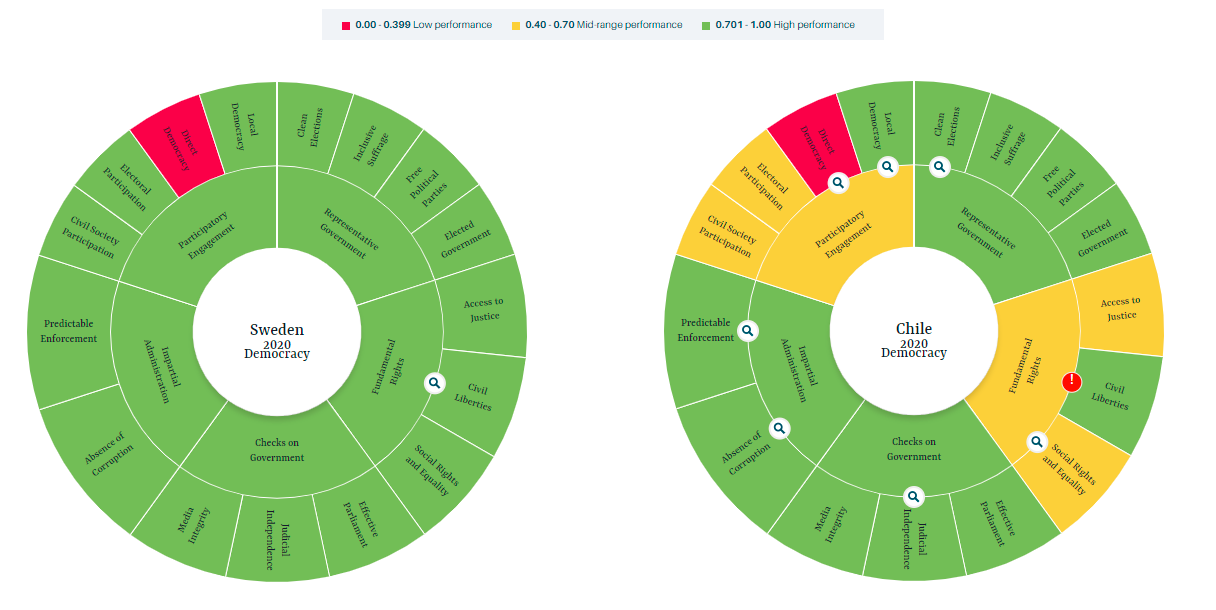
\includegraphics{input/images/Chile-Suecia_DI.PNG}

Respecto a la garantía de derechos fundamentales, Chile ha presentado problemas sobre la Integridad Personal y Seguridad, pues existen casos de uso excesivo de la fuerza por agentes del estado, de hecho, la ``Justicia chilena procesó a nueve militares por delitos de tortura contra un grupo de jóvenes'' . Además, ``Desde octubre de 2019, cuando comenzaron las protestas que dejaron unas 30 personas muertas y miles de heridos y detenidos, se han abierto más de 4.600 casos contra agentes policiales o militares''. En línea con estas faltas al debido proceso, se han registrado casos de detenciones arbitrarias (DI, 2021).

Respecto al compromiso con la participación, Chile, a diferencia de Suecia presenta un desempeño no optimo en dos dimensiones, en la participación electoral y en la participación civil. La participación electoral chilena difícilmente supera el 50\% en las elecciones, lo cual ocurre desde la eliminación del voto obligatorio en el 2013. Por su parte Suecia logra alrededor de un 87\% de participación {[}IDEA{]} (\url{https://www.idea.int/data-tools/country-view/261/40}).
En suma, aunque ambos países tienen gobiernos representativos, la democracia de Suecia destaca en la garantía de derechos sociales y de acceso a la justicia, así como también destaca en el involucramiento político.

\hypertarget{comparaciuxf3n-historica-de-la-calidad-de-la-democracia}{%
\section{Comparación historica de la calidad de la democracia}\label{comparaciuxf3n-historica-de-la-calidad-de-la-democracia}}

En esta sección se describirá el desempeño de la democracia chilena y sueca en distintos ámbitos a lo largo del tiempo. Los gráficos solo incluyen información desde 1975 hasta el 2020. Los gráficos provienen directamente de la plataforma virtual de visualización de datos de el Índice de la Democracia \href{https://www.idea.int/gsod-indices/compare-countries-regions}{(IDEA, 2022)}.

En el primer grafico se puede apreciar el desempeño de Chile y Suecia en una dimensión elemental de la democracia, la elección democrática del gobierno. Como se puede apreciar, aunque ambos países cuentan actualmente con niveles adecuados de la representatividad del gobierno, estos tienen historias y trayectorias distintas.

Las diferentes trayectorias de la democracia en ambos países poseen un efecto en la vida ciudadana. Mientras Suecia ha sido una democracia estable durante los últimos 50 años, Chile es una democracia desde 1990, pues desde 1973 hasta dicha fecha tuvo un gobierno dictatorial. Esto posee como consecuencia que varías cortes crecieron y vivieron su ciudadanía en un contexto donde la política y los partidos estaban prohibidos y eran perseguidos. Esto tiene como implicancia que varías generaciones, que incluso nacieron en democracia, se crían con padres que tuvieron una relación lejana con la democracia. {[}Buscar cita de efecto cohorte autoritarismo{]}.

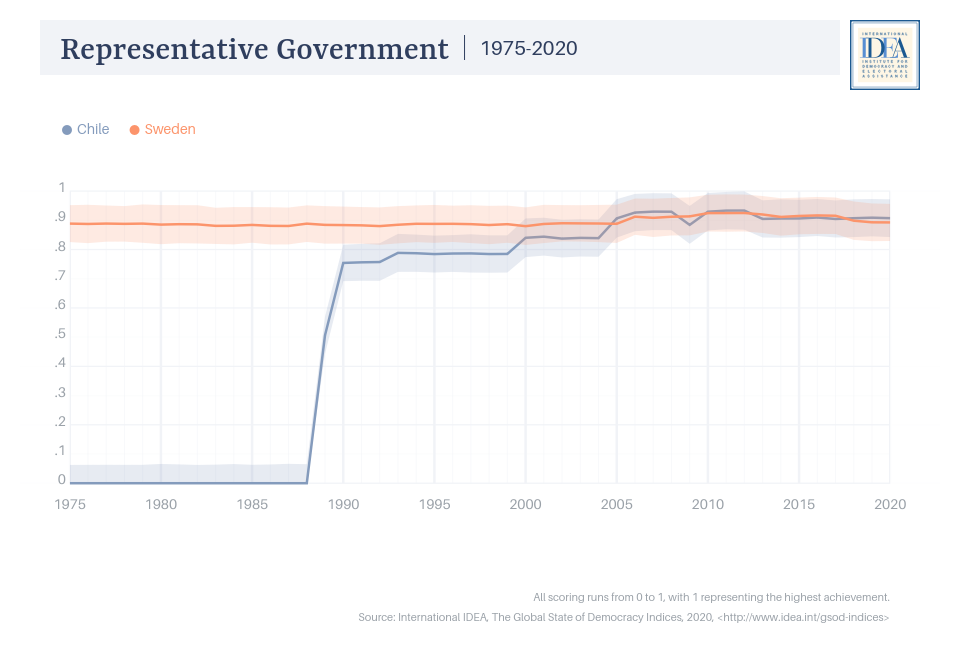
\includegraphics{input/images/representative-government_1975-2020.png}

Los años de ausencia de la democracia se hacen presentes en las prácticas democráticas de los ciudadanos Chilenos. Suecia posee una alta participación, que es tan estable como lo ha sido su democracia. Por su parte, en Chile se puede observar un gran aumento de la participación al finalizar la democracia en 1990, no obstante, mientras avanza el periodo democrático se observa un descenso en esa participación. Respecto a la participación de los ciudadanos en organizaciones de la sociedad civil se destaca que Suecia posee una mayor participación que Chile, aunque este el de este ultimo ha crecido ligeramente en estos años, además del gran repunte posterior al fin de la dictadura Chilena. Por su parte, Suecia desciende ligeramente en este ámbito.

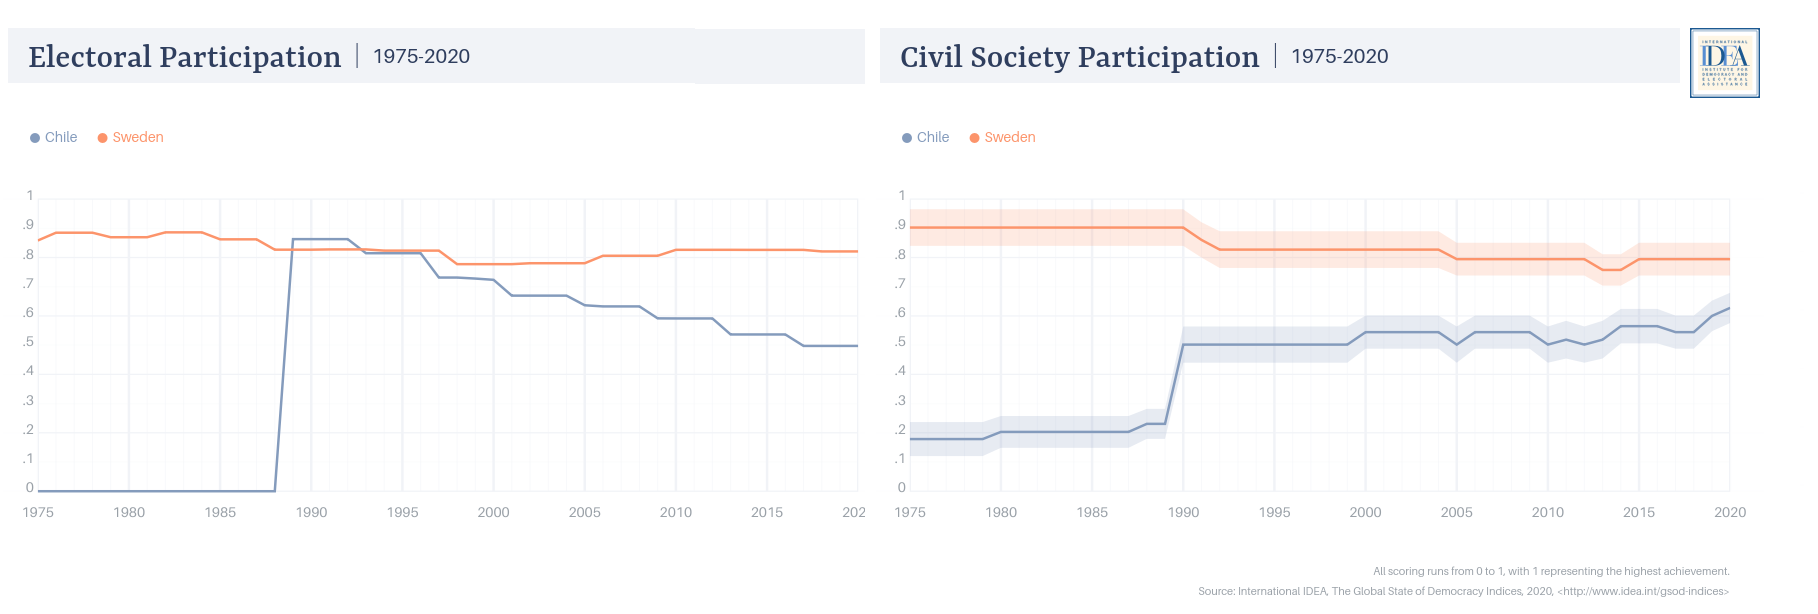
\includegraphics{input/images/electoral-participation_1975-2020.png}

Junto con esta falta de participación de Chile, se puede observar un mejor cumplimiento de objetivos democráticos como la garantía de los derechos fundamentales y la administración imparcial por parte de Suecia respecto a Chile. En ambos ámbitos se puede observar que Suecia ha tenido un alto y estable desempeño, mientras que Chile tuvo en el periodo dictatorial un bajo desempeño. Algunos autores han señalado que la falta de garantía en los derechos de distintos países fomenta distintas visiones de lo que es un buen ciudadano, de modo tal que en aquellas democracias con mejor garantía de derechos fomentan visiones de ciudadanos más centradas en el la norma democrática que en la crítica. En una línea similar, y en relación con la imparcialidad de la administración, se ha señalado que las sensaciones de injusticias (que pueden ser producidas por tratos diferenciados) pueden fomentar actitudes de insubordinación.

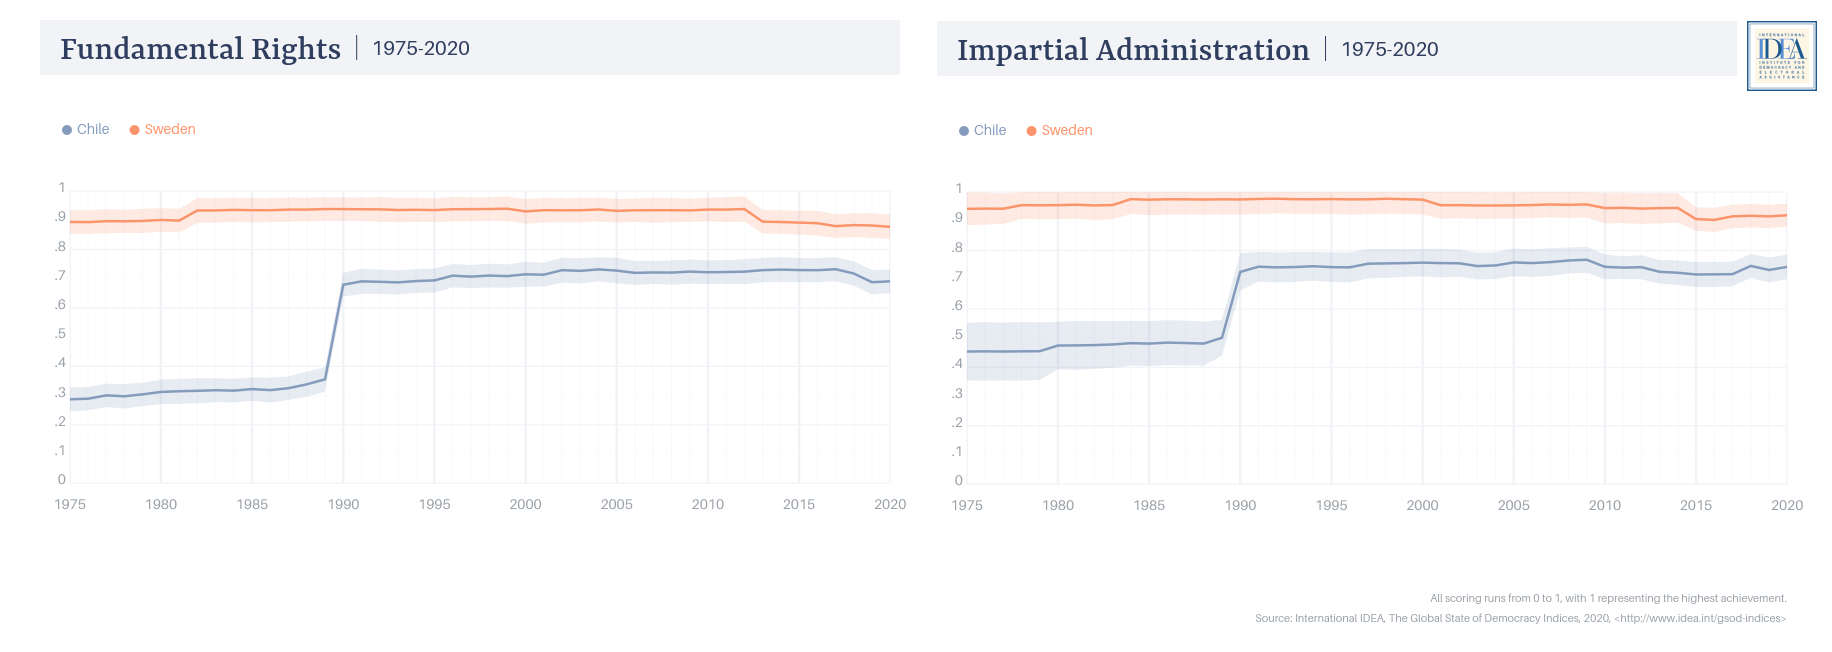
\includegraphics{input/images/fundamental-rights_1975-2020.png}

x

\hypertarget{la-democracia-seguxfan-los-ciudadnos-comparaciuxf3n-de-la-opinion-publica-de-chile-y-suecia}{%
\chapter{La democracia según los ciudadnos: comparación de la opinion publica de Chile y Suecia}\label{la-democracia-seguxfan-los-ciudadnos-comparaciuxf3n-de-la-opinion-publica-de-chile-y-suecia}}

Esta apartado explora la opinión publica de los adultos de ambos países sobre 3 temas relativos a las vivencias democráticas. En particular compararemos la evaluación de los ciudadanos sobre sus democracias, intentaremos contrastar sus valores democráticos y su relación con la participación democrática.

Para realizar estas comparaciones se utiliza la encuesta internacional de valores, utilizando la información longitudinal disponible para Chile y Suecia entre 1989 y 2019. Para este analisis se cuenta con 9918 casos de ciudadanos de ambos países para las distintas olas de este estudio. En el caso de Chile se cuenta con el periodo completo, mientras que para los datos suecos solo se cuenta con las olas desde 1994 y el 2014

\hypertarget{opinion-sobre-su-democracia}{%
\section{Opinion sobre su democracia}\label{opinion-sobre-su-democracia}}

\begin{quote}
Satisfacción con el desempeño de la democraica E110
\end{quote}

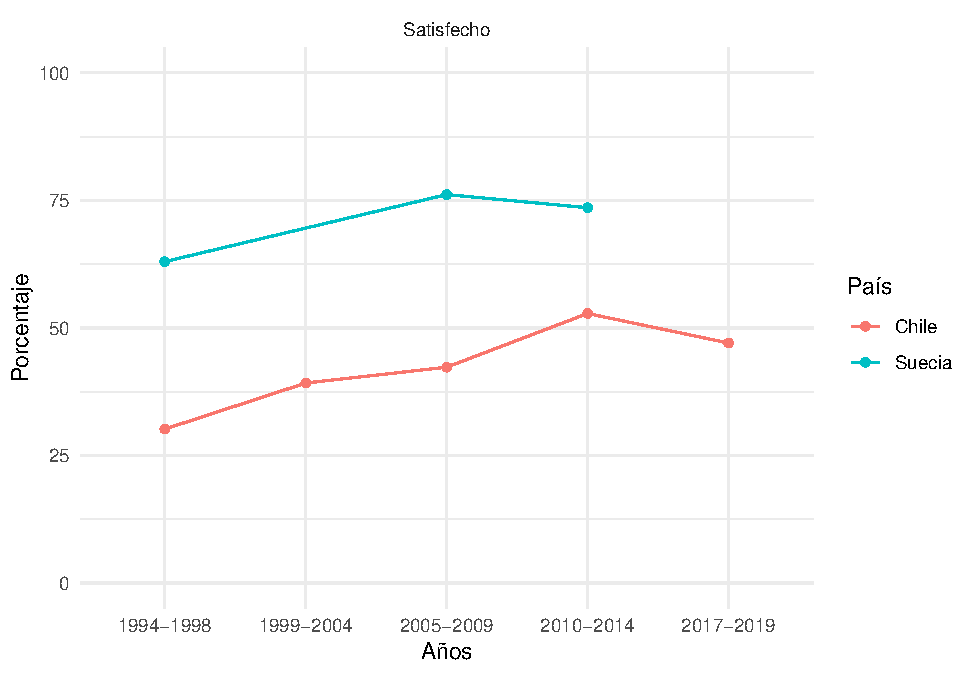
\includegraphics[width=0.8\linewidth,]{Chile_Suecia_files/figure-latex/unnamed-chunk-6-1}

\begin{quote}
Confianza en el gobierno E069\_11
\end{quote}

\begin{quote}
Confianza en el parlamento E069\_07
\end{quote}

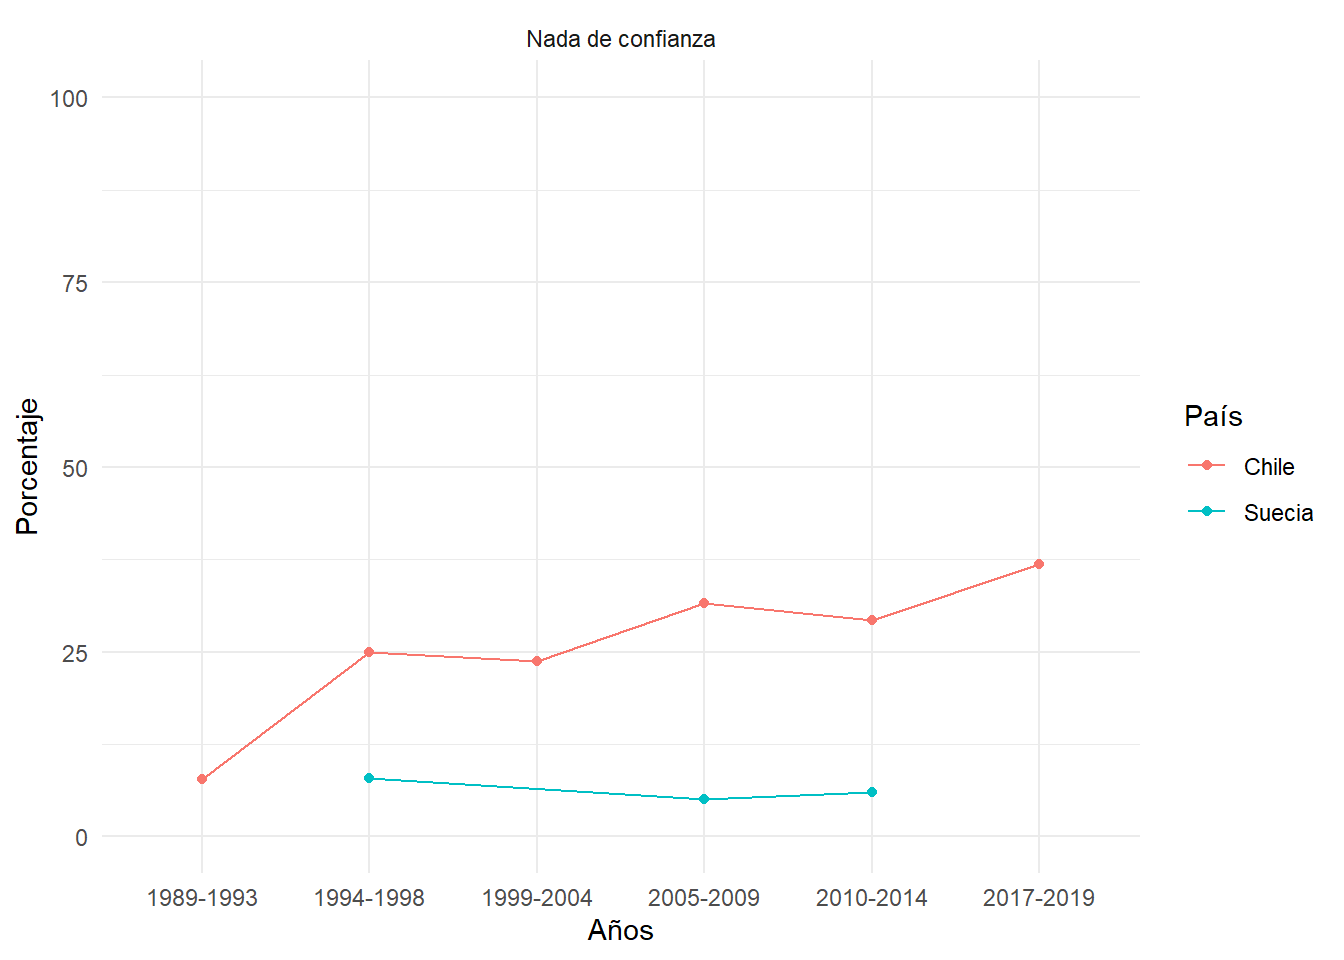
\includegraphics[width=0.8\linewidth,]{Chile_Suecia_files/figure-latex/unnamed-chunk-7-1}

\hypertarget{valores-democraticos}{%
\section{Valores democraticos}\label{valores-democraticos}}

\begin{quote}
prioridad nacionales C002
\end{quote}

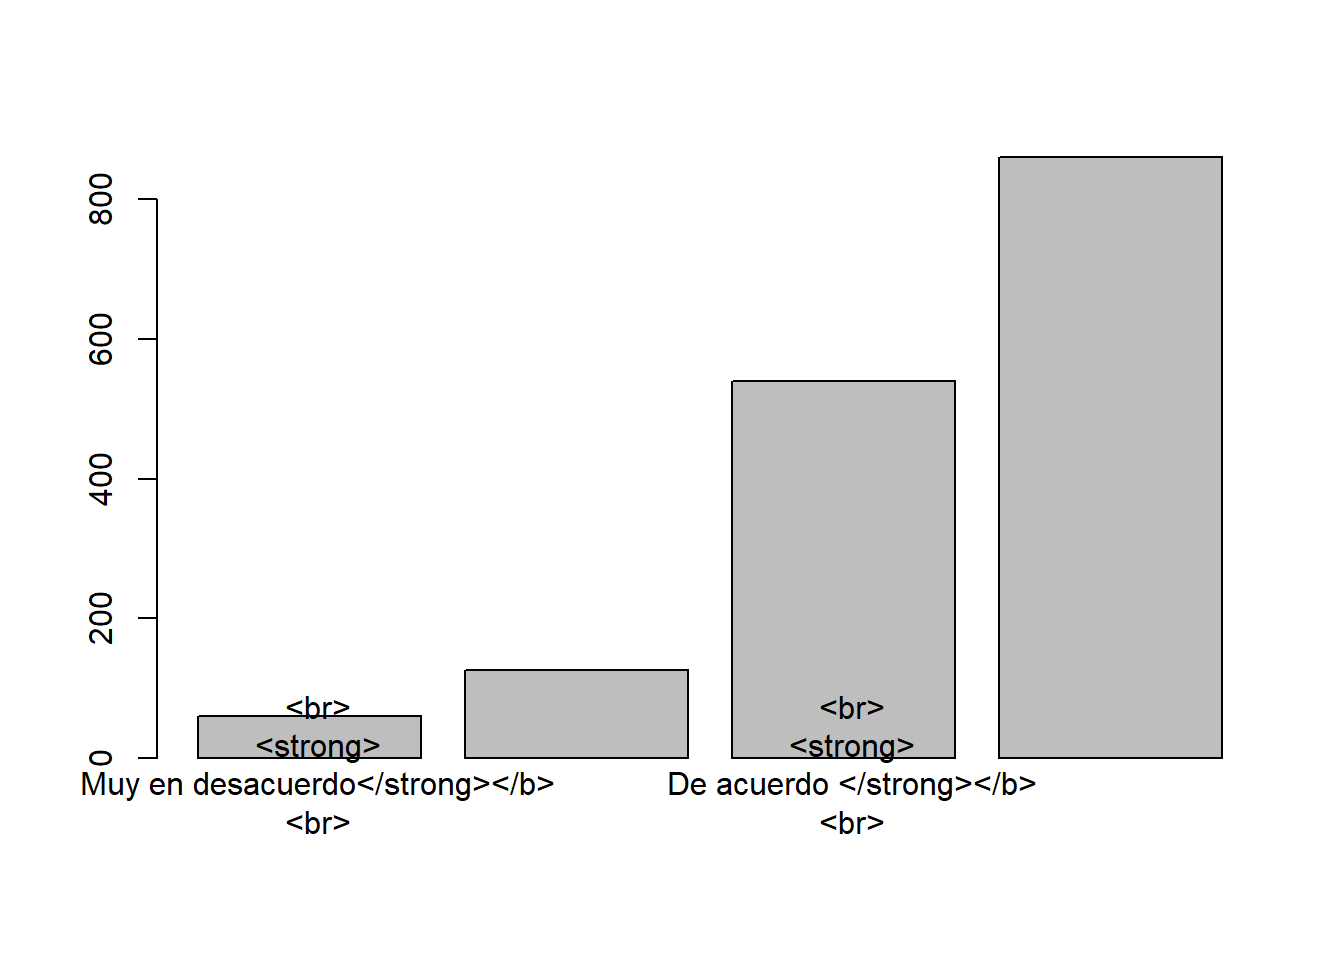
\includegraphics[width=0.8\linewidth,]{Chile_Suecia_files/figure-latex/unnamed-chunk-8-1}

\hypertarget{participaciuxf3n-en-adultos}{%
\section{Participación en Adultos}\label{participaciuxf3n-en-adultos}}

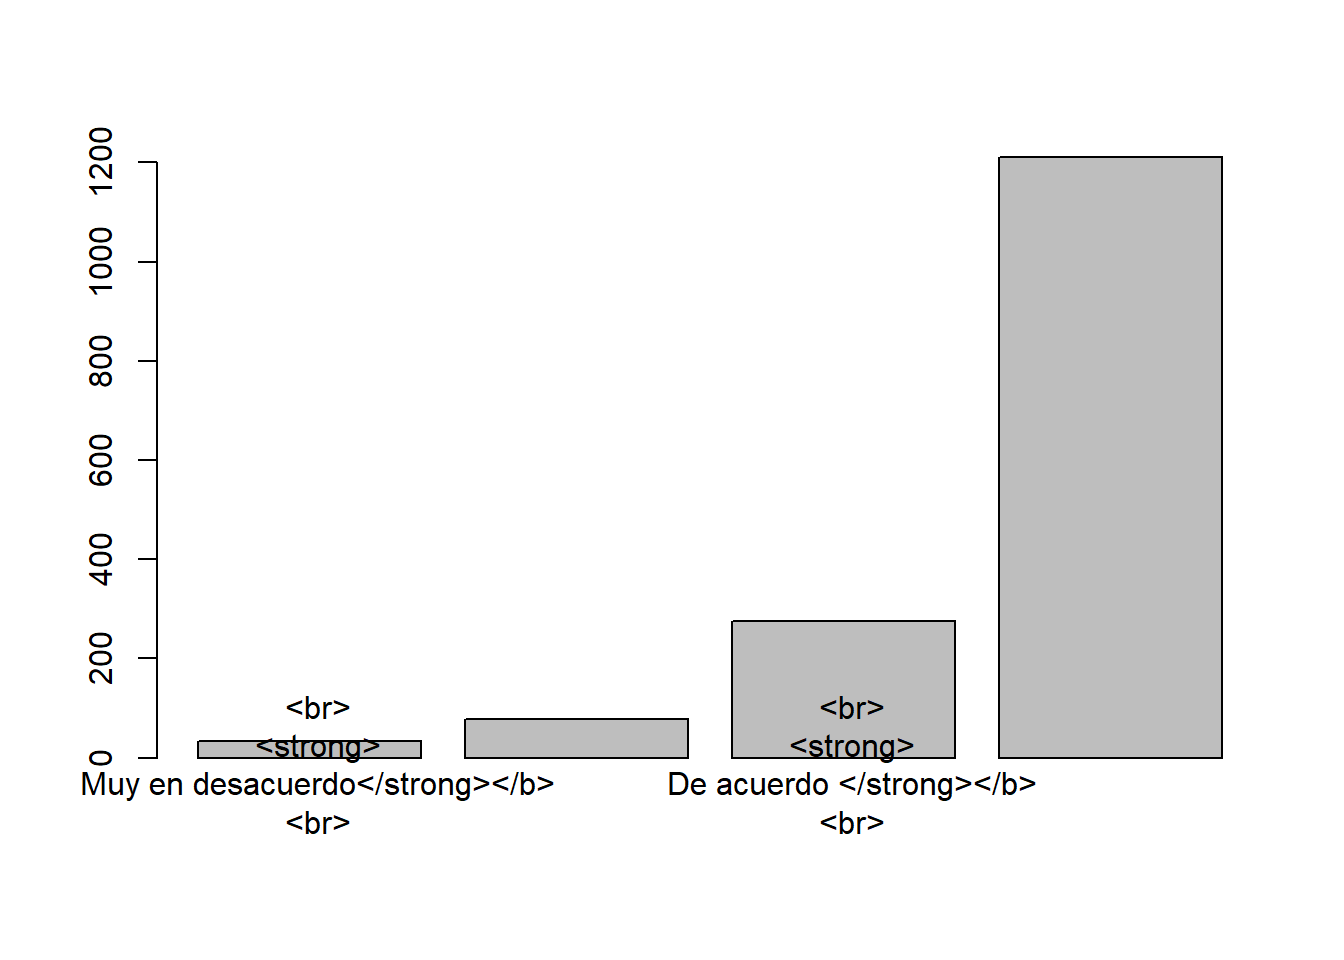
\includegraphics[width=0.8\linewidth,]{Chile_Suecia_files/figure-latex/unnamed-chunk-9-1}
320 E027 Acción política: asistencia a manifestaciones lícitas/pacíficas
397 E110 Satisfacción con el desarrollo de la democracia
405 E117 Sistema político: Tener un sistema político democrático
408 E120 En democracia, el sistema económico funciona mal
436 E221B Acción política realizada recientemente: Asistir a manifestaciones pacíficas/lícitas
449 E235 Importancia de la democracia

Sobre pariticpación politica chile tien euna alta manifestacion en el periodo final de la dictadura, luego se calma con la democracia y luego vuelve a crecer desde el 2010 hasta llegar al 2019

La pregunta de satisfacción democracia no esta en la base de datos

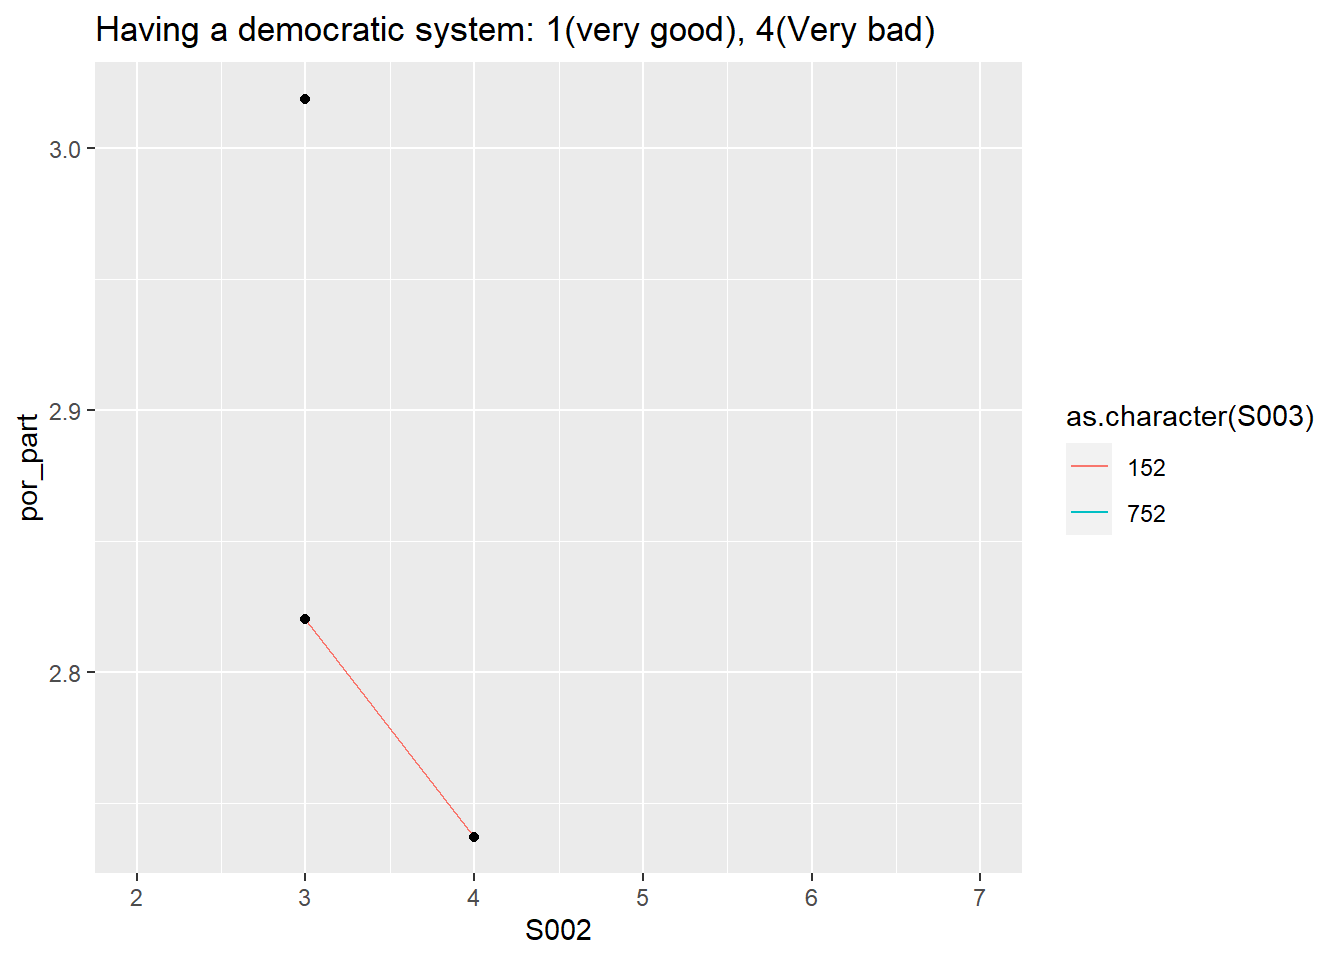
\includegraphics[width=0.8\linewidth,]{Chile_Suecia_files/figure-latex/unnamed-chunk-10-1}

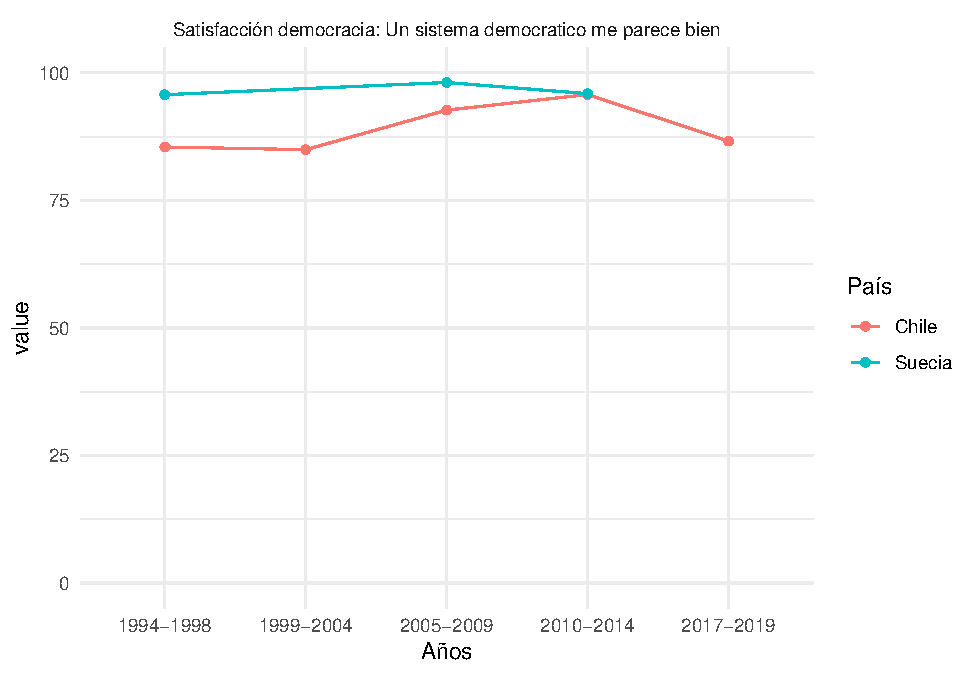
\includegraphics[width=0.8\linewidth,]{Chile_Suecia_files/figure-latex/unnamed-chunk-11-1}

\hypertarget{comparaciuxf3n-de-la-vivencia-democratica-juvenil}{%
\chapter{Comparación de la vivencia democratica juvenil}\label{comparaciuxf3n-de-la-vivencia-democratica-juvenil}}

El presente apartado compara las experiencias con la ciudadanía de los jóvenes de Chile y Suecia. Para ello, se contrastan las opiniones, valores y practicas relativas a la democracia de ambos países en población estudiantil con las mismas edades. Sobre la opinión respecto a su democracia, se describirá el nivel de satisfacción con la democracia de los jóvenes de ambos países, así como sobre su confianza en las instituciones democráticas. Para comparar los valores democráticos, se revisará sus concepciones de un buen ciudadano y sus opiniones sobre la igualdad de derechos. Finalmente se contrasta la participación democrática en la esfera pública, en la escuela y con sus cercanos.

Para enriquecer la comparación, se hará referencia constante a los elementos del contexto de cada país revisados anteriormente. El contraste de la experiencia democrática juvenil de ambos países se hará destacando la calidad de la democracia de ambos países. Al reflexionar sobre las diferencias y similitudes de la experiencia de los jóvenes se tomara en cuenta la calidad de las instituciones democráticas y tanto la participación como la opinión sobre la democracia en la población adulta de ambos países.

\hypertarget{opinion-sobre-su-democracia-1}{%
\section{Opinion sobre su democracia}\label{opinion-sobre-su-democracia-1}}

El siguiente grafico expone la satisfacción con la democracia de los jóvenes de ambos países. En ambos casos se le pregunta respecto a su satisfacción con la democracia de su propio país. La cantidad de categorías de respuesta era la misma en ambas encuestas y los mensajes son bastante similares, aunque solo las categorías extremas son equivalentes.

La satisfacción con la democracia de los jóvenes de ambos países difiere radicalmente, de modo tal que es mucho mayor en Suecia que en Chile. La cantidad de estudiantes nada satisfechos es de 28,2\% en Chile y de 2,7\% en Suecia. Proporcionalmente hablando, por cada estudiante insatisfecho con la democracia en Suecia hay 10 estudiantes insatisfechos con su democracia en Chile.

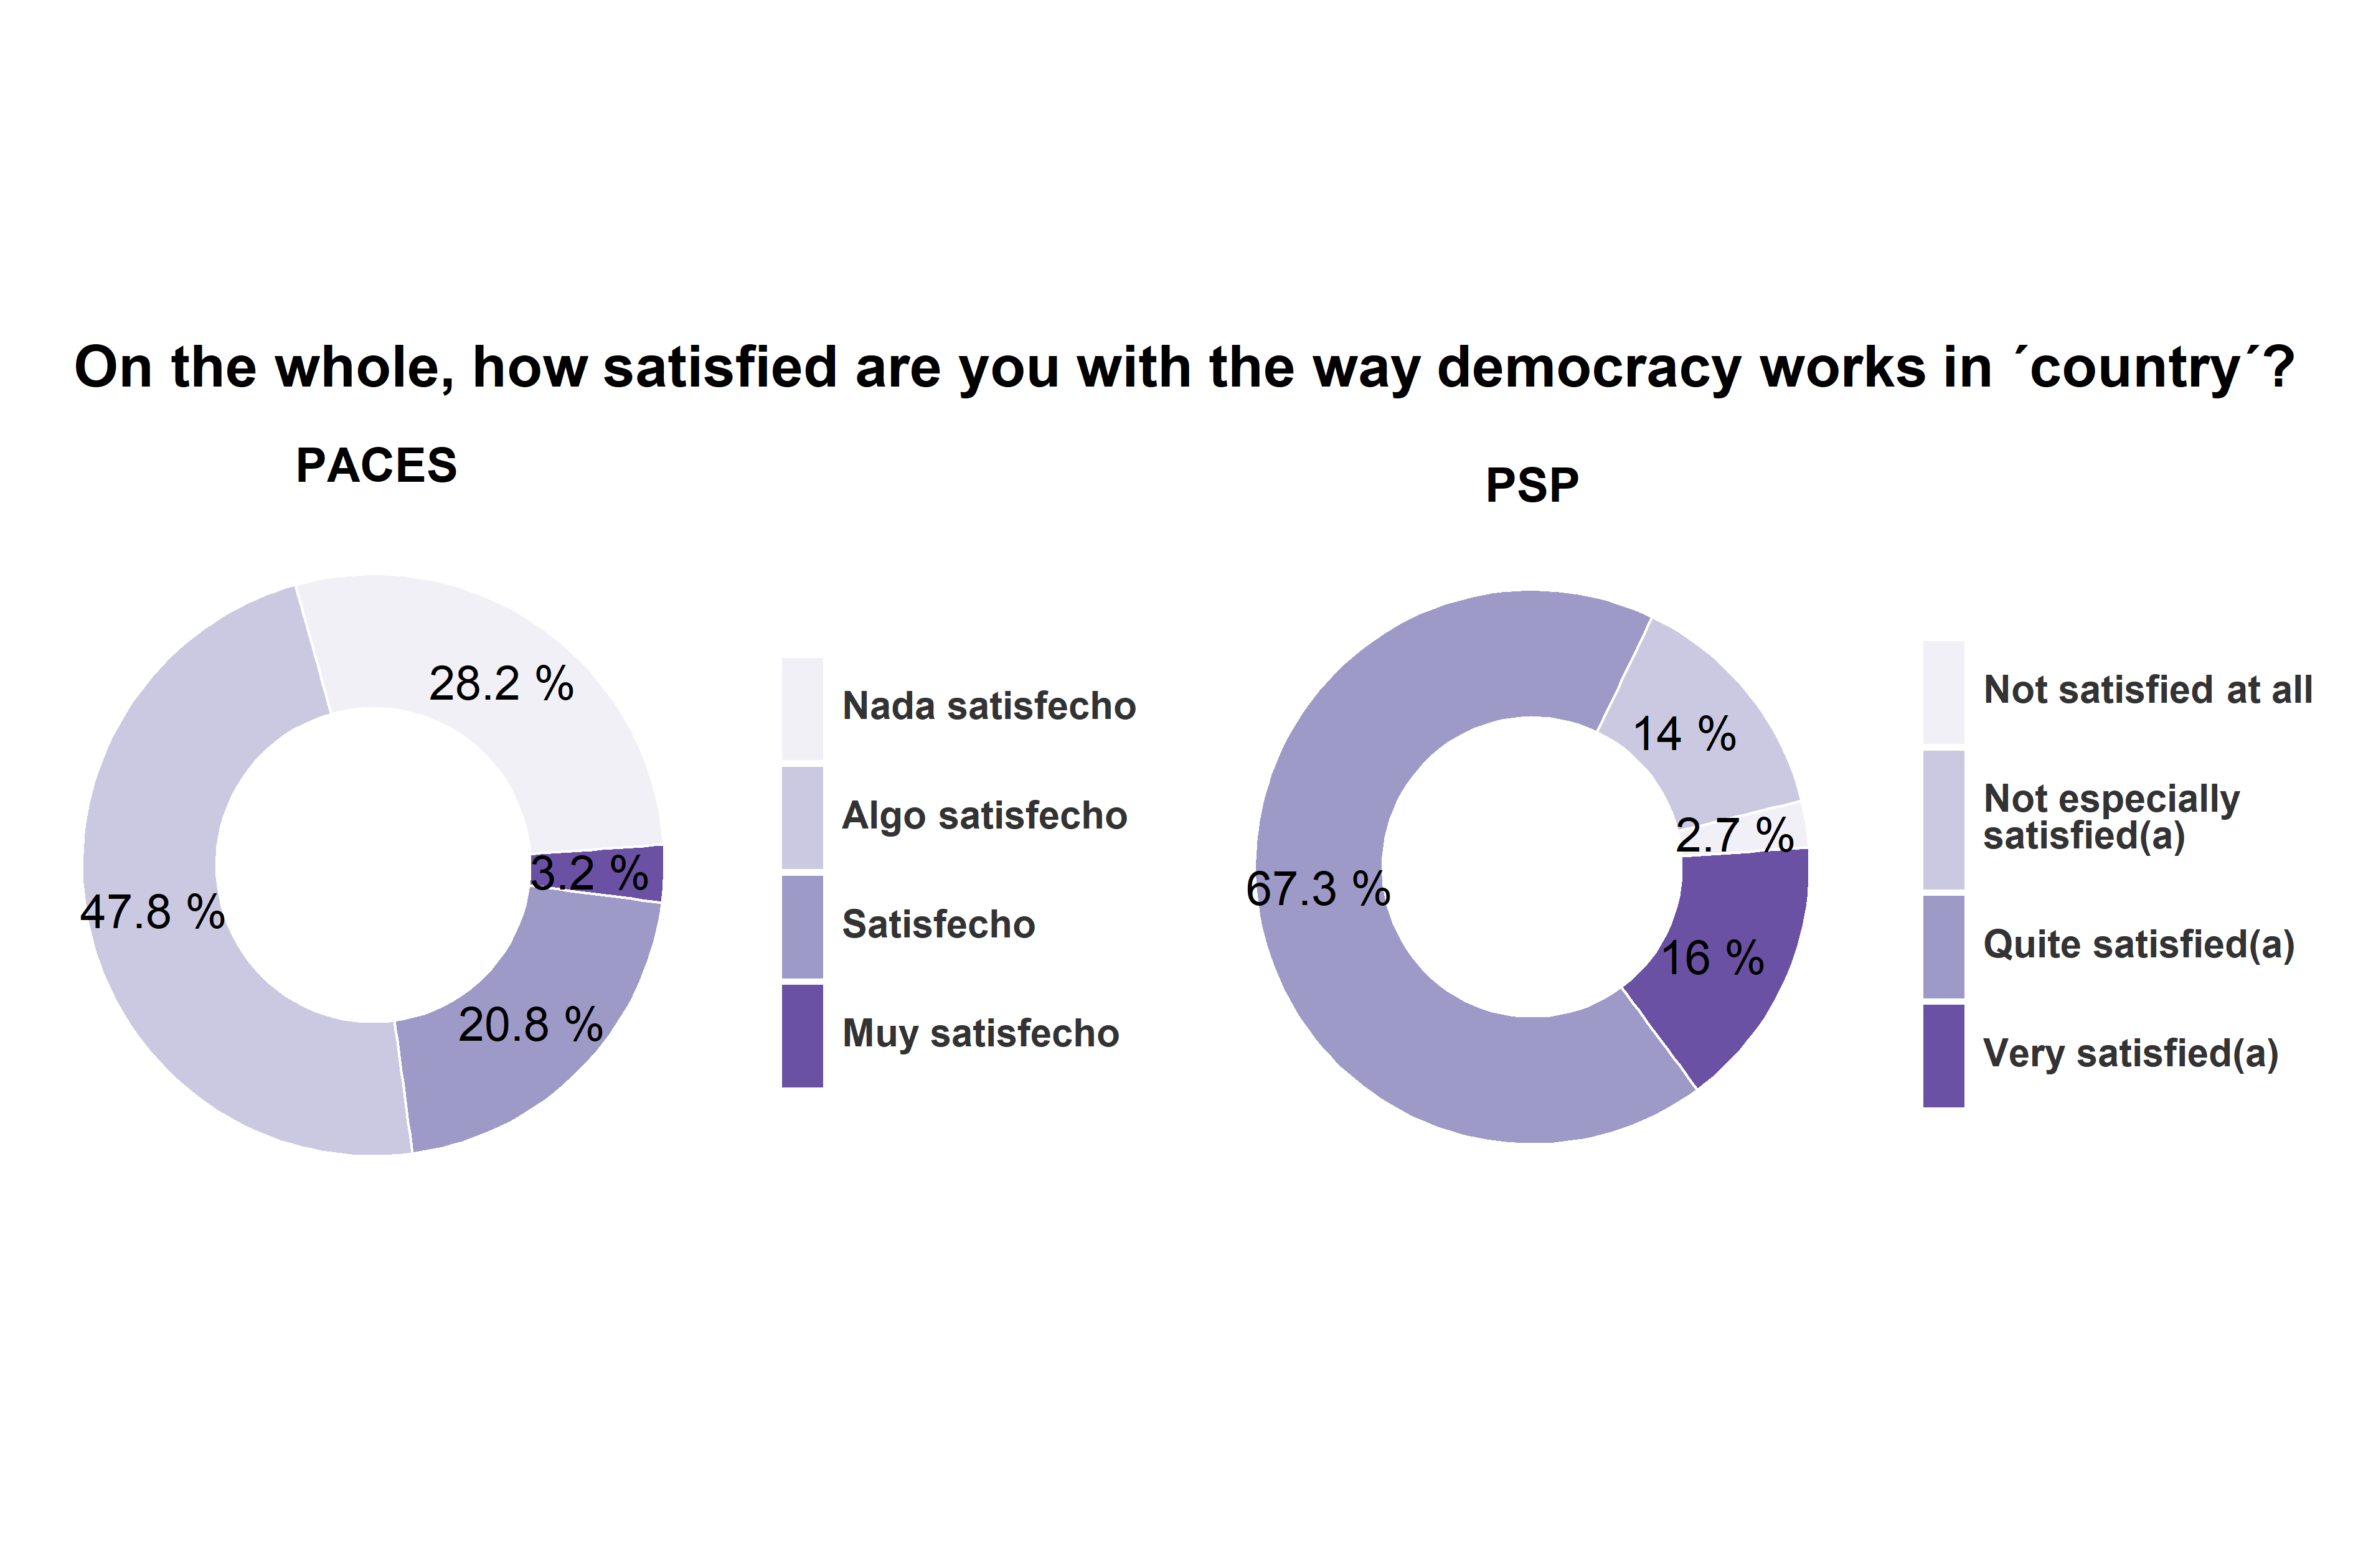
\includegraphics{output/graph_sat.png}

El que los jóvenes suecos estén más satisfechos con su democracia que los jóvenes chilenos es relativamente consistente con la calidad actual de las democracias en ambos países. Aunque según el índice de la democracia actualmente tanto en Chile como en Suecia existe una administración imparcial, controles gubernamentales y un gobierno representativo, existen diferencias sustanciales en otros aspectos. Contrario al caso Sueco, en Chile no existe una garantía real de los derechos fundamentales, ni tampoco existe un adecuado compromiso con la participación. En el caso Chileno es especialmente deficitario el acceso a la justicia y a los derechos sociales. Es razonable considerar que la ausencia de condiciones adecuadas para el desarrollo de una adecuada vida ciudadana merma la satisfacción con la democracia en el caso chileno, lo cual es consistente con la evidencia que destaca la falta de valoración de la democracia ante la falta de derechos sociales adecuados ().

\hypertarget{confianza-en-sus-instituciones-democraticas}{%
\subsubsection{Confianza en sus instituciones democraticas}\label{confianza-en-sus-instituciones-democraticas}}

El grafico venidero compara la confianza que poseen los estudiantes de los partidos políticos de sus países. Ambas preguntas tienen cuatro categorías, pero las alternativas no son equivalentes.

En ambos países existen distintos niveles de confianza en los partidos, destacando la mayor confianza que tienen los jóvenes suecos. En Suecia, más de la mitad de los jóvenes confía bastante o mucho en los partidos, mientras que en Chile esto ocurre solo con el 15\% de los jóvenes. Consecuentemente existe una gran cantidad de jóvenes chilenos con nada de confianza en los partidos, proporcionalmente hablando, por cada estudiante sueco que no confía en los partidos, en chile hay 6 jóvenes que no lo hacen.

Esto es un problema para chile ya que difícilmente se puede confiar en la democracia y las instituciones democrática, si no se confía en sus principales actores, los partidos.
{[}Consecuencia de la baja confianza en partidos{]}

\textbf{Political parties}

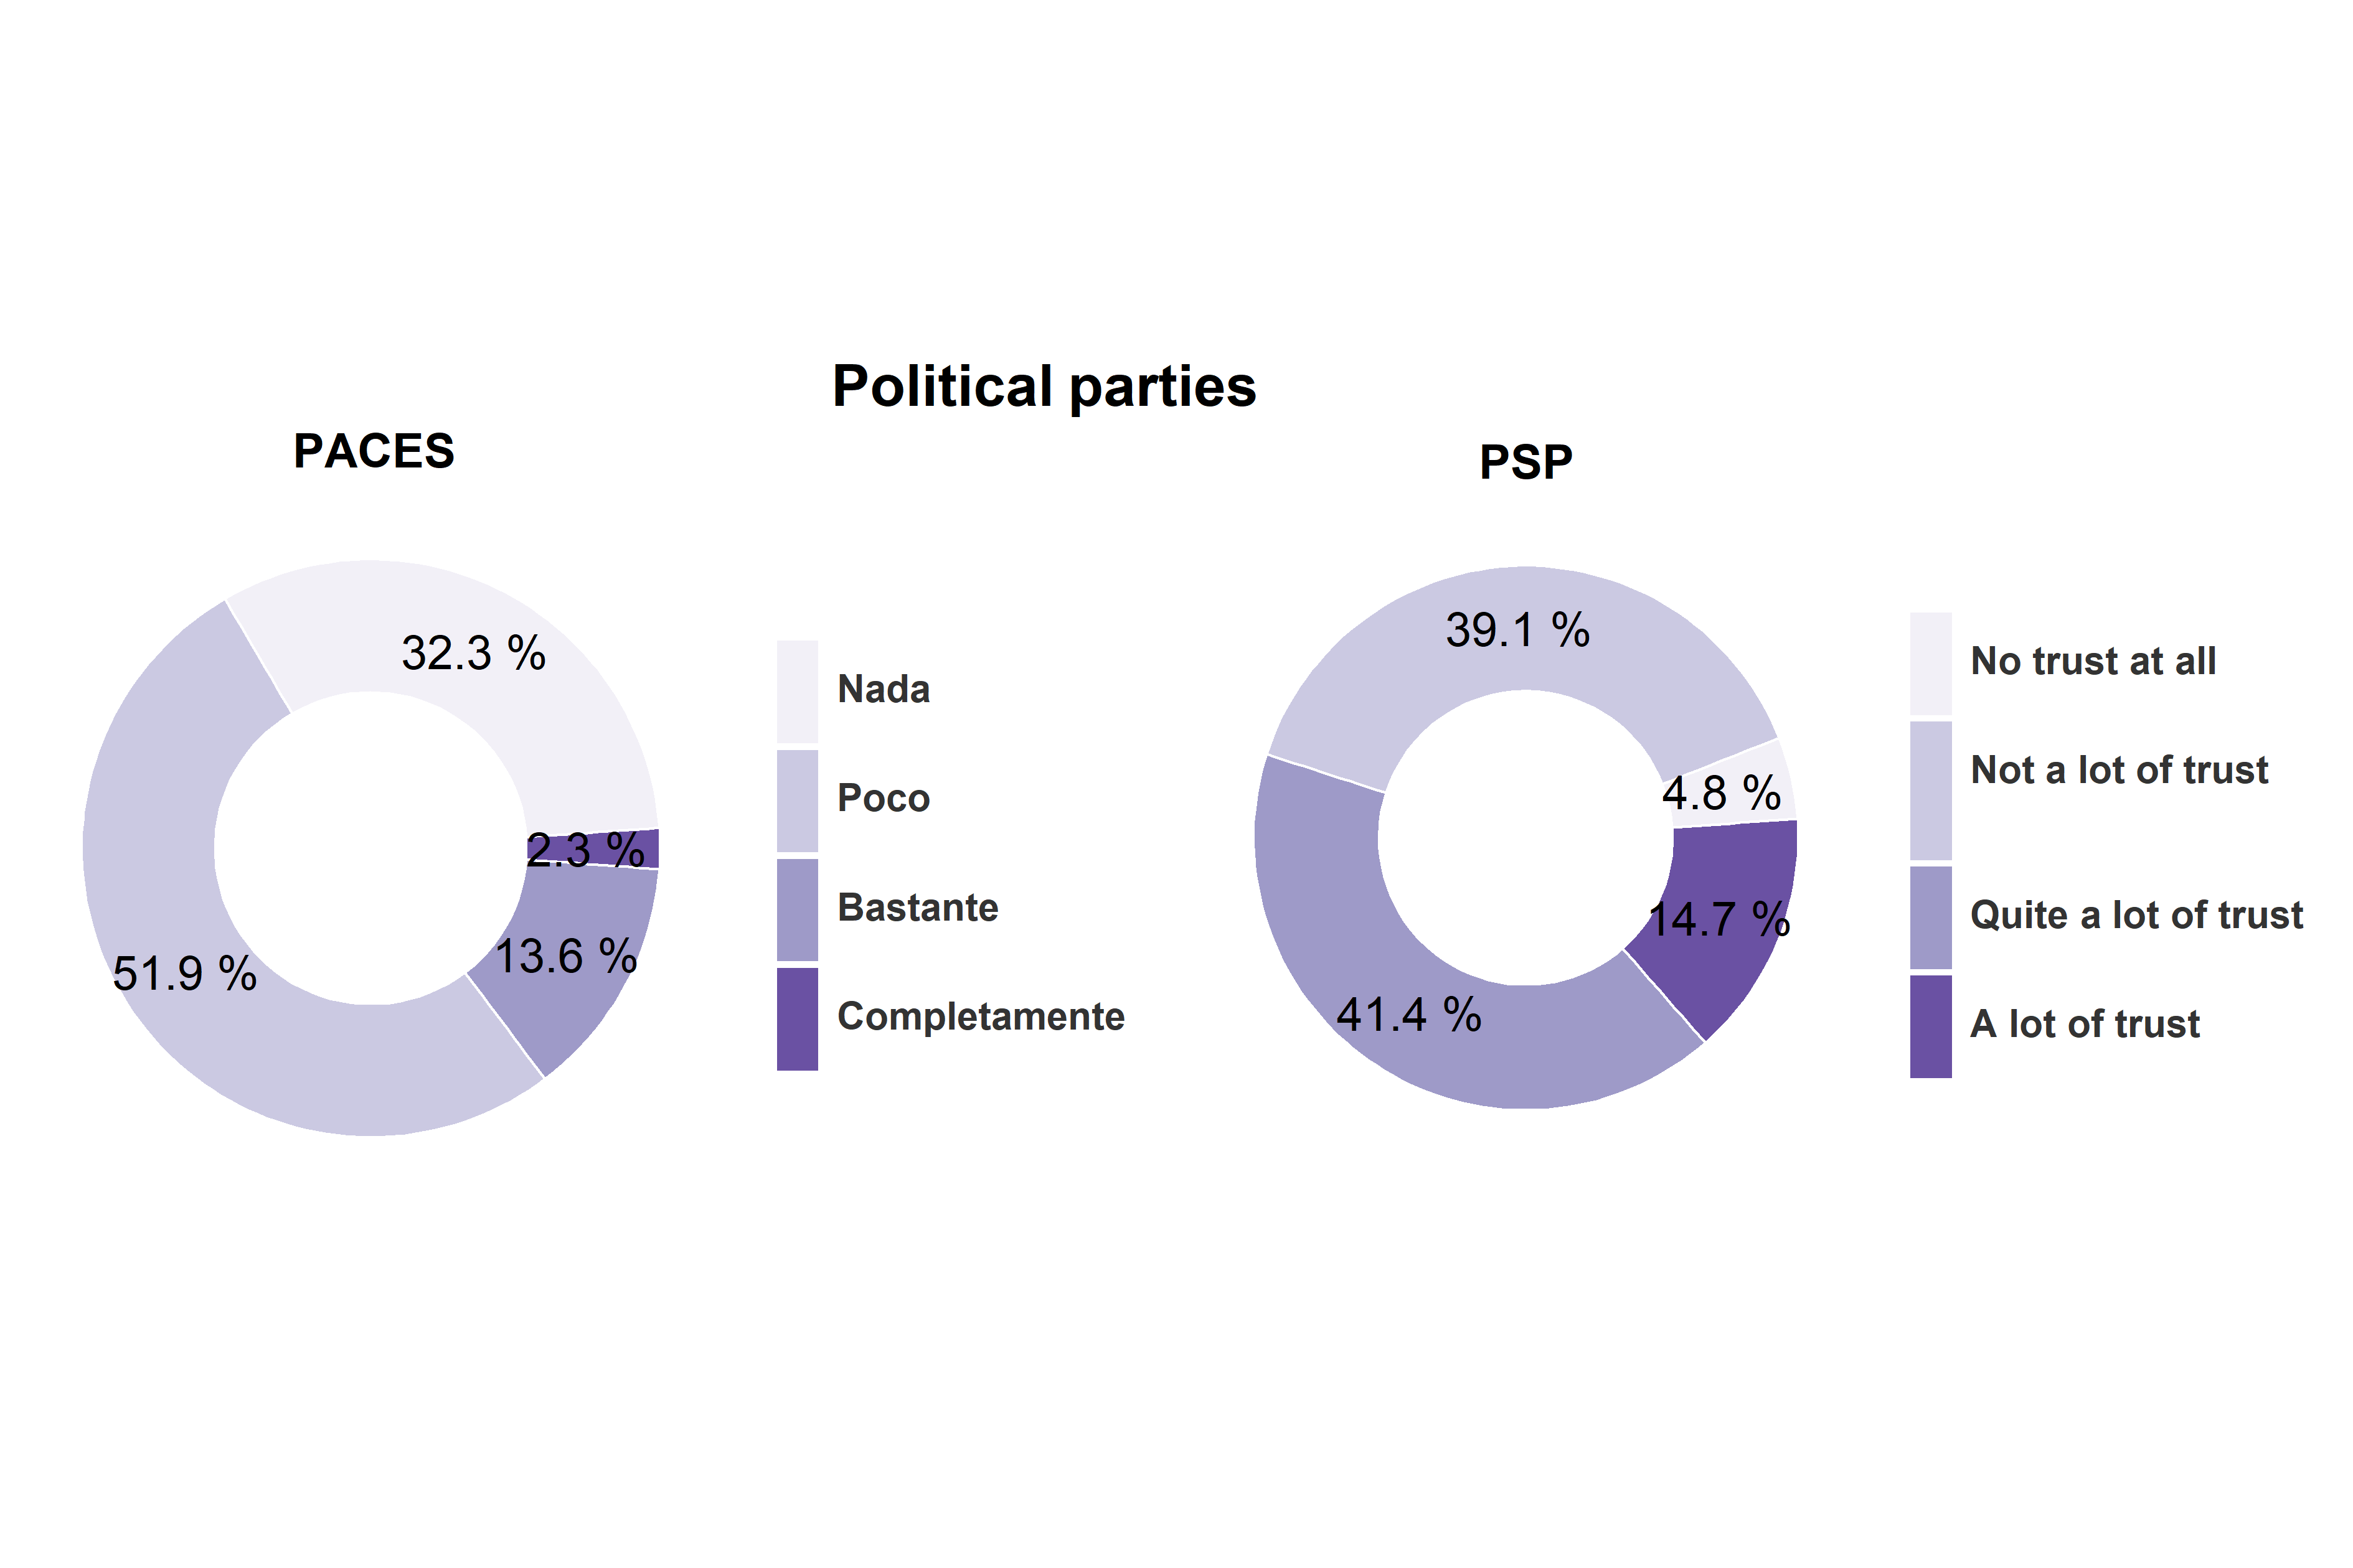
\includegraphics{output/plotru4.png}

\textbf{\#\#\# Trust in people}

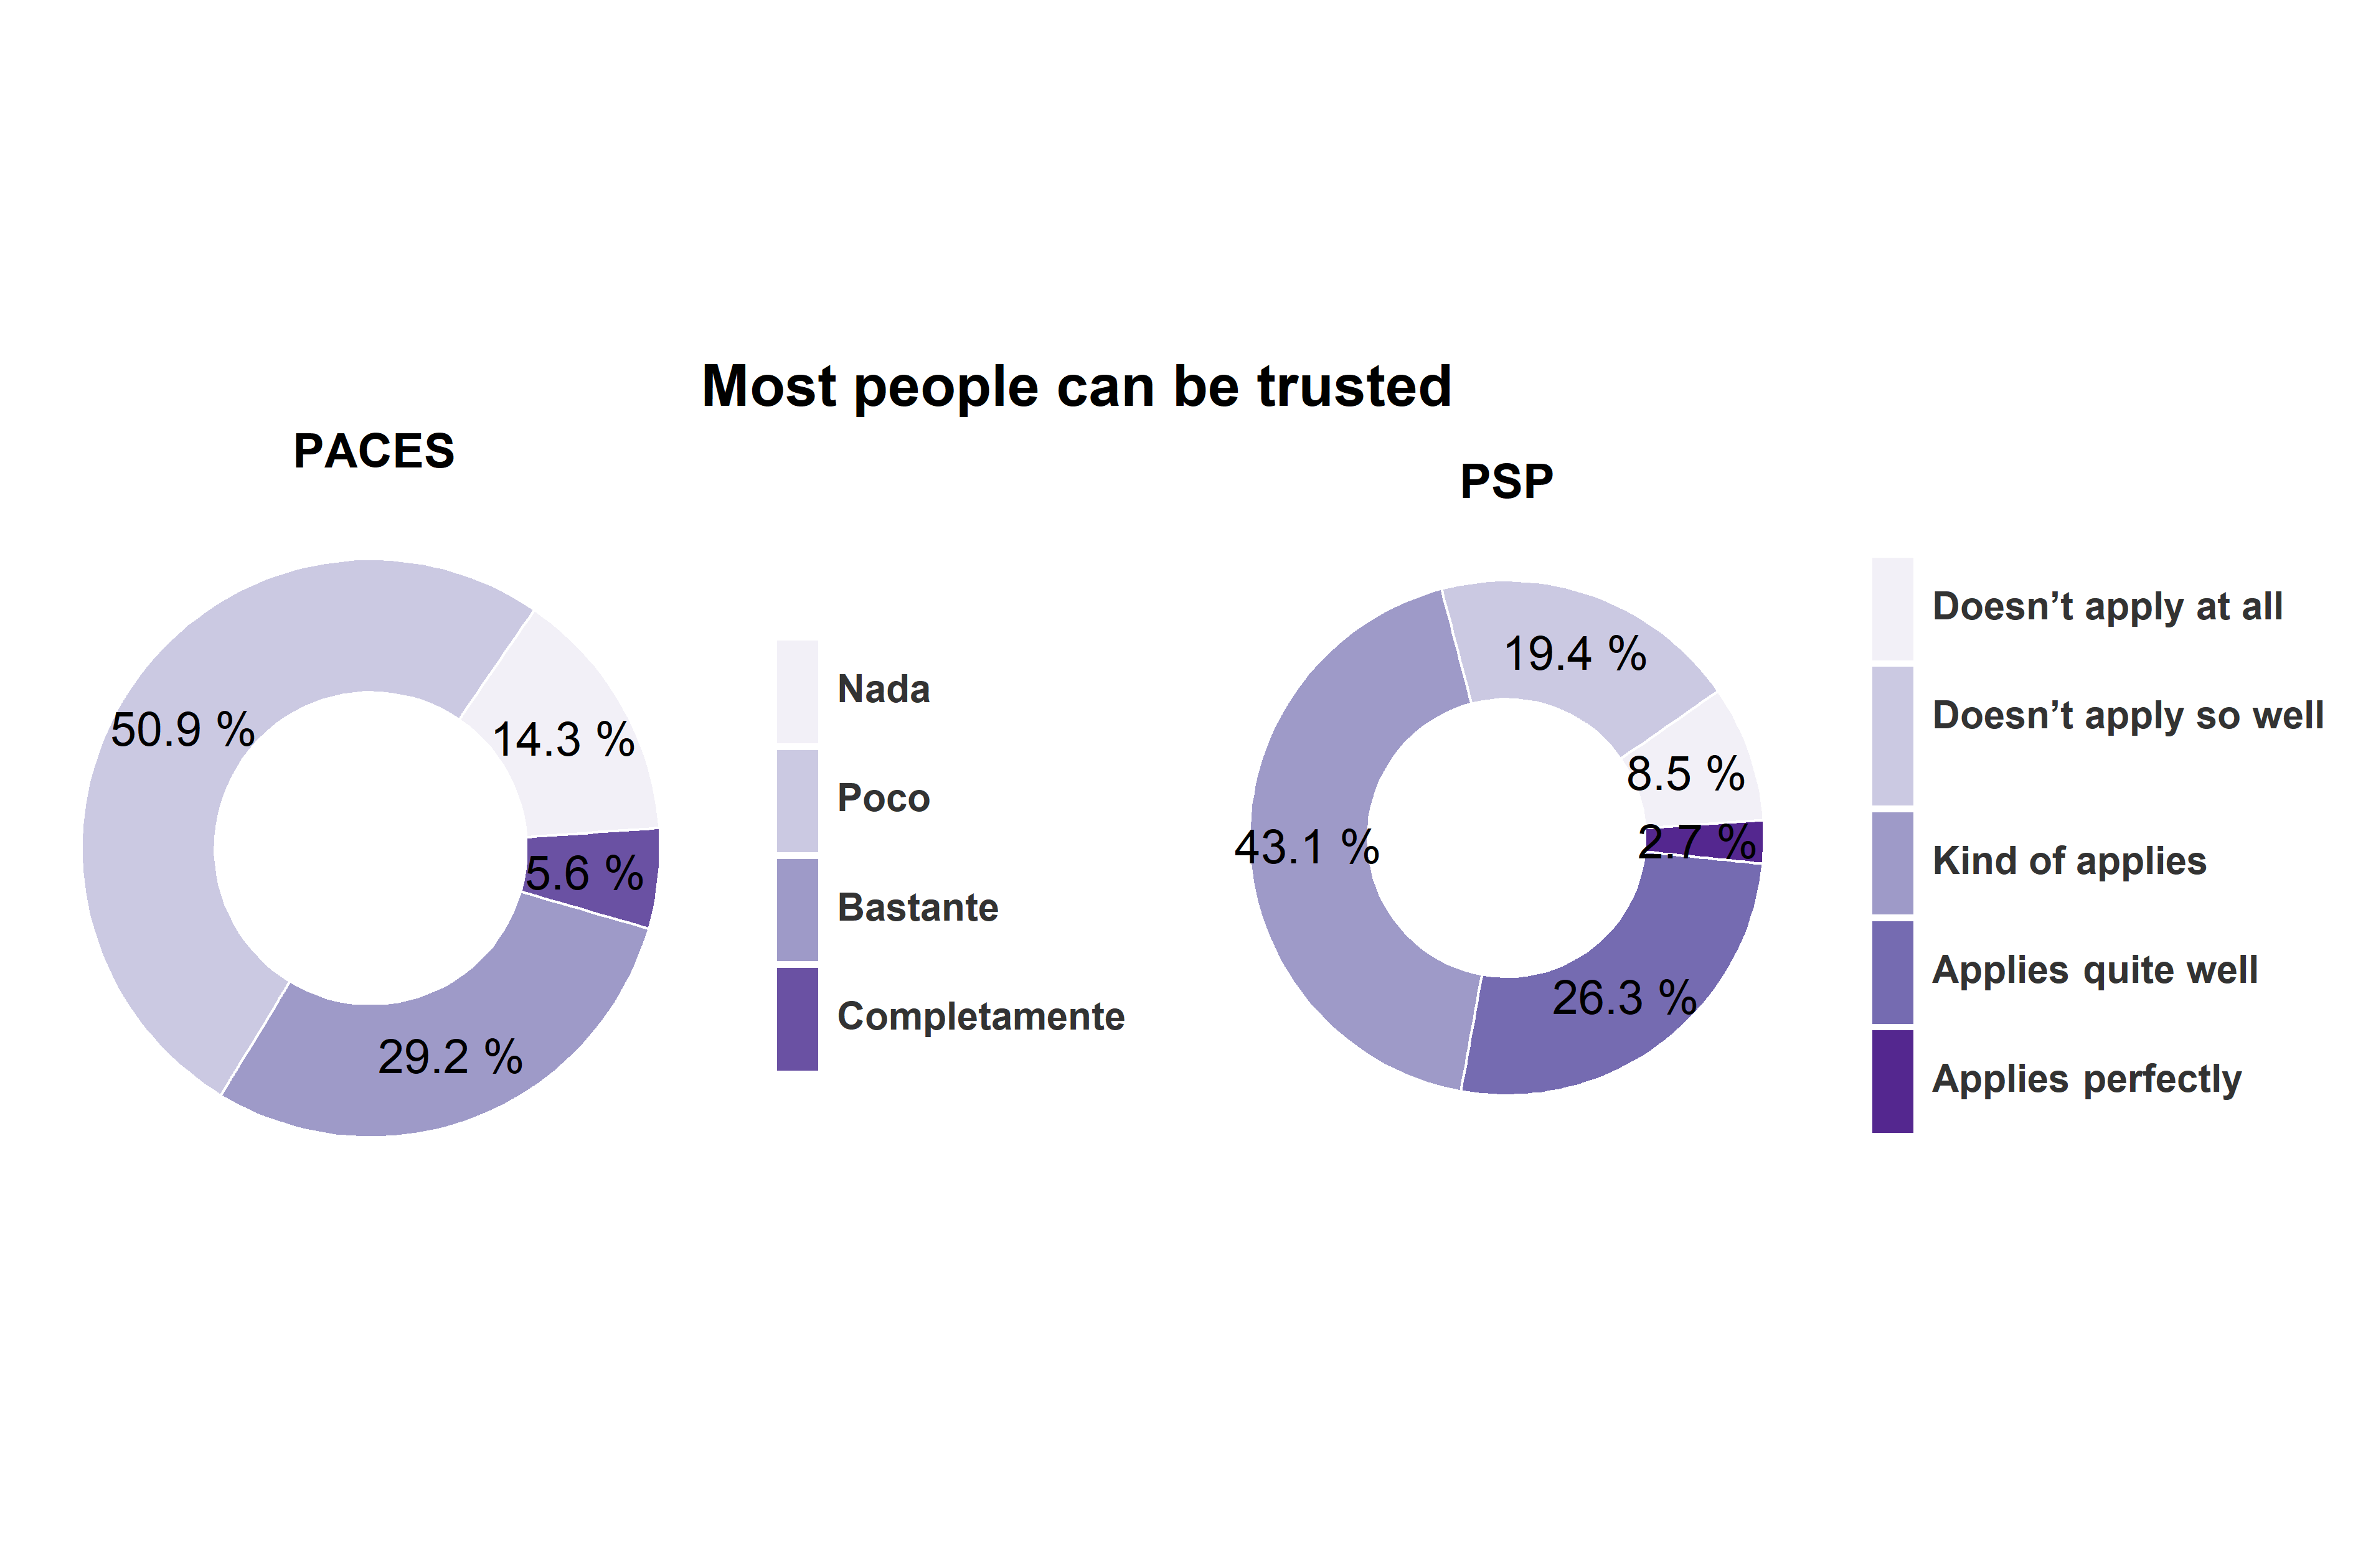
\includegraphics{output/plotru5.png}

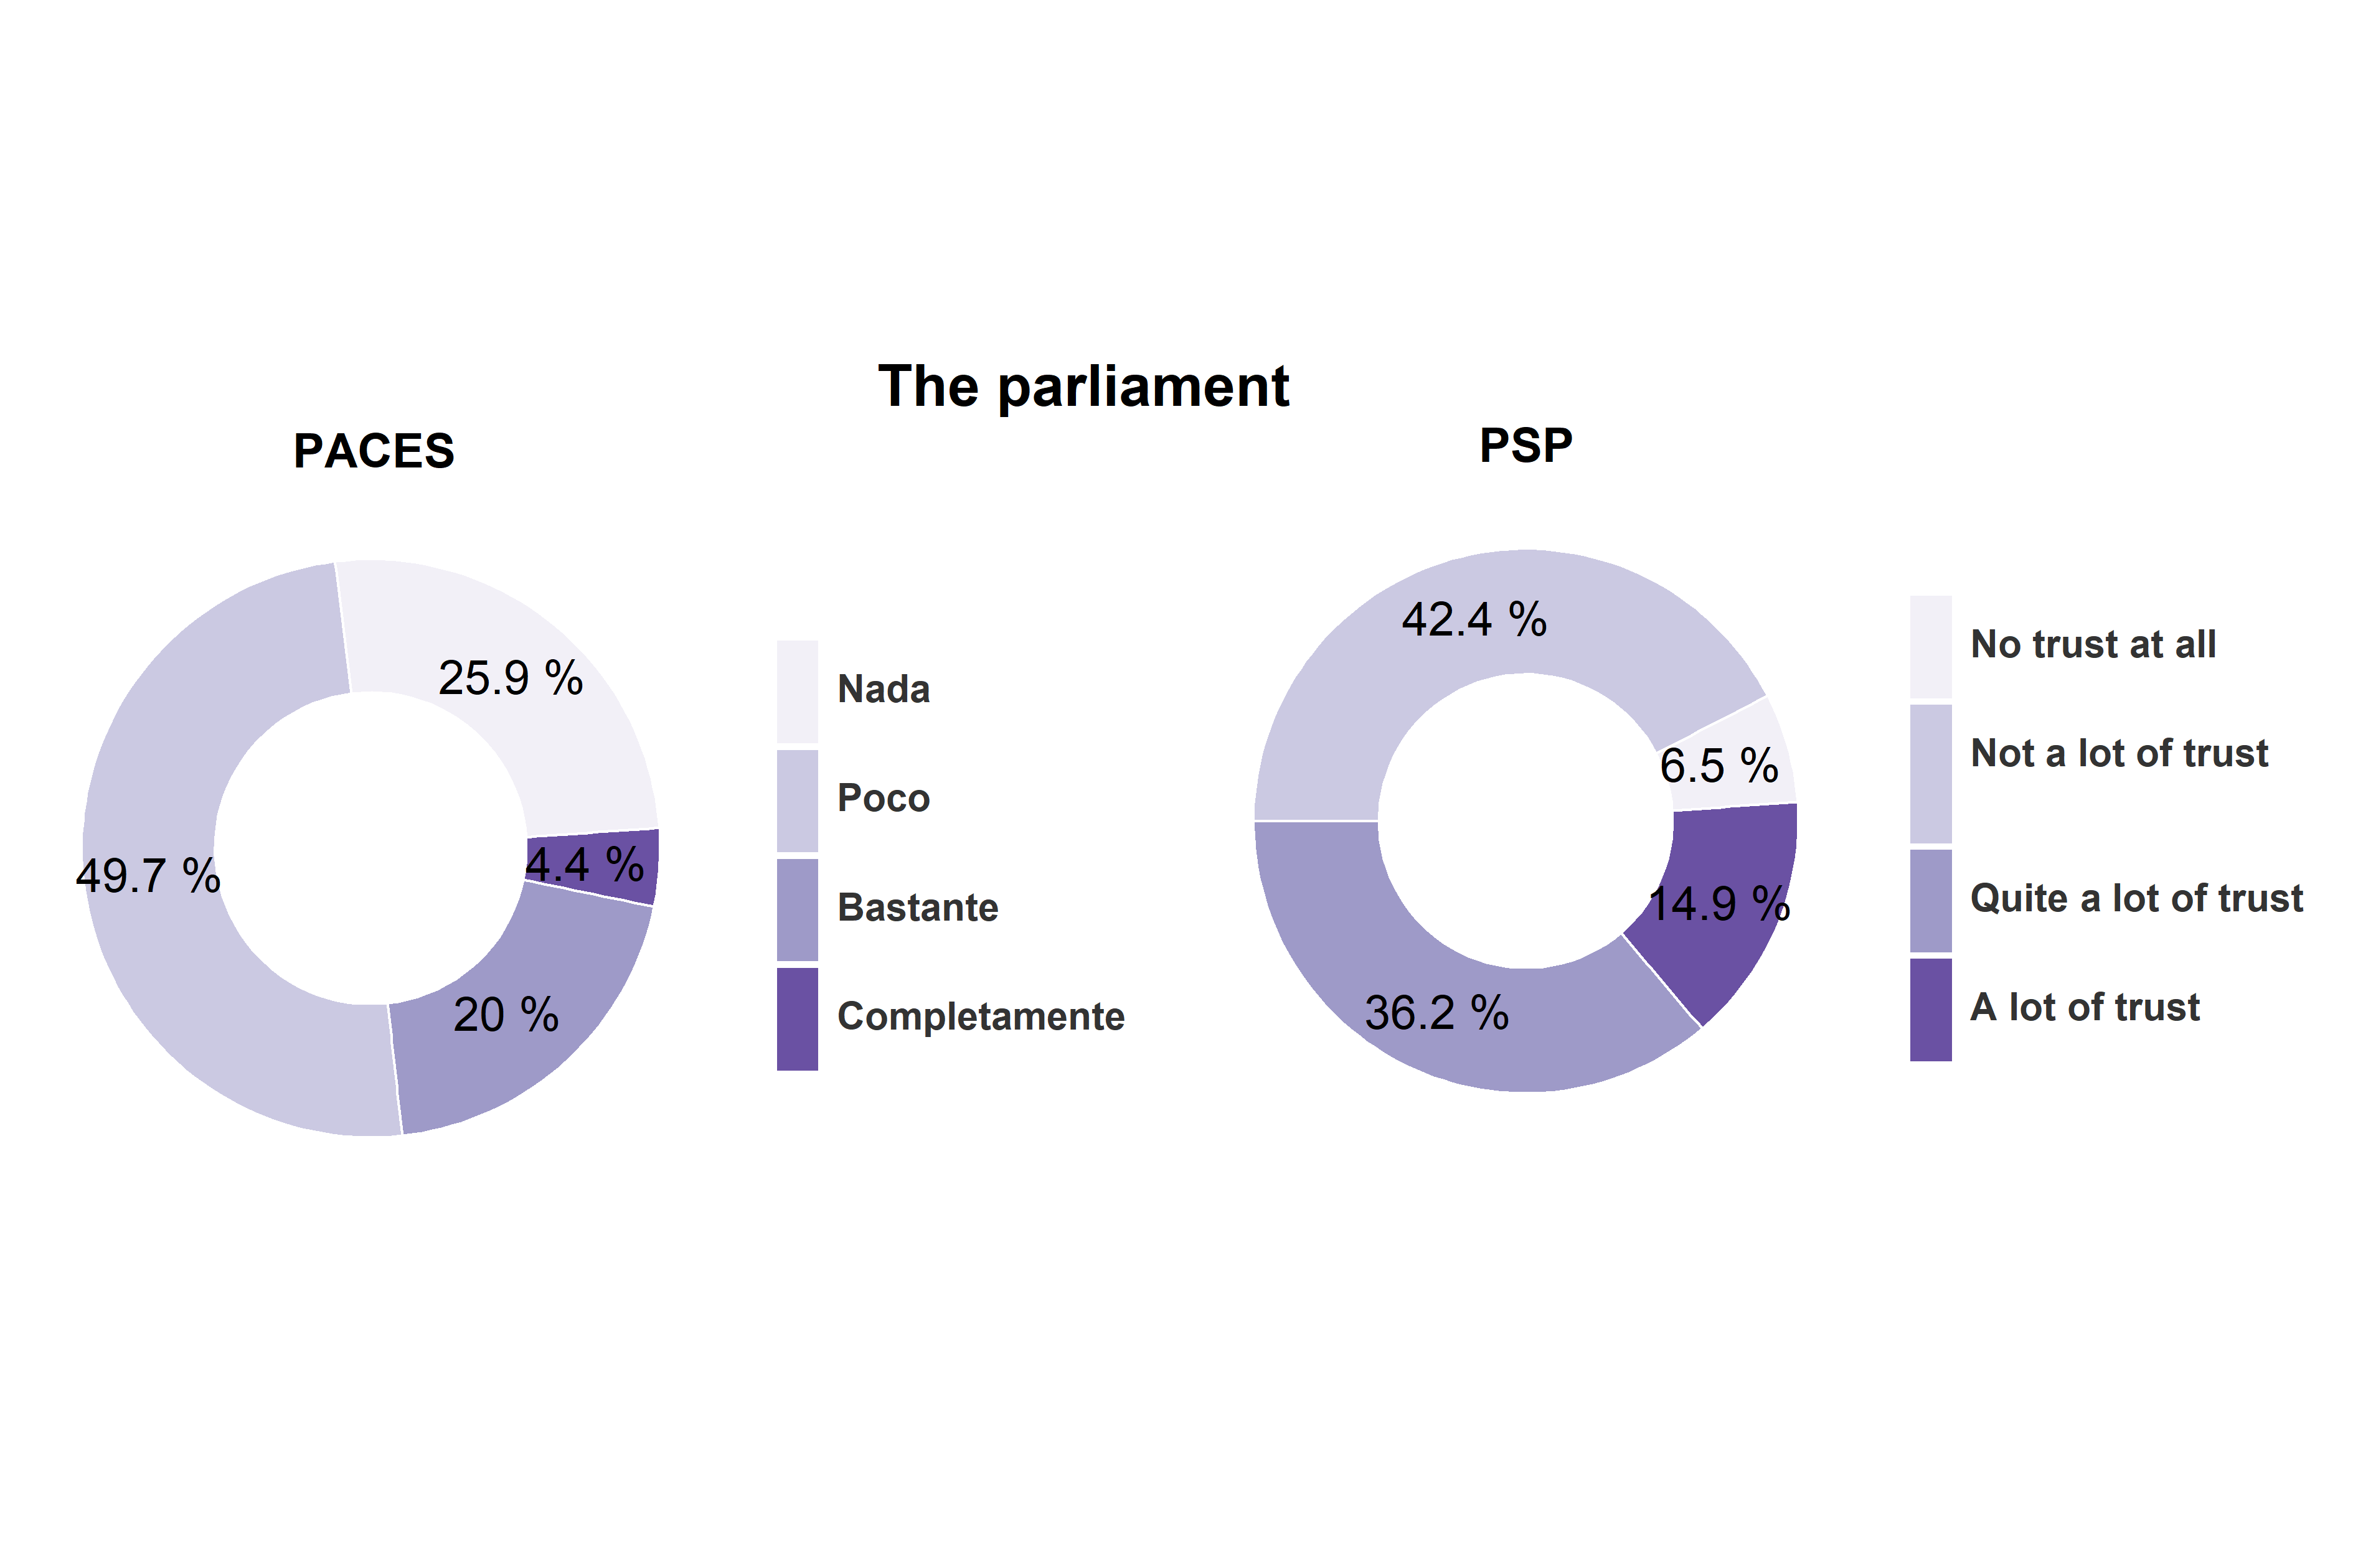
\includegraphics{output/plotru2.png}

{[}Comparar con la aceptación de los partidos en adultos{]}

\textbf{Goverment}

Los siguientes gráficos exponen el nivel de confianza de los jóvenes suecos y chilenos sobre el gobierno y el parlamento. Pese a las diferencias, se puede observar que la confianza no sobrepasa el 60\% en ninguno de los países, existiendo en ambos amplios grupos de jóvenes con baja confianza en las instituciones democráticas. Aun así, el nivel de confianza en ambas instituciones es distinto en ambos países, existe una mayor confianza en Suecia que en Chile.

Comparando la confianza en estas dos instituciones democráticas con la confianza en los partidos, que son actores relevantes en ambos poderes, se puede observar otra diferencia entre estos países. En Suecia la mitad de los jóvenes confía tanto en los partidos como en las instituciones democráticas, con un porcentaje similar de confianza sobre los partidos, el gobierno y el parlamento. Por su parte, en chile se observa una diferencia en la confianza en estas instituciones, existiendo una mayor confianza en los poderes del estado, que en los partidos que los administran.

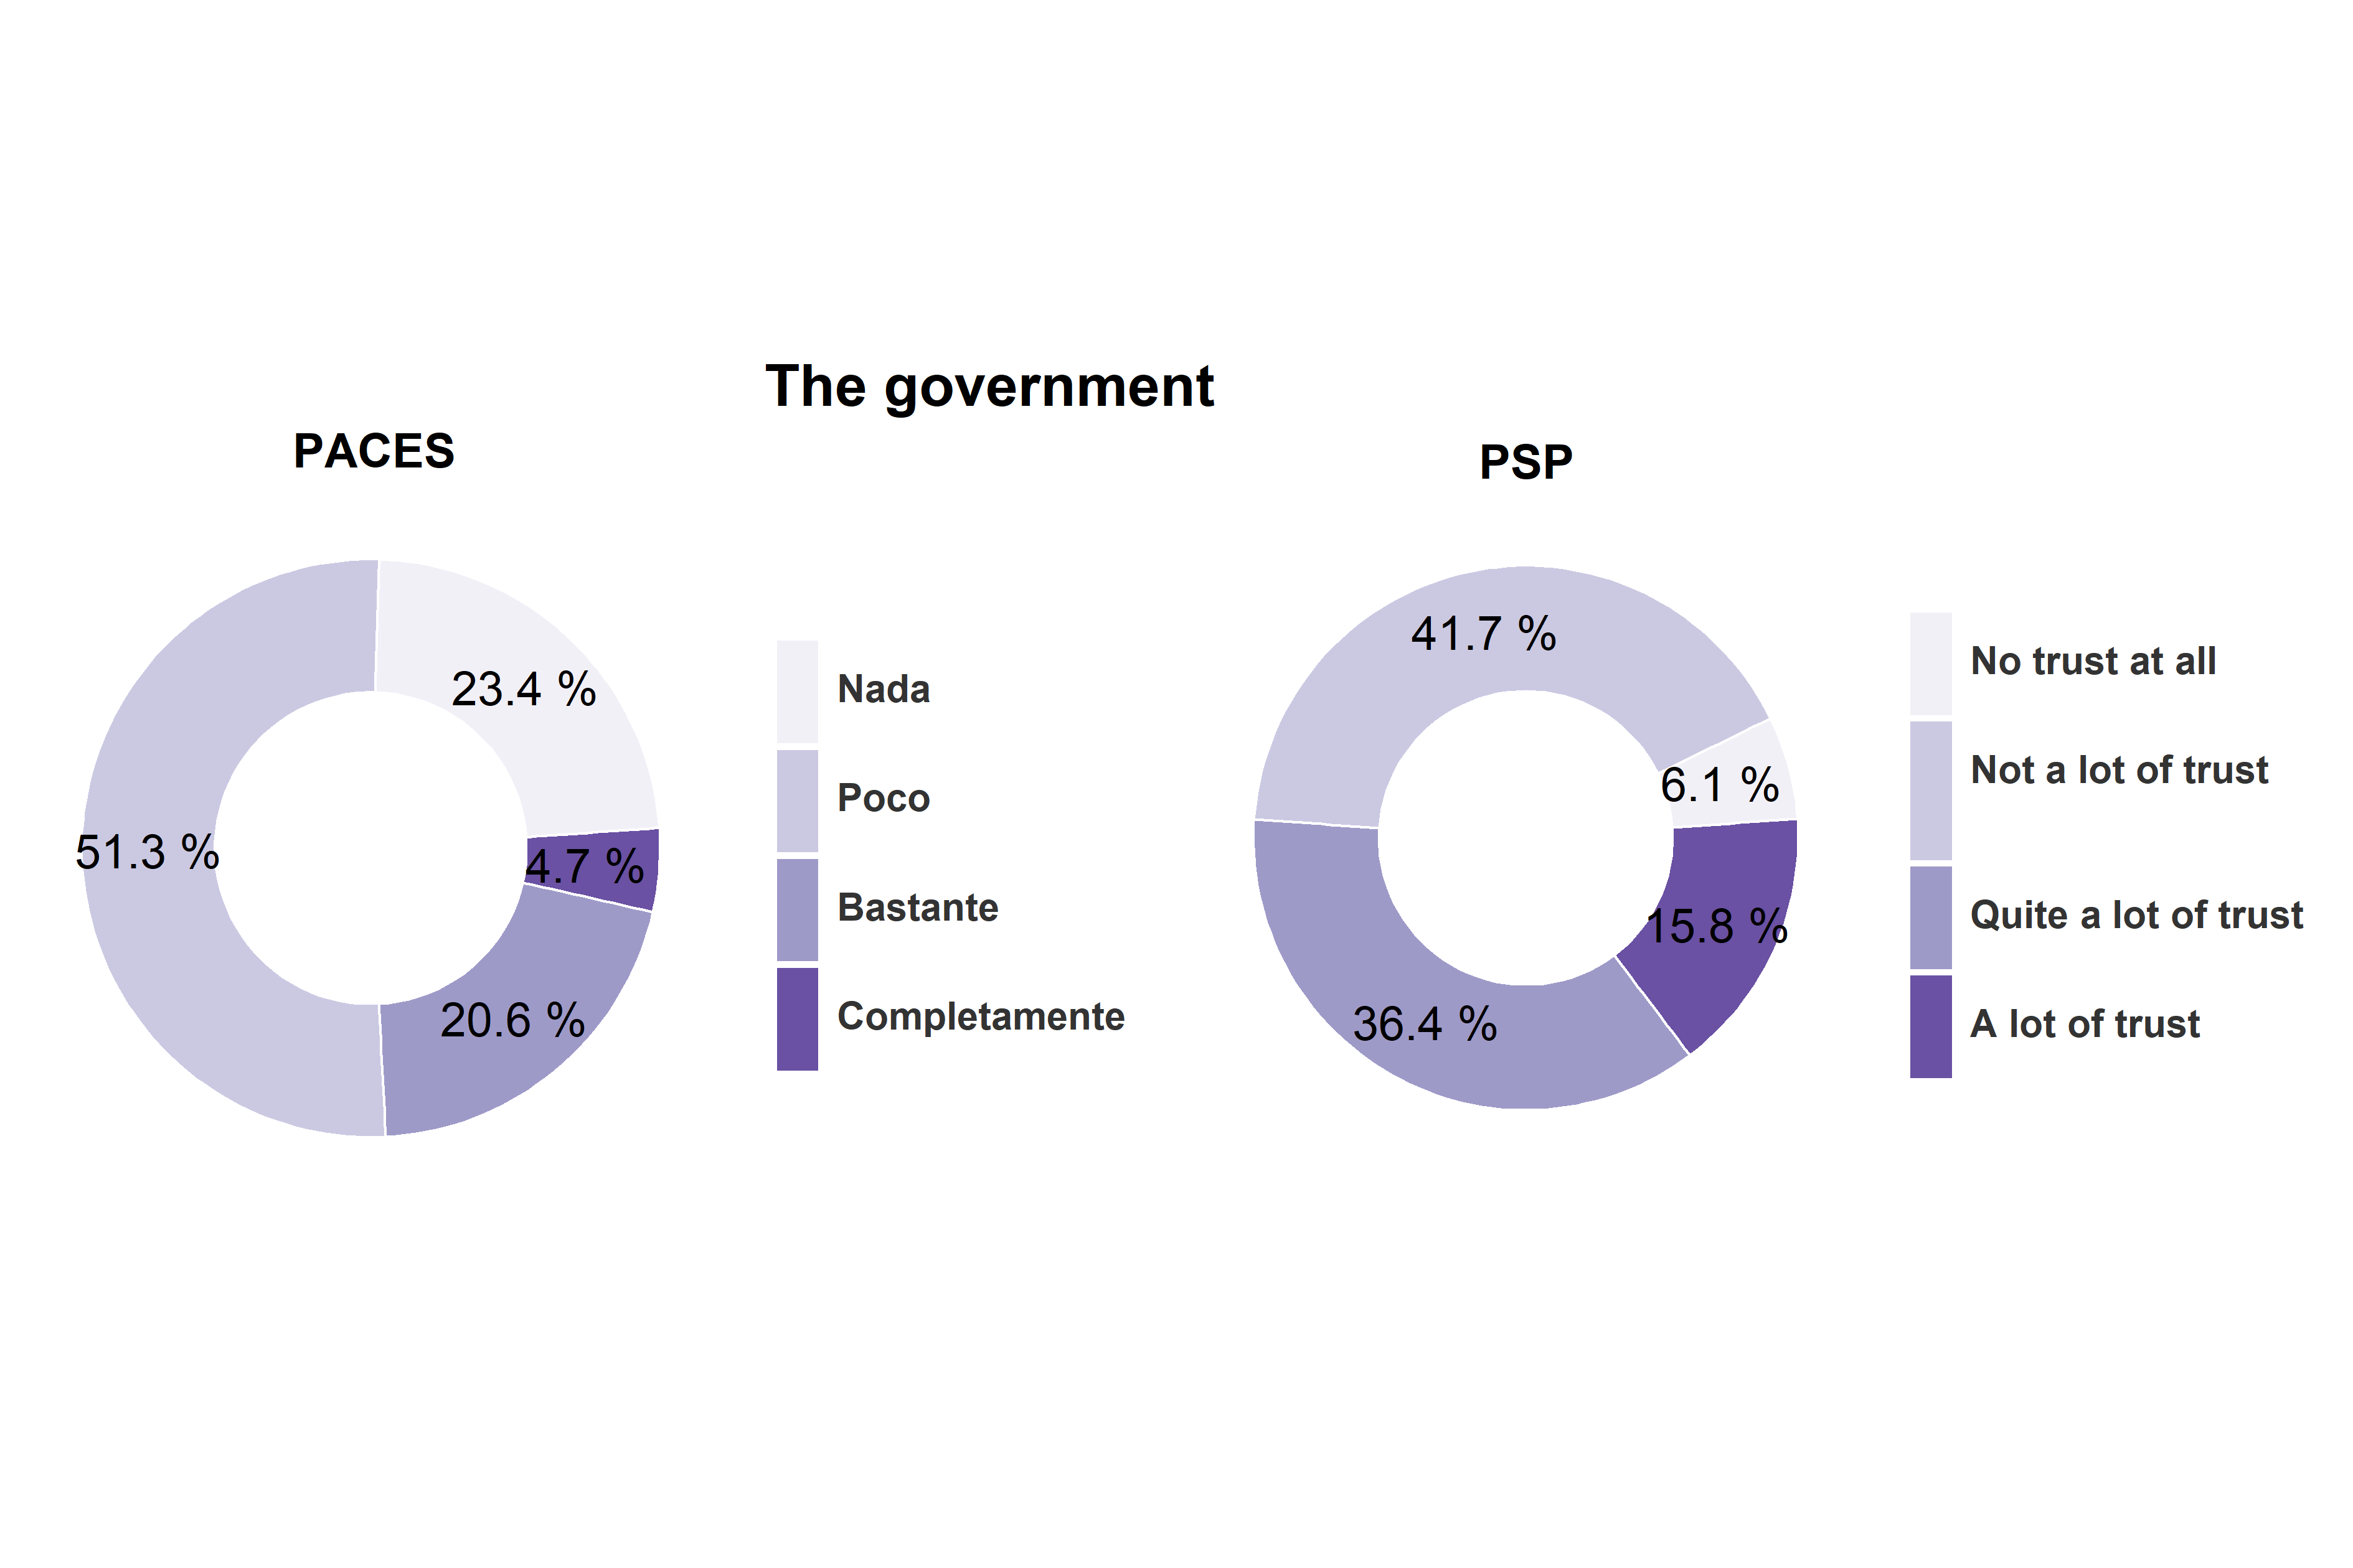
\includegraphics{output/plotru.png}

Chile tiene un sistema ejecutivo Suecia tiene un sistema legislativa. Este segundo es un incentivo al acuerdo, mientras que el otro a la competencia (política de la zancadilla de Castells en texto de red).

\textbf{\#\#\# The courts}

Este grafico expone la confianza en los tribunales, desde el punto de vista de los jóvenes de Chile y Suecia.

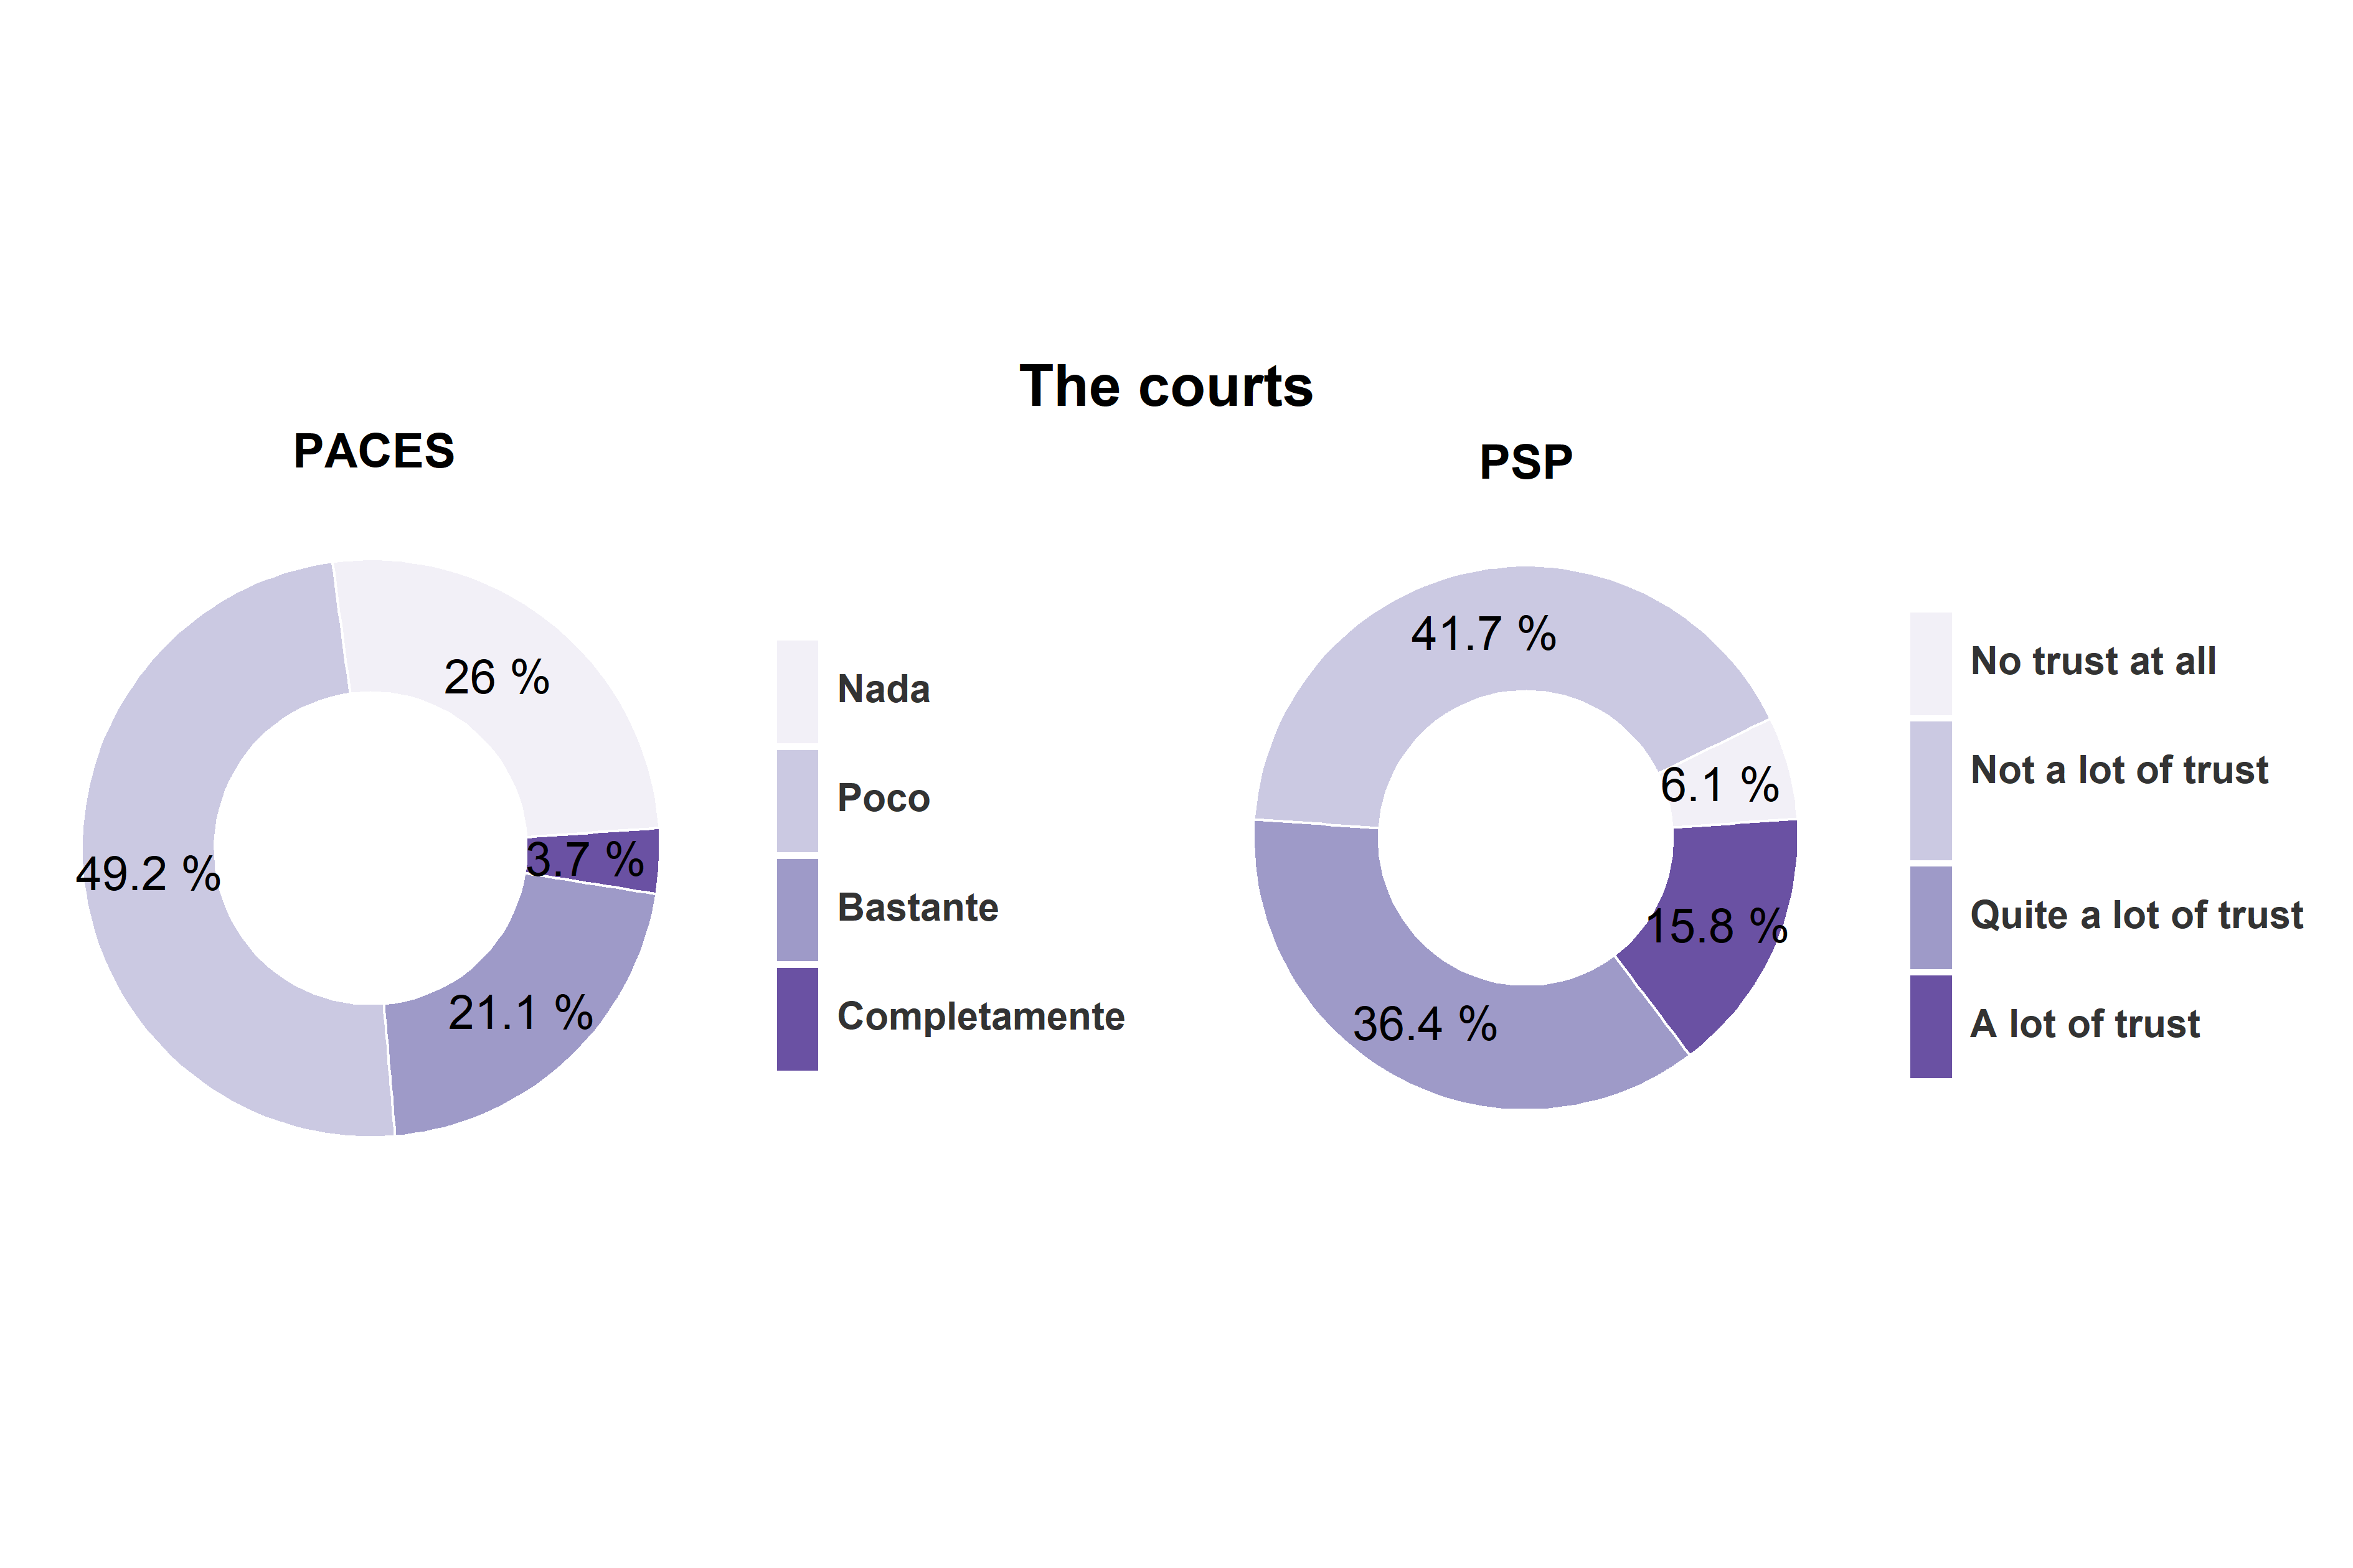
\includegraphics{output/plotru3.png}

El grafico nos sugiere nuevamente mayor confianza de los jóvenes suecos en su sistema. La proporción de jóvenes que no confía nada en los jueces de chile es un triple de lo que en Suecia.

Este resultado es consistente con la evaluación del índice de la democracia. Según este, Chile posee un sistema deficiente en torno a la garantía al derecho a la justicia, destacando la desigualdad de los tribunales. Existen casos emblemáticos que fueron muy mediáticos en chile que generaron la sensación de parcialidad por parte de los jueces {[}{]}.

\hypertarget{valores-democraticos-1}{%
\section{Valores democraticos}\label{valores-democraticos-1}}

Uno de los valores democráticos es la igualdad de derecho entre las personas. En el caso de Chile, la igualdad de derechos tiene un rol importante en los planes de Educación cívica y formación ciudadana (). La igualdad de derechos implica la no discriminación por razones arbitrarias como sexo u origen. Al respecto los siguientes gráficos nos muestran la opinión de los jóvenes frente a la igualdad de derecho entre géneros y con los inmigrantes.

\hypertarget{igualdad-de-derechos-con-inmigrantes}{%
\subsubsection{Igualdad de derechos con inmigrantes}\label{igualdad-de-derechos-con-inmigrantes}}

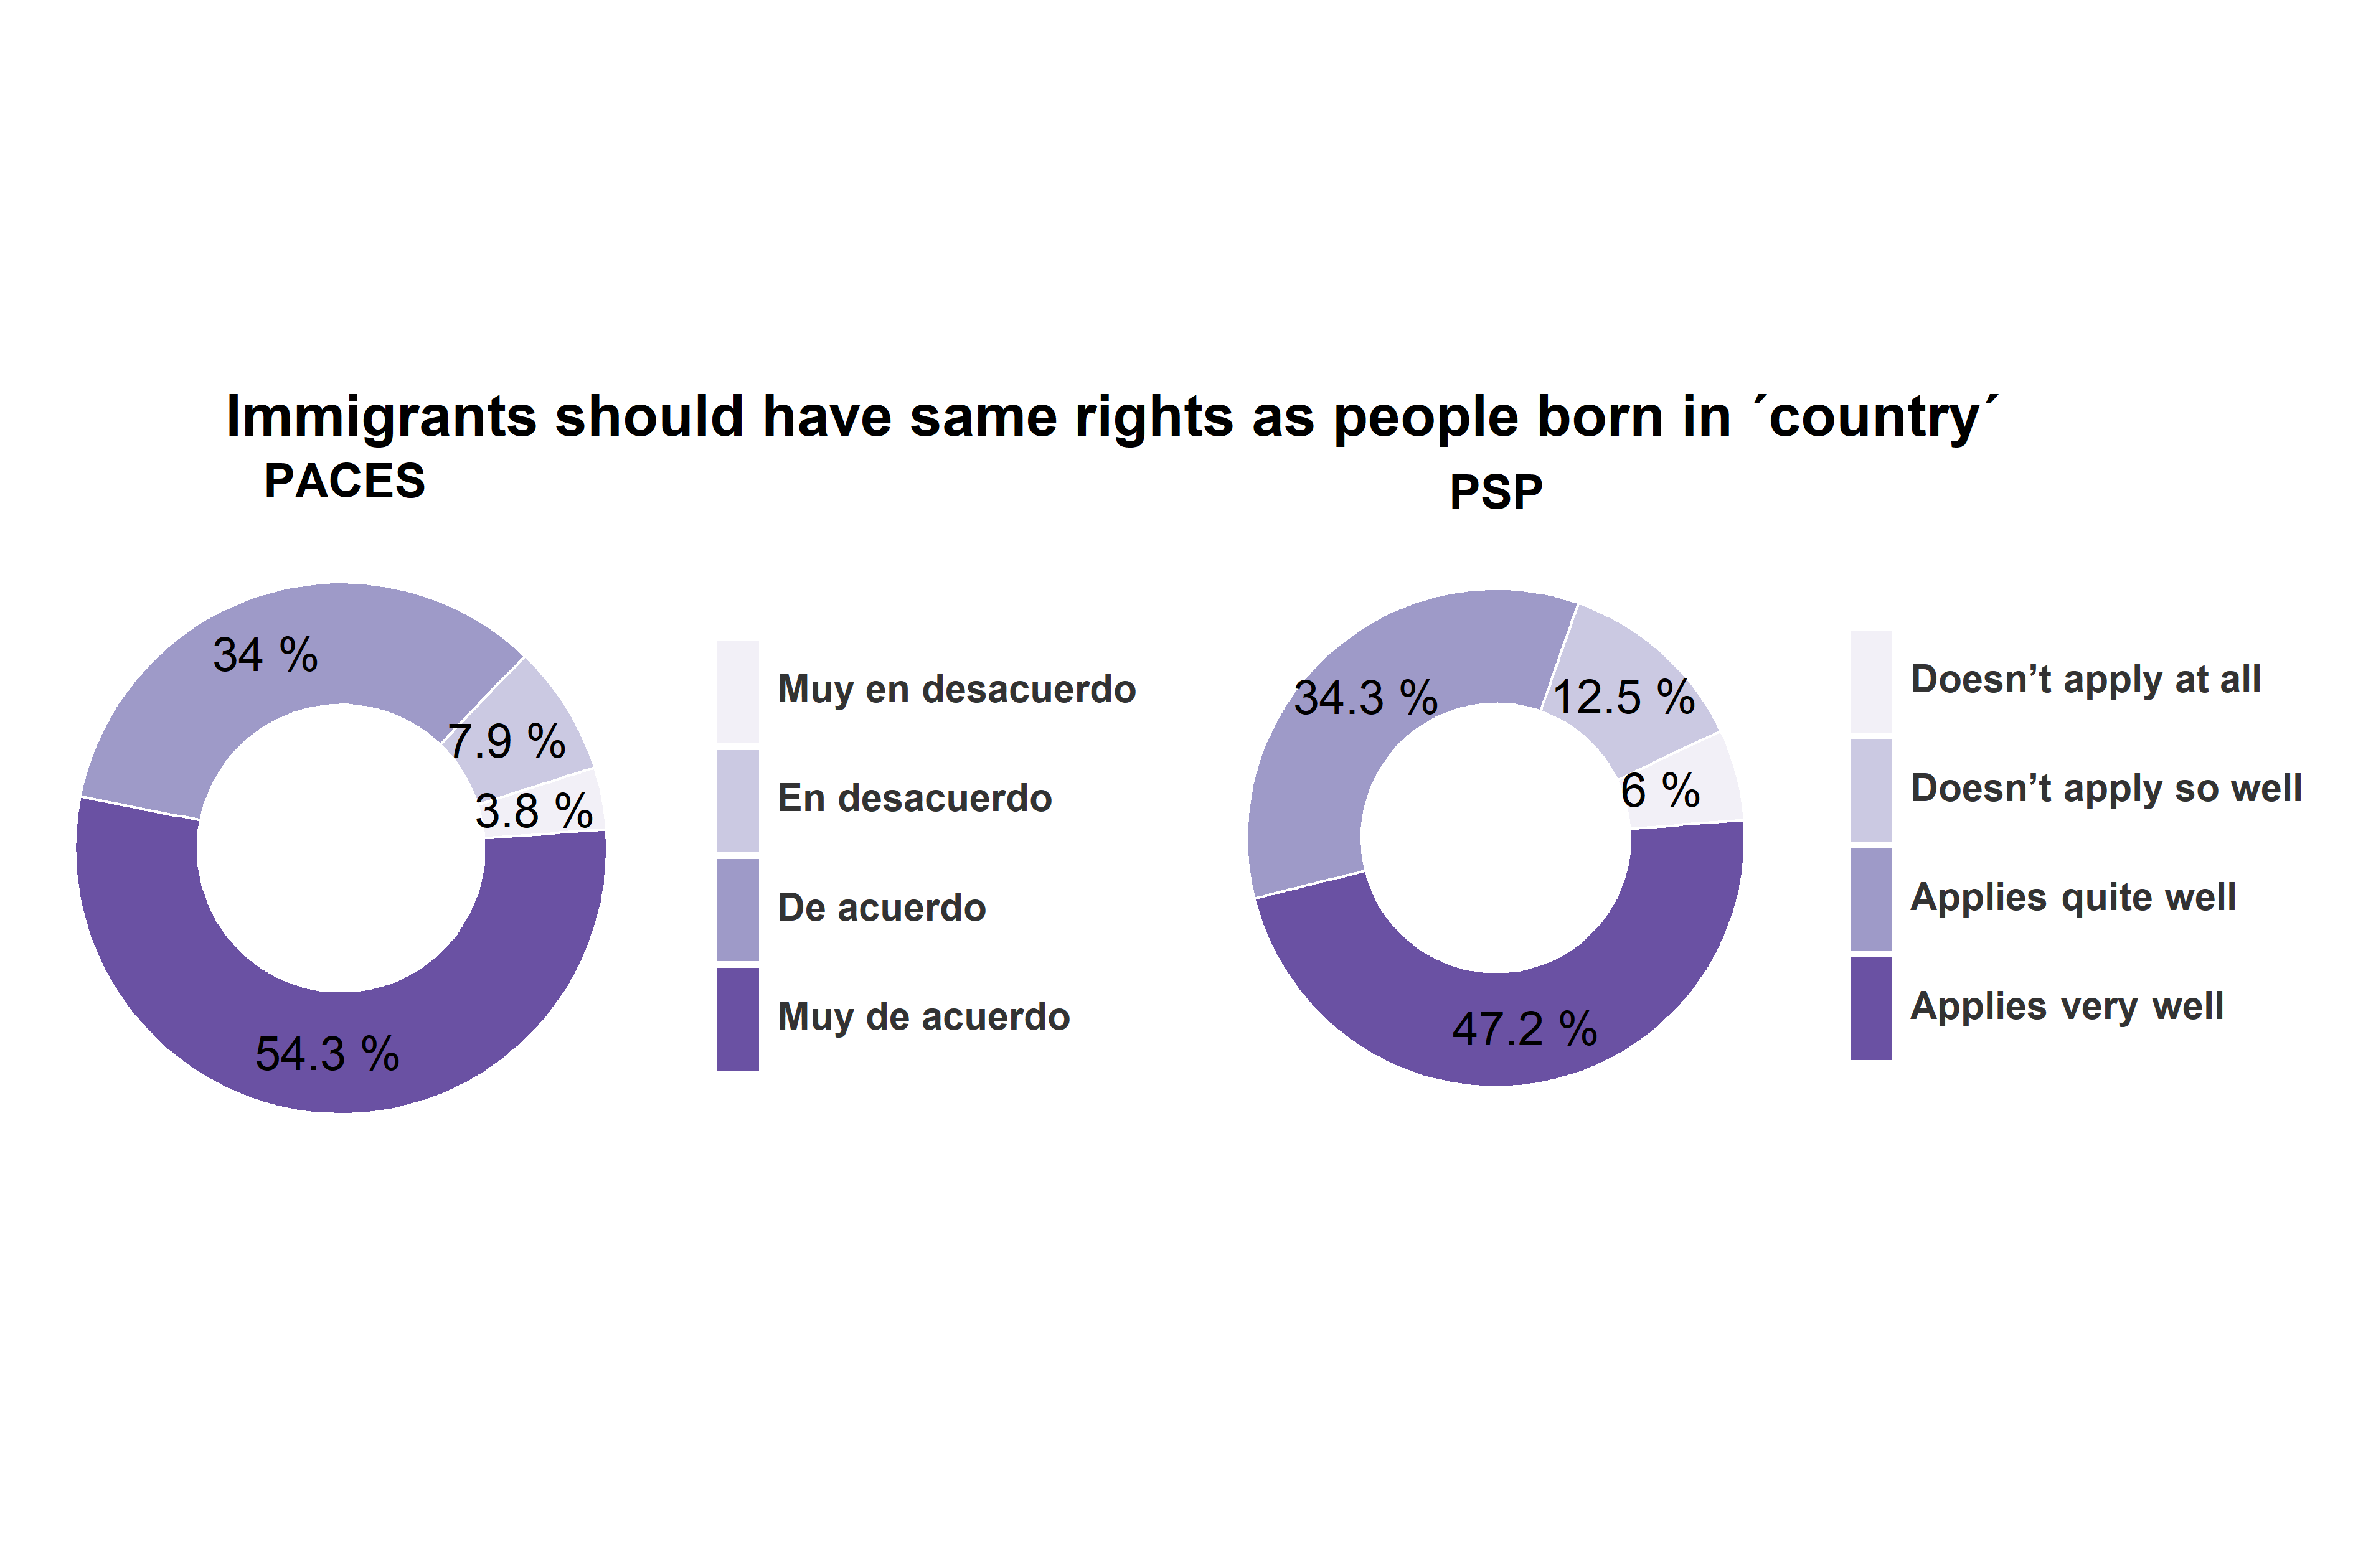
\includegraphics{output/plotinm2.png}

Los resultados de ambos gráficos permiten apreciar que no existe una diferencia valórica entre los jóvenes suecos y chilenos respecto a la igualdad de derechos. Más bien los patrones de respuesta son bastante similares. Existen pequeñas diferencias según las cuales en chile los jóvenes son levemente más propensos a justificar la desigualdad de género, mientras los jóvenes de Suecia más propensos a justificar la desigualdad en derechos con los inmigrantes.

\hypertarget{igualdad-de-derechos-entre-generos}{%
\subsubsection{Igualdad de derechos entre generos}\label{igualdad-de-derechos-entre-generos}}

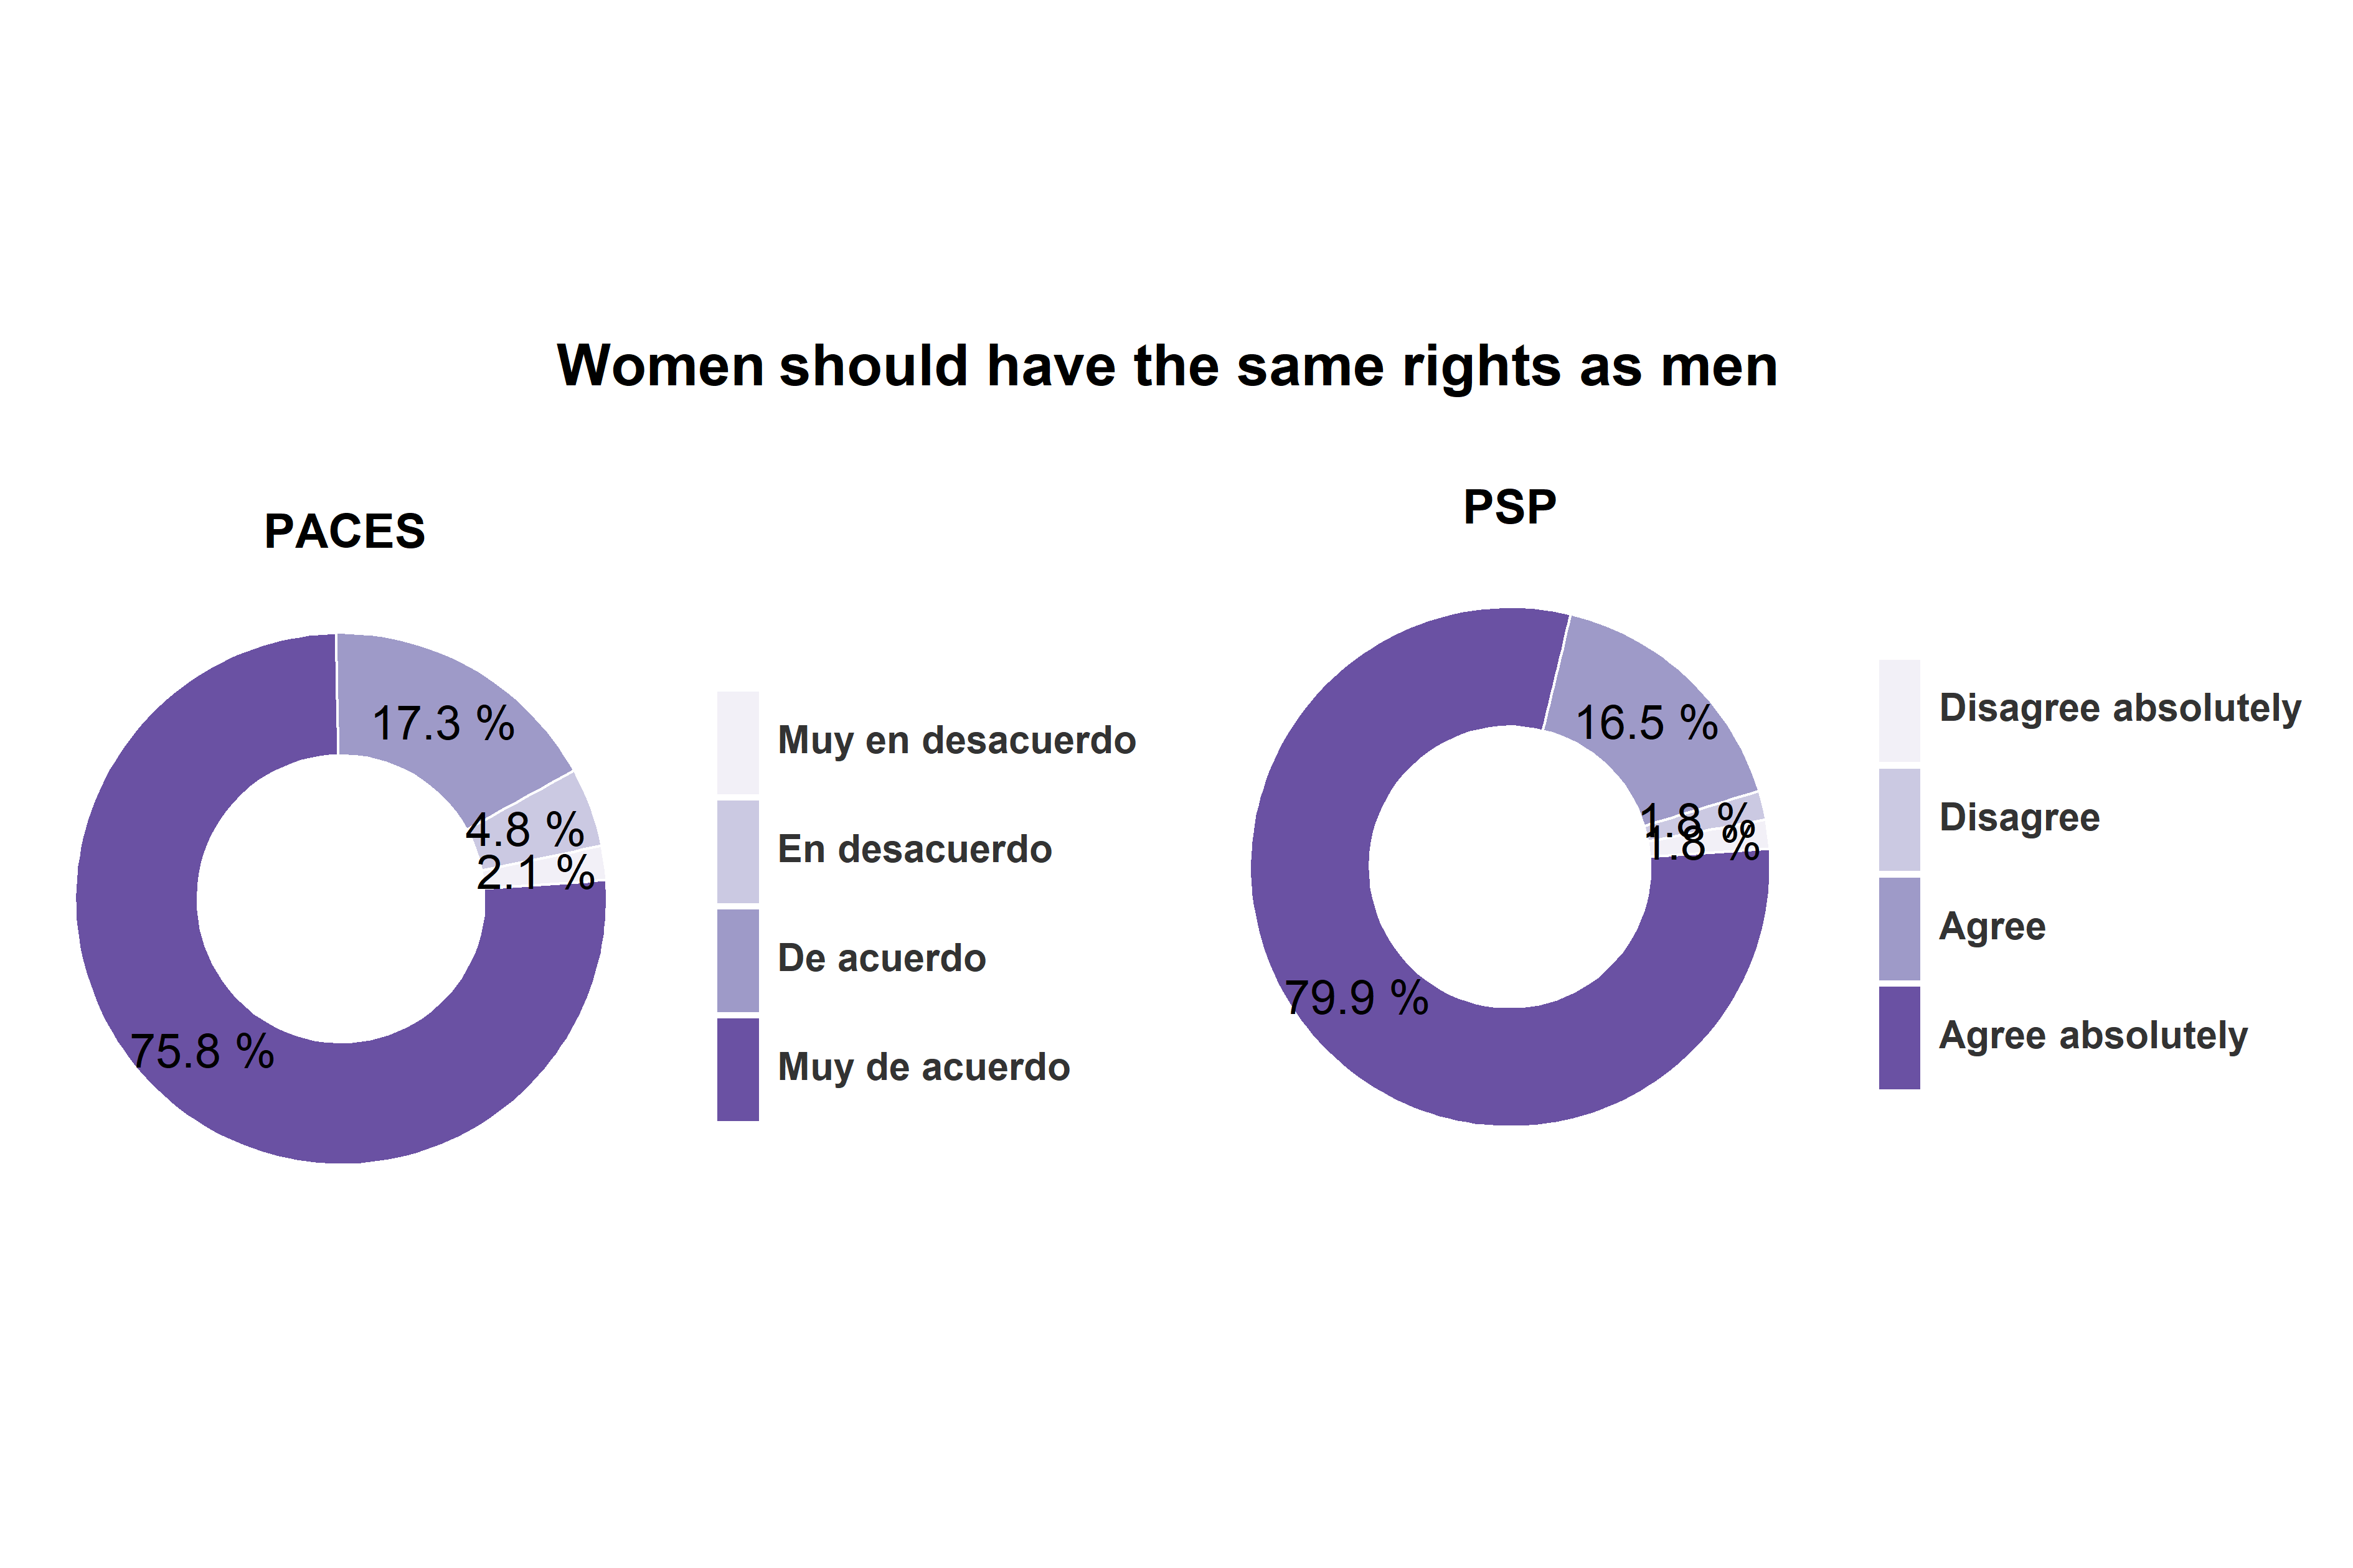
\includegraphics{output/plotdem.png}

\hypertarget{idea-de-un-buen-ciudadano}{%
\subsection{Idea de un buen ciudadano}\label{idea-de-un-buen-ciudadano}}

\hypertarget{participaciuxf3n}{%
\section{Participación}\label{participaciuxf3n}}

\hypertarget{participaciuxf3n-en-la-escuela}{%
\subsubsection{Participación en la escuela}\label{participaciuxf3n-en-la-escuela}}

\textbf{Youth school political participation}

\textbf{Been a member of the student council}

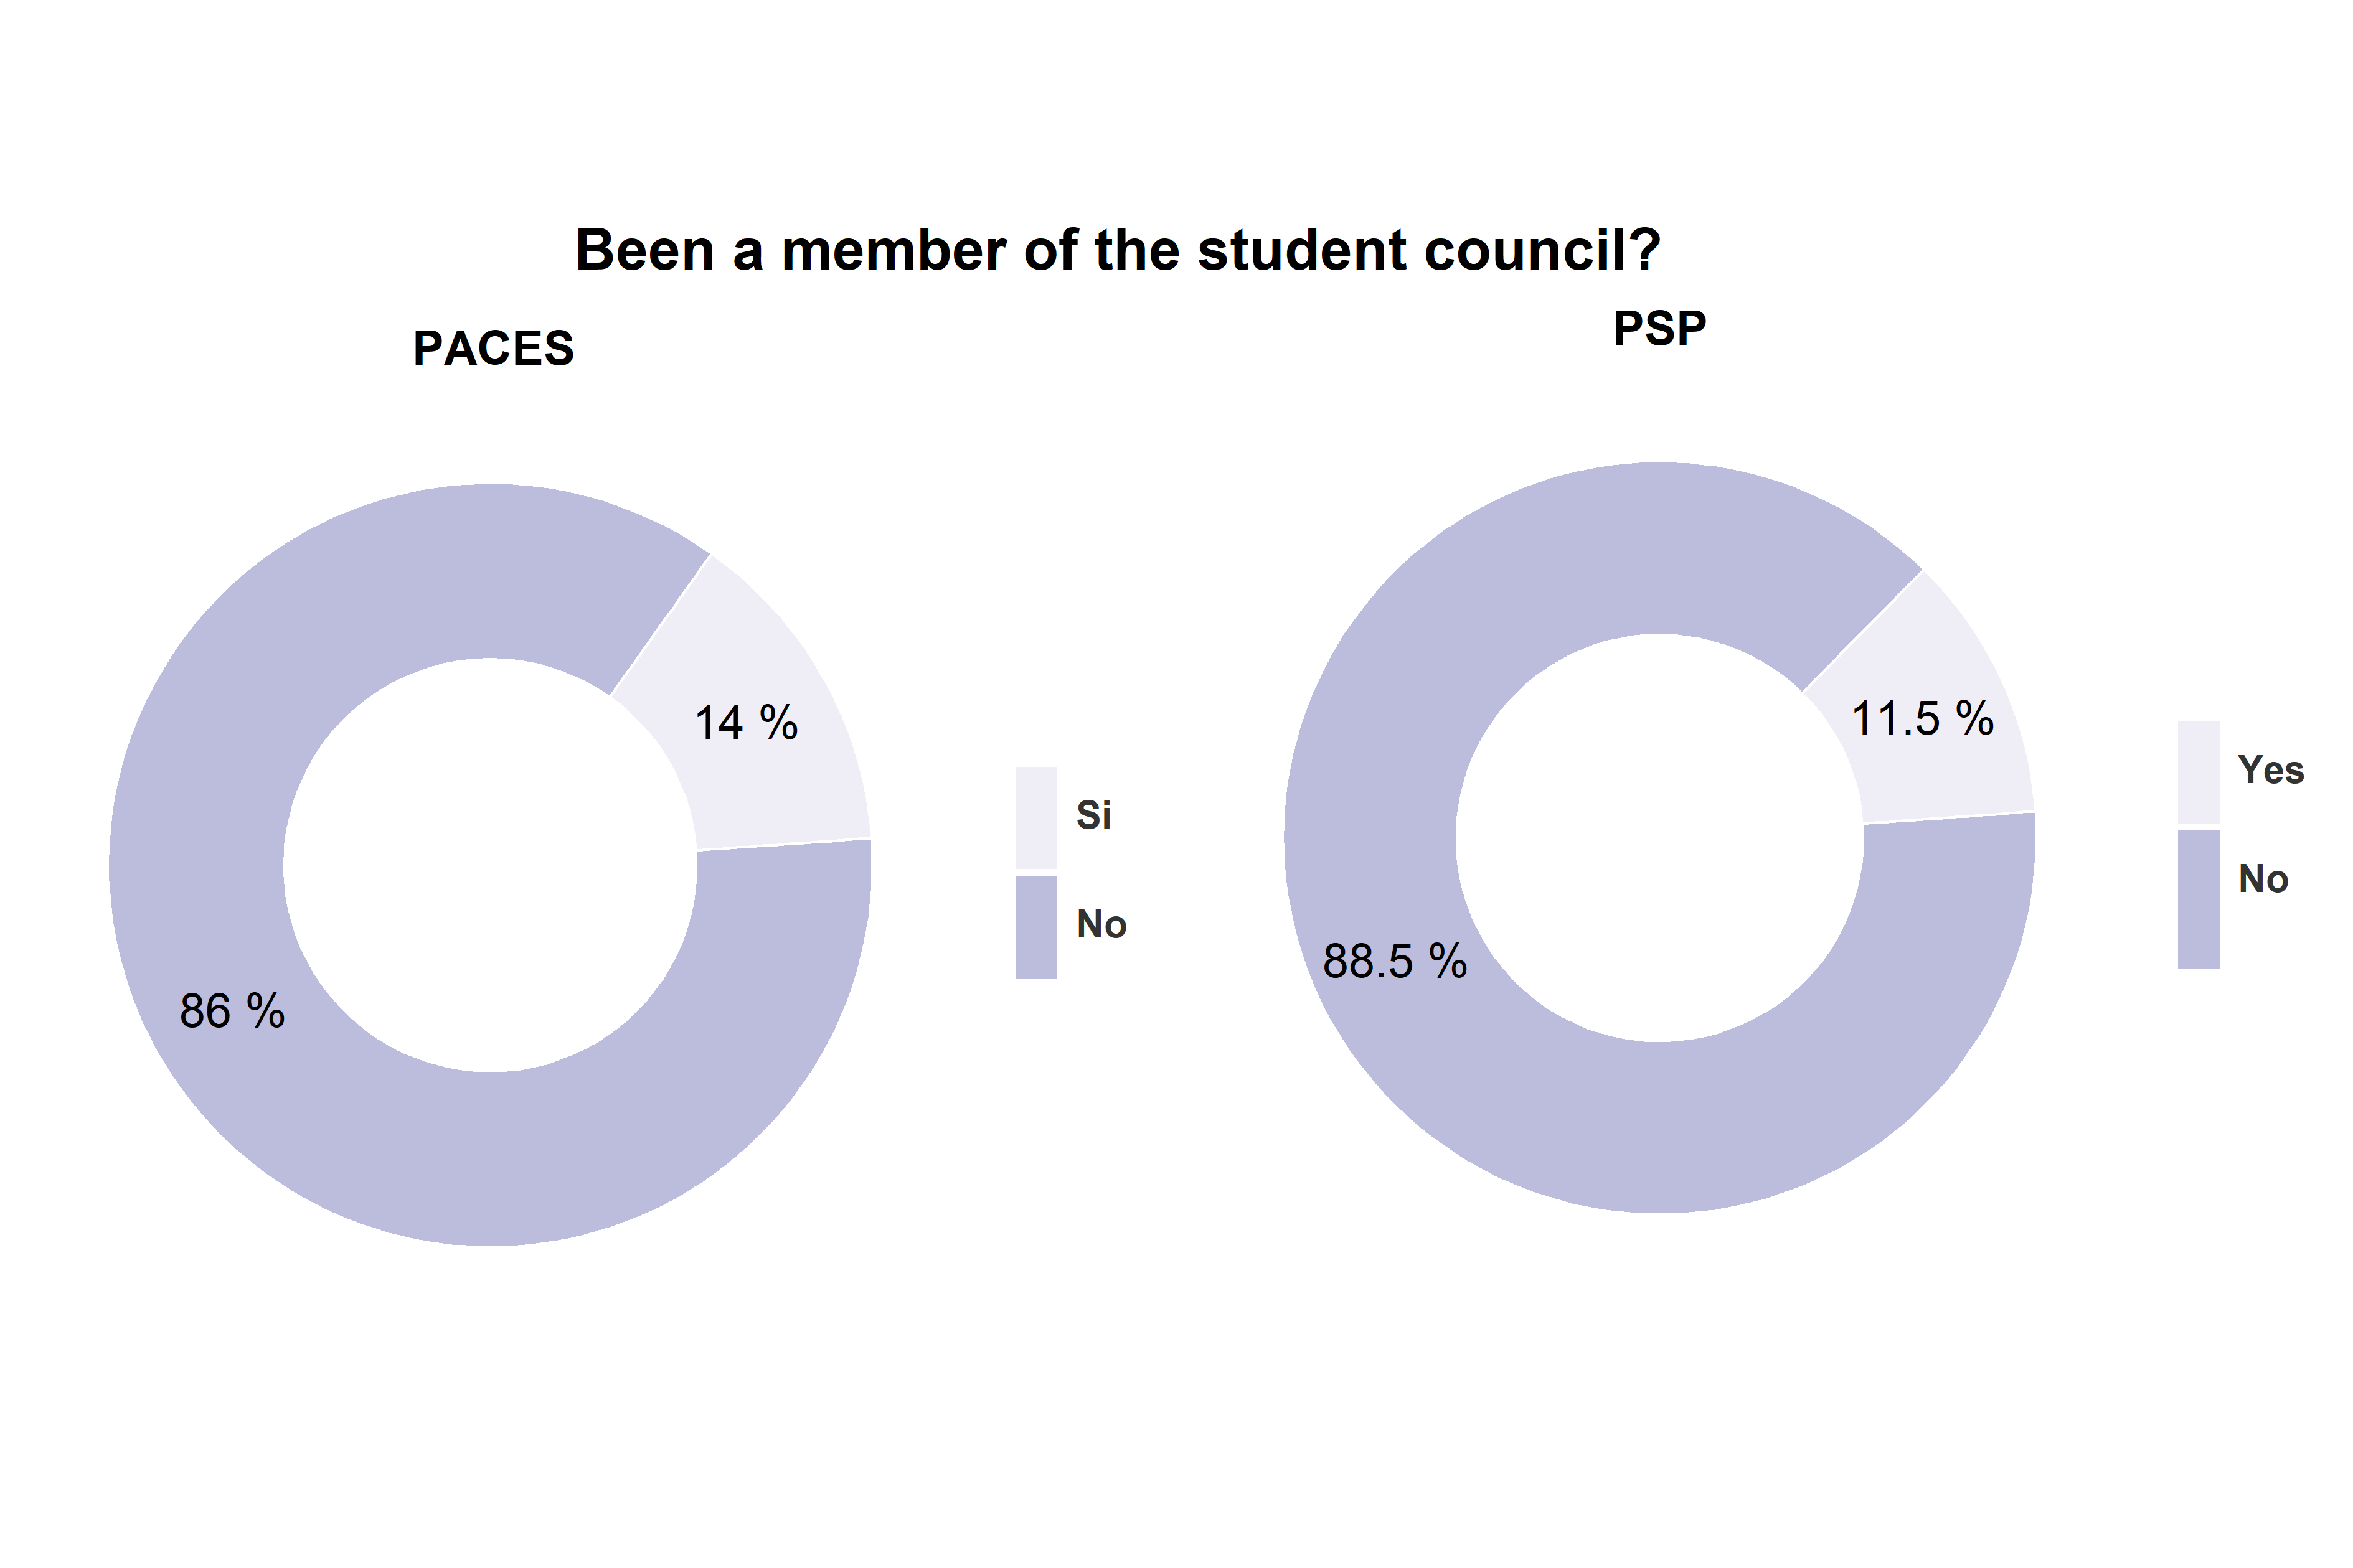
\includegraphics{output/plottr.png}

\textbf{Taken an active role at a students' meeting?}

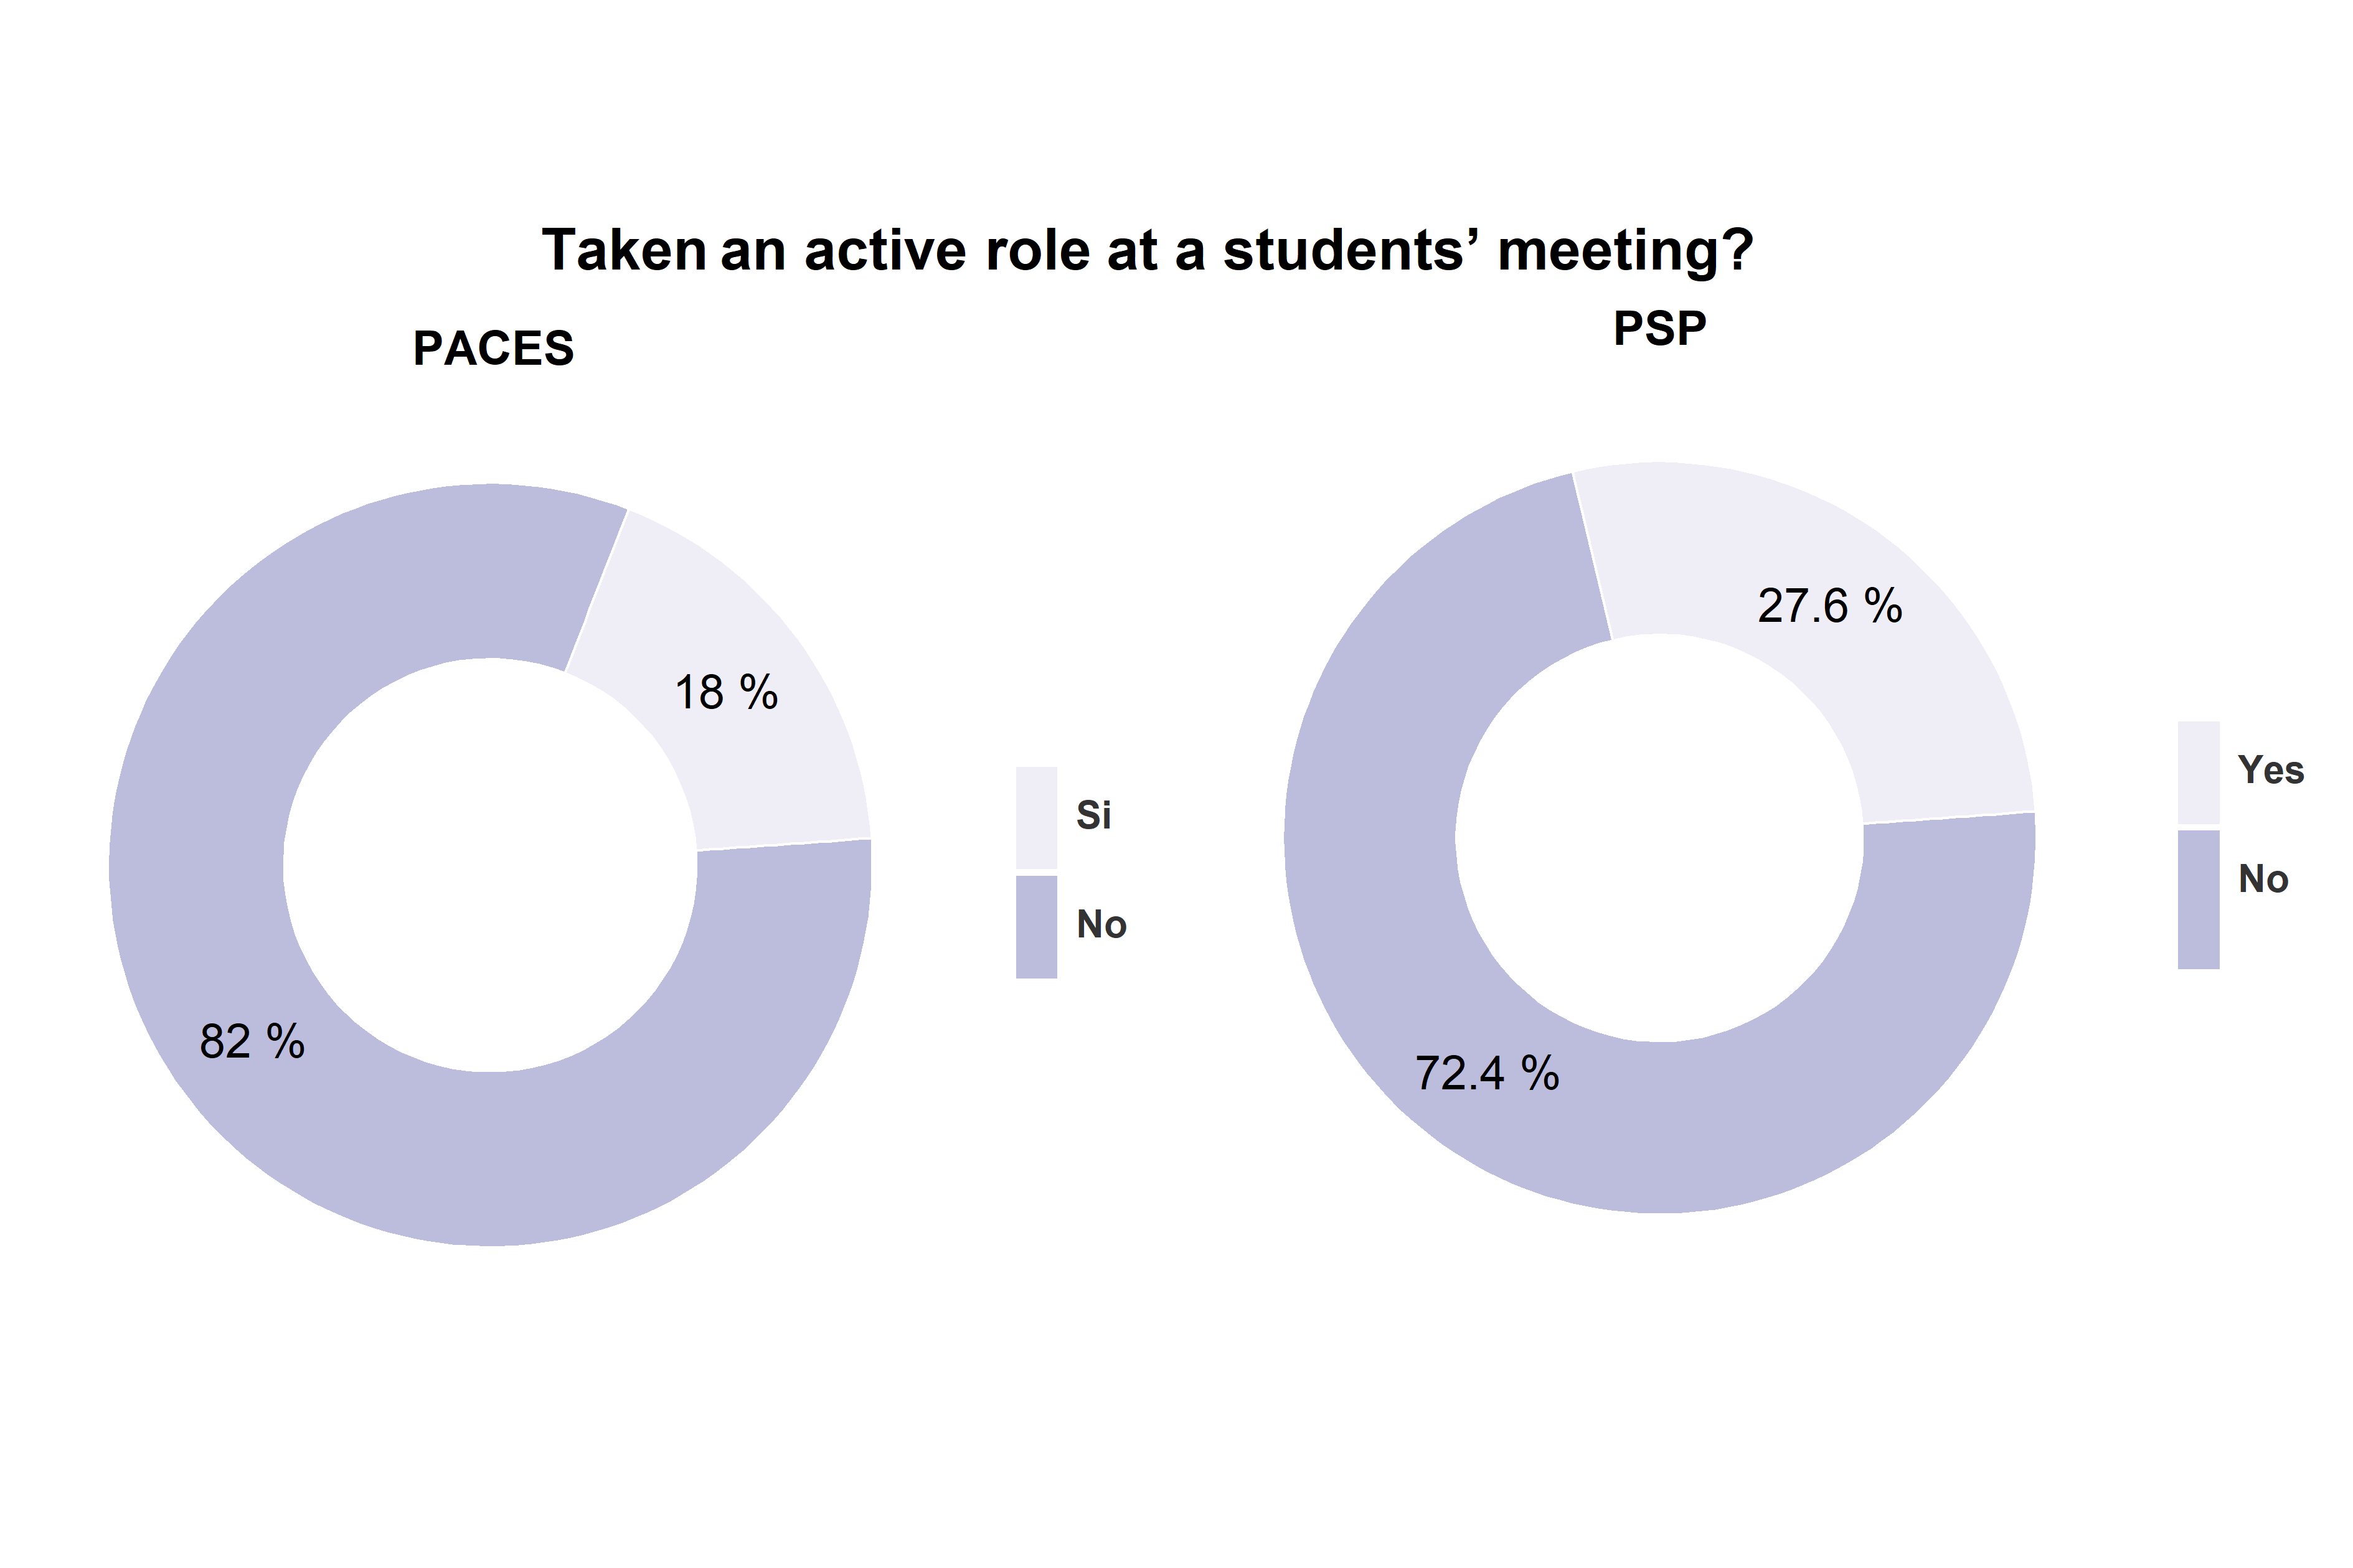
\includegraphics{output/plottr2.png}

\textbf{Voted in a school election?}

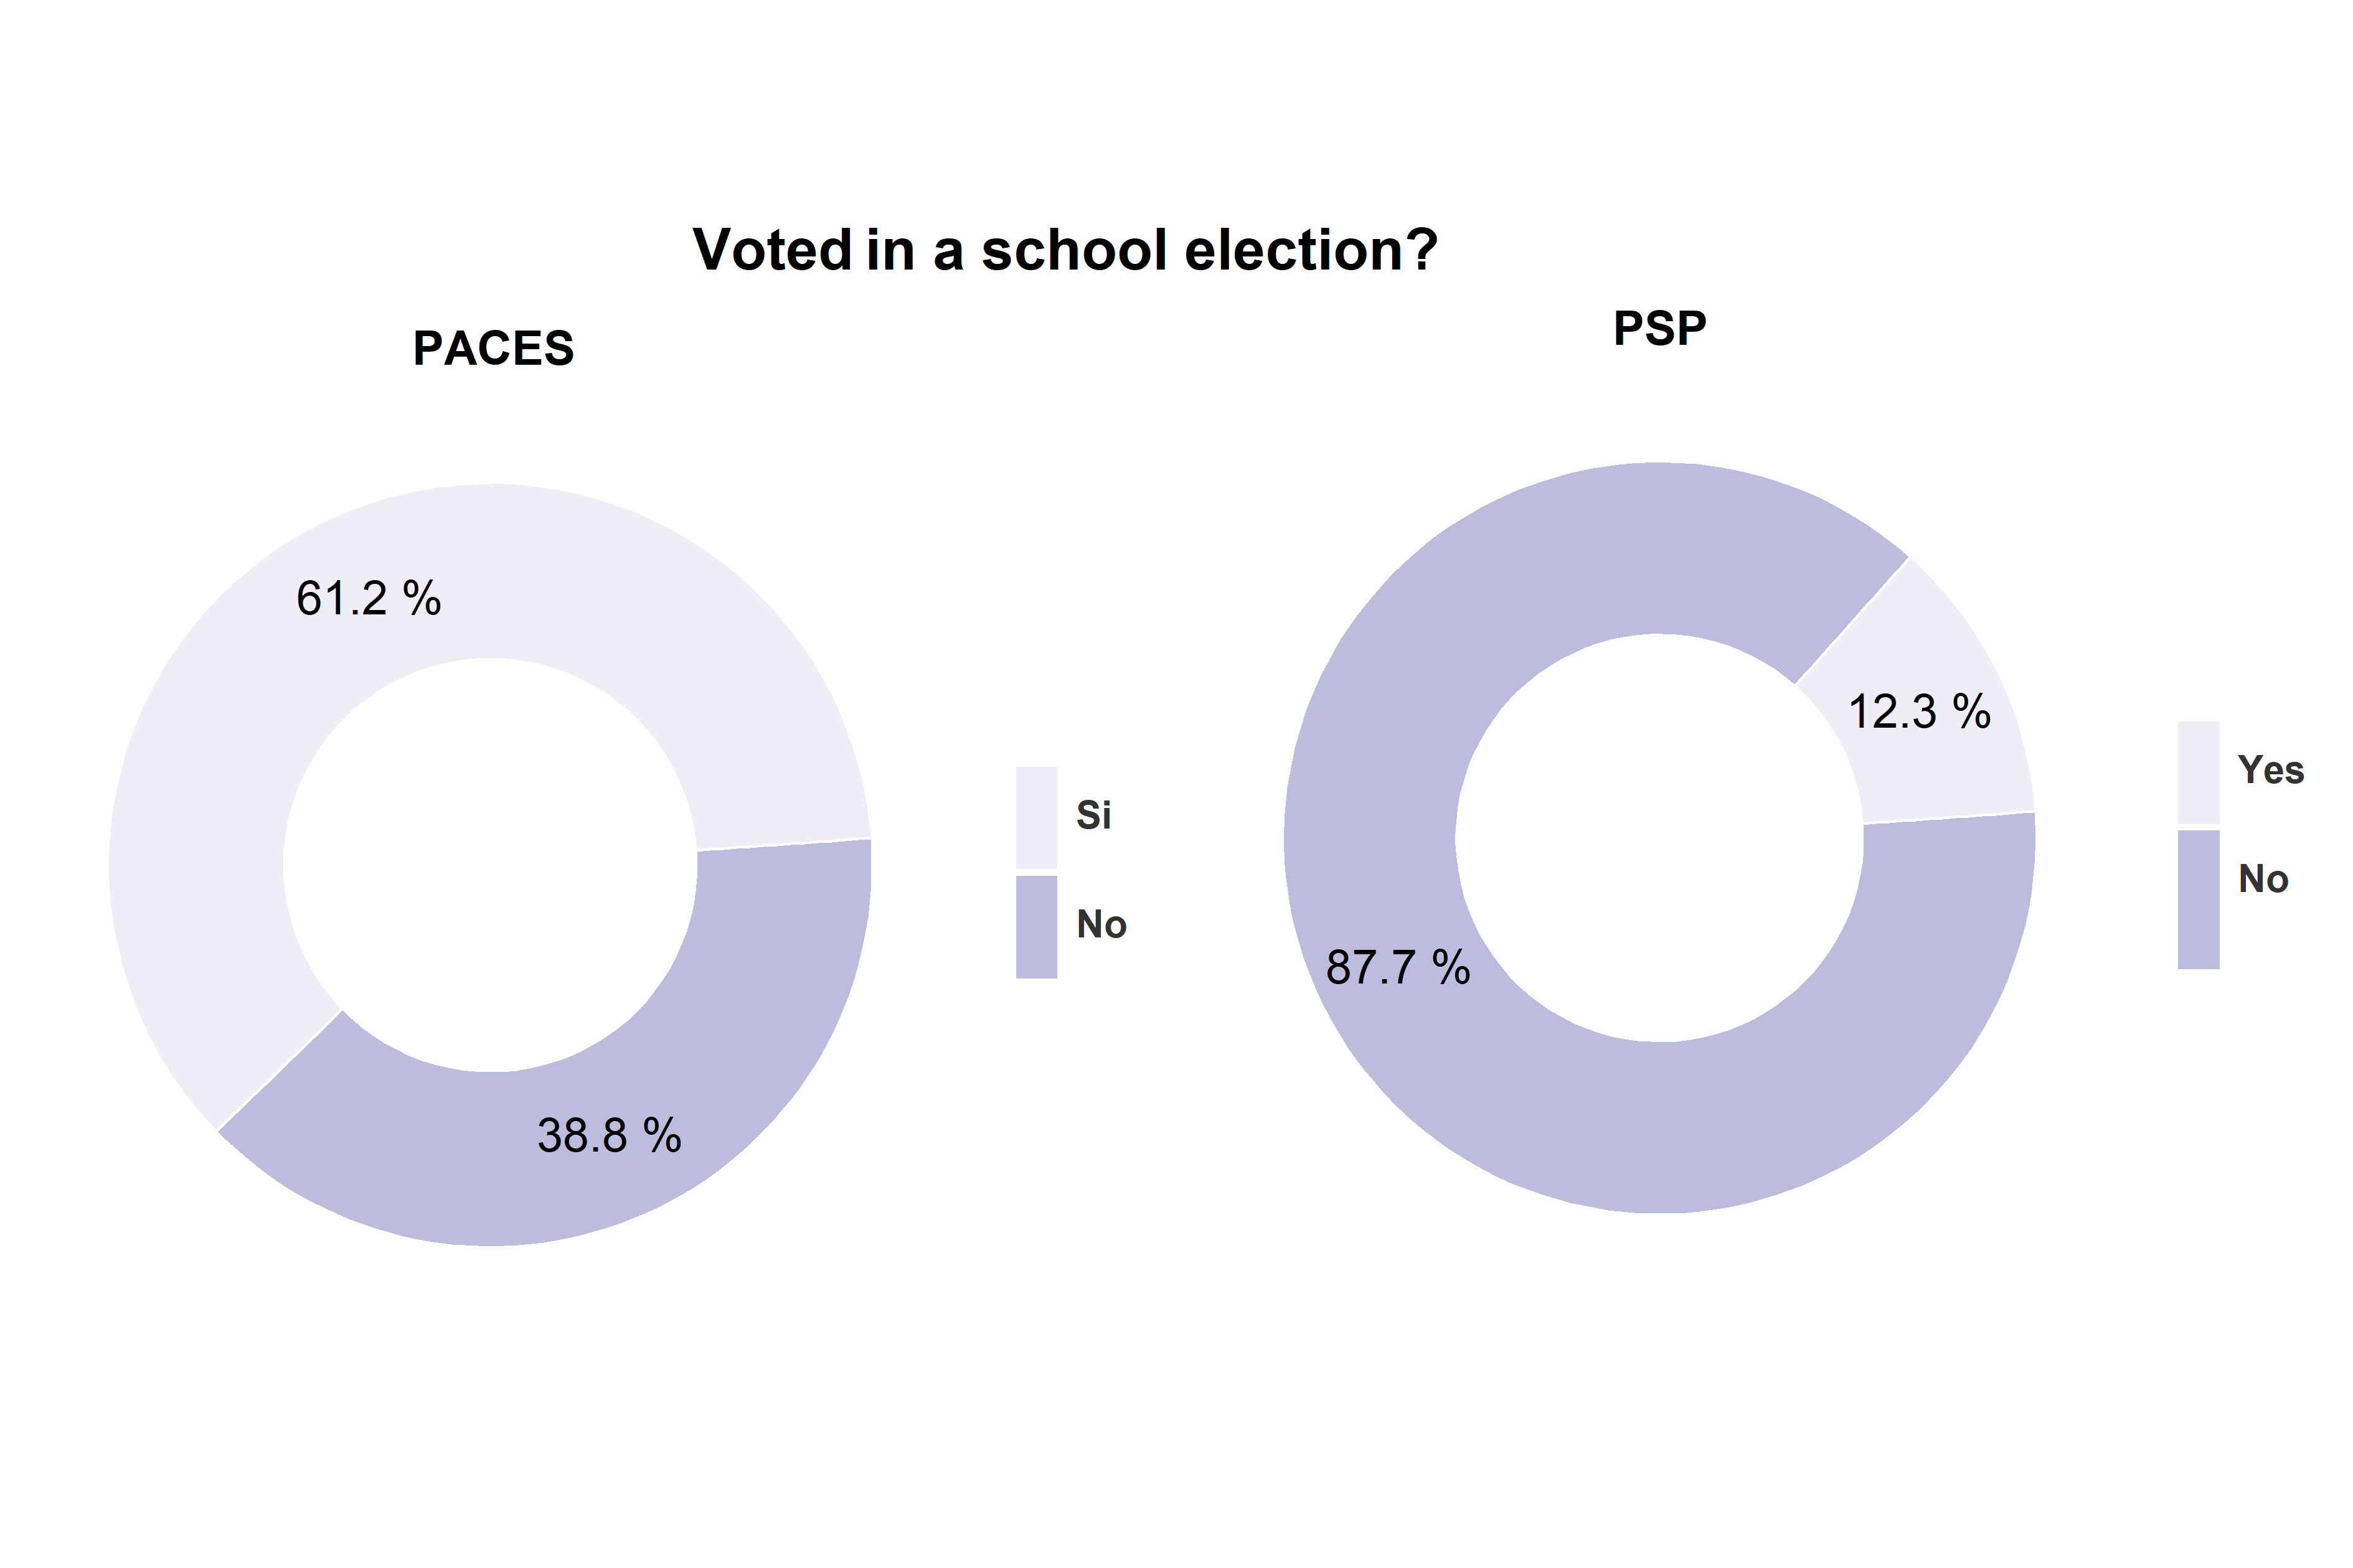
\includegraphics{output/plottr3.png}

\textbf{Participated in a protest at school?}

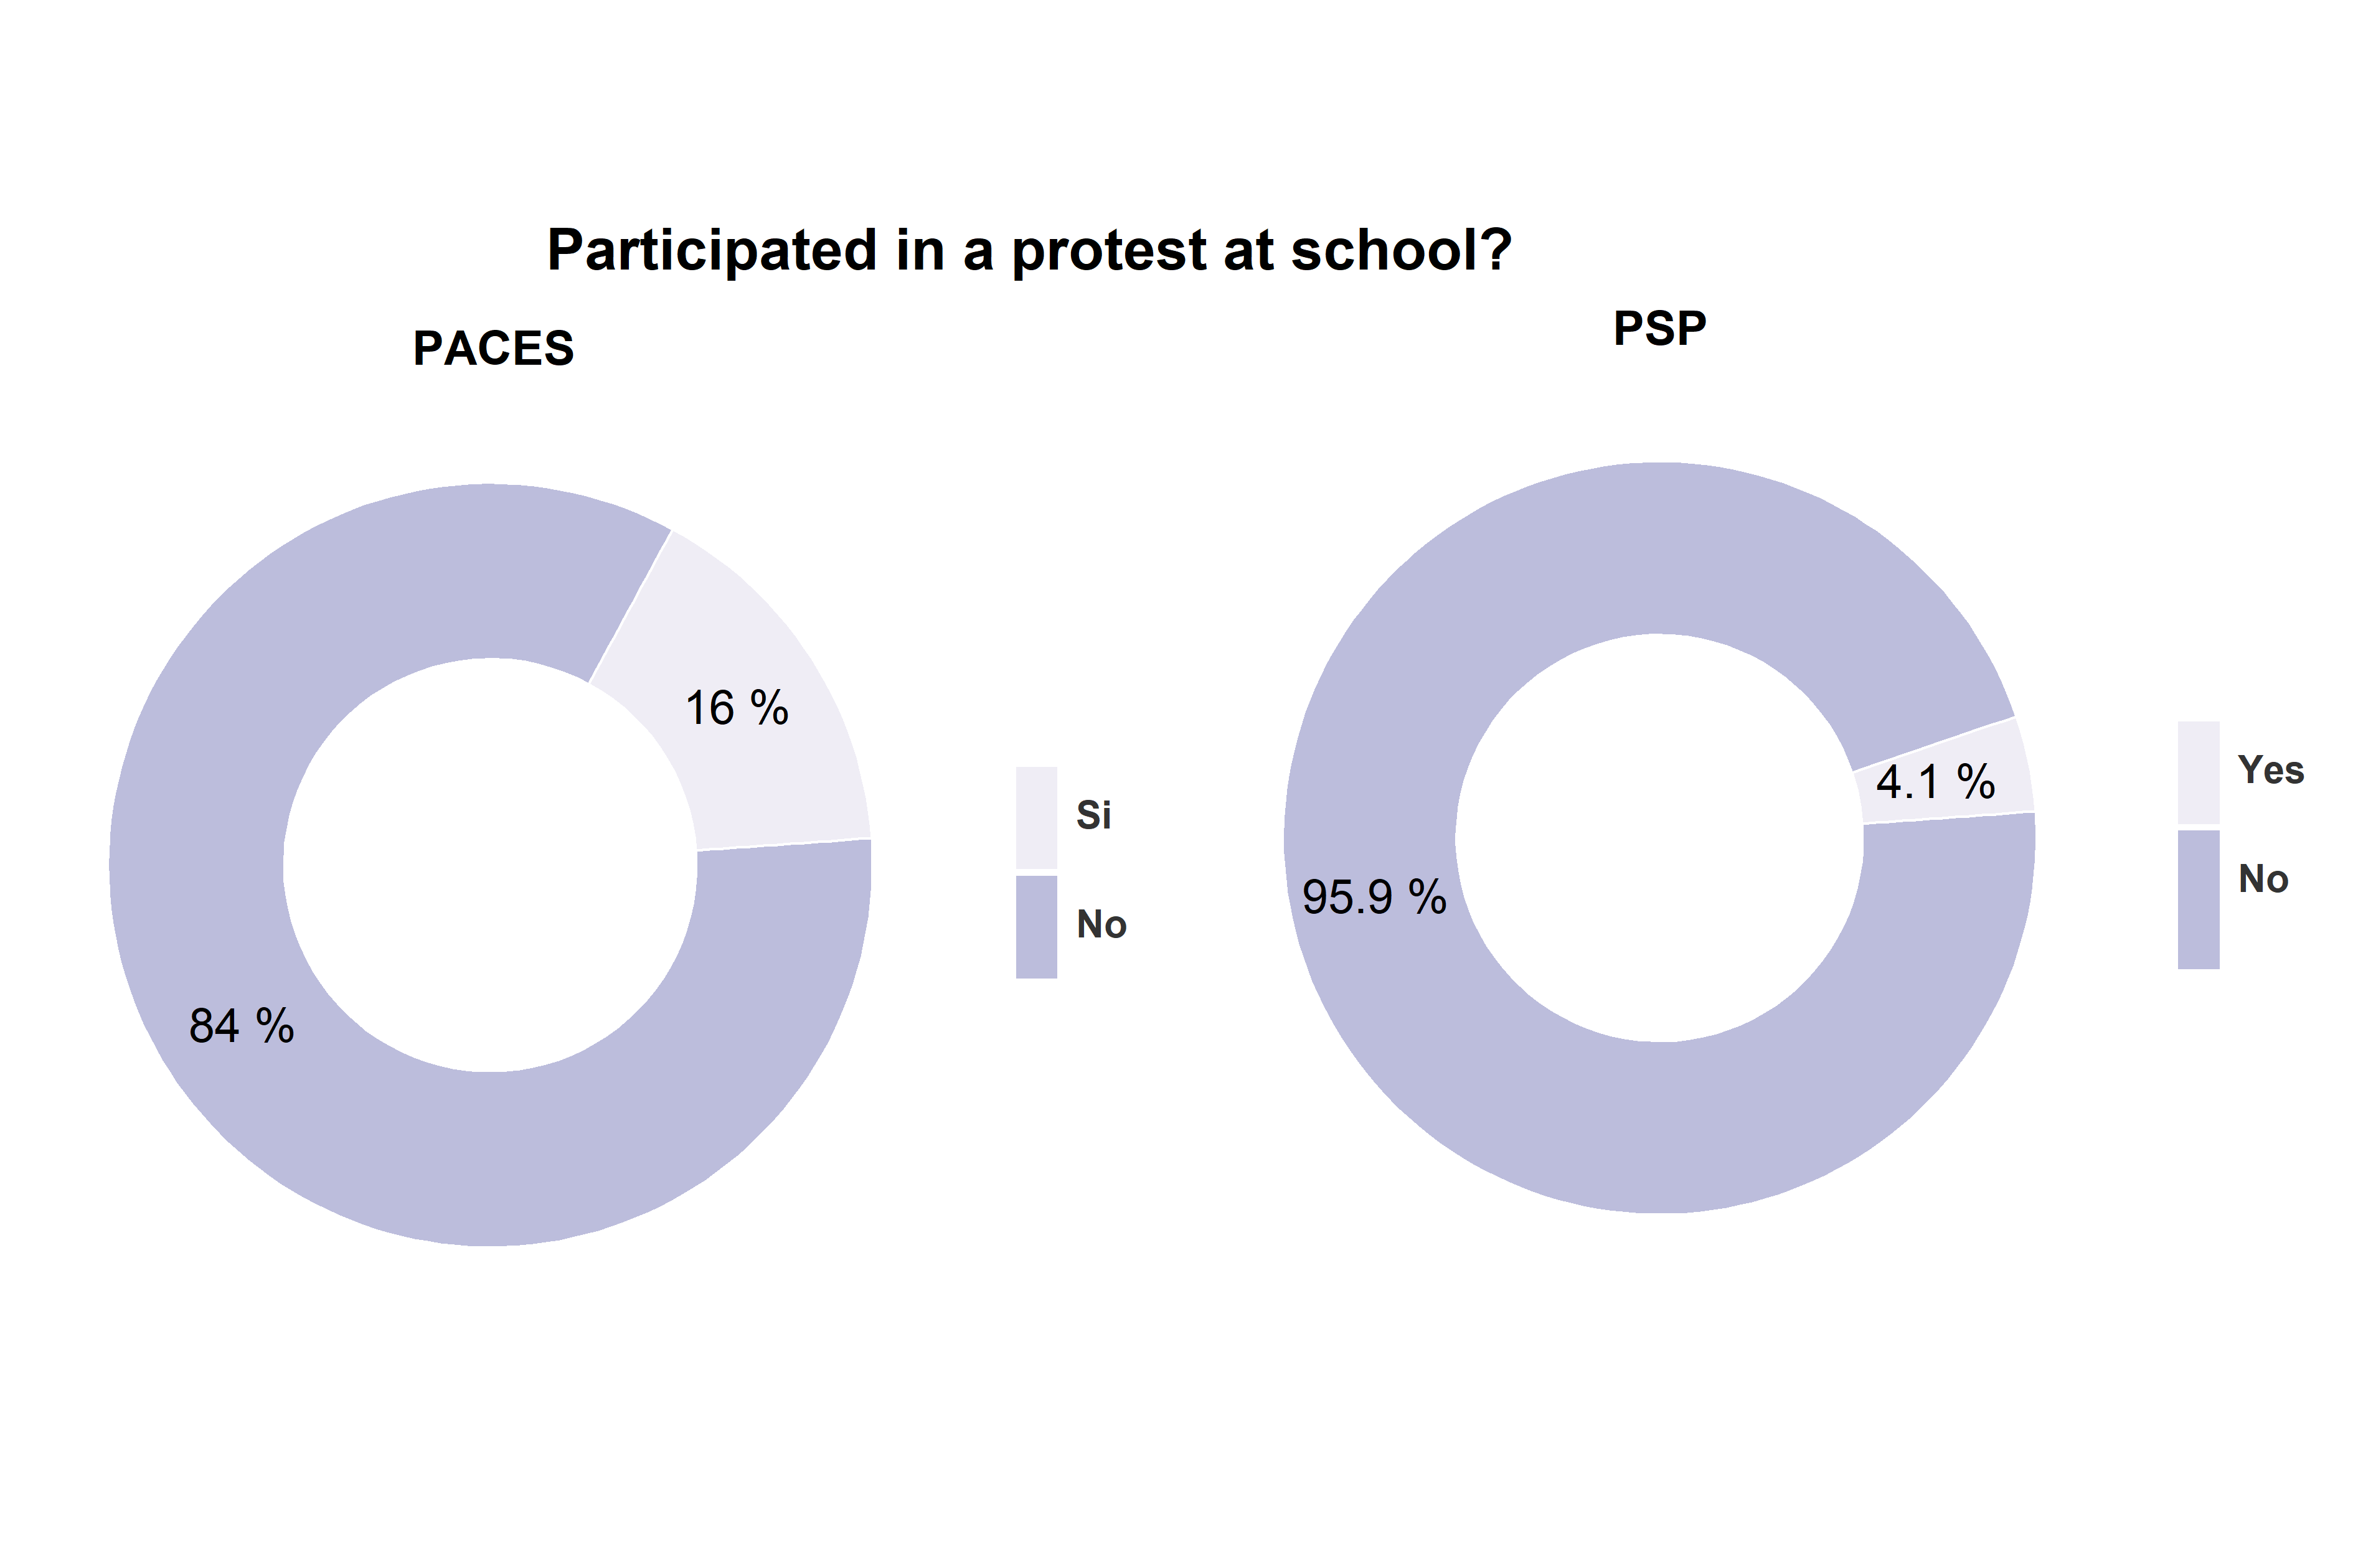
\includegraphics{output/plottr4.png}

\hypertarget{practicas-en-la-escuela}{%
\subsubsection{Practicas en la escuela}\label{practicas-en-la-escuela}}

Se observa una alta participación democratica en la escuela

\begin{verbatim}
## Error in na.omit(.): objeto 'iccs_chsw' no encontrado
\end{verbatim}

\begin{verbatim}
## Error in na.omit(.): objeto 'iccs_chsw' no encontrado
\end{verbatim}

\hypertarget{participaciuxf3n-publica}{%
\subsubsection{Participación publica}\label{participaciuxf3n-publica}}

\textbf{Youth participation}

\textbf{Signed a petition?}

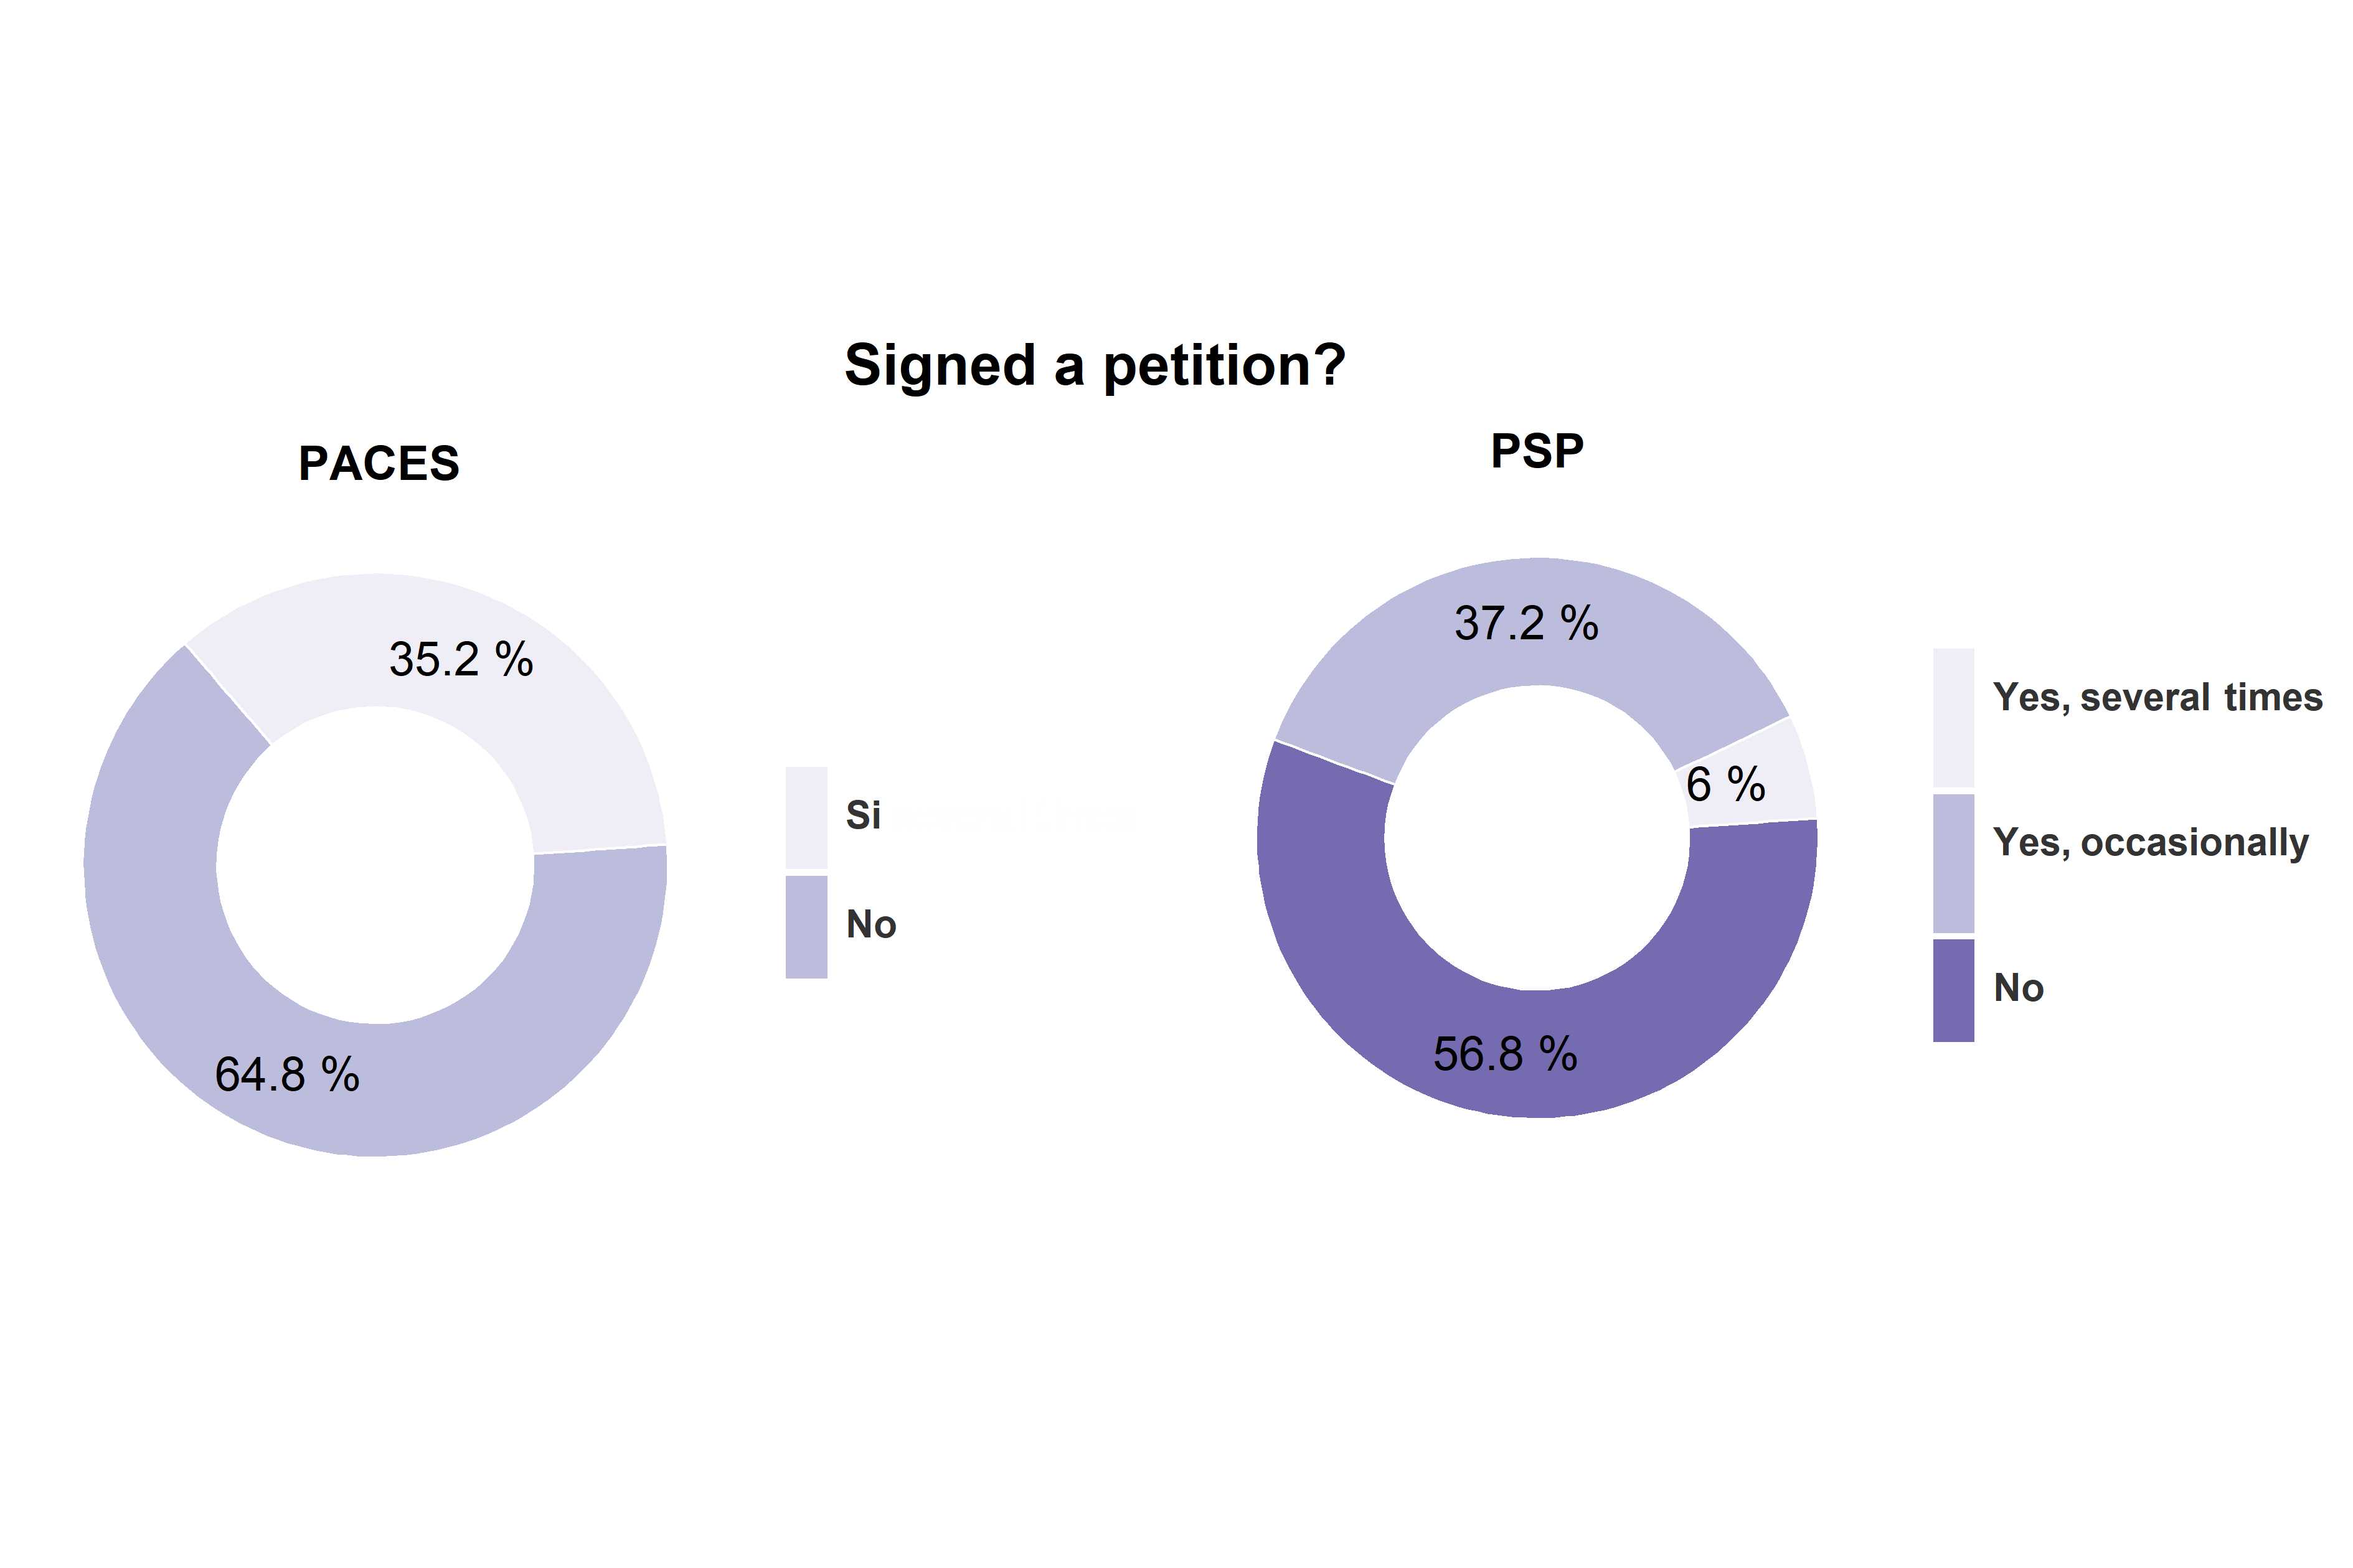
\includegraphics{output/plotyp1.png}

\textbf{Worked voluntarily for a good cause?}

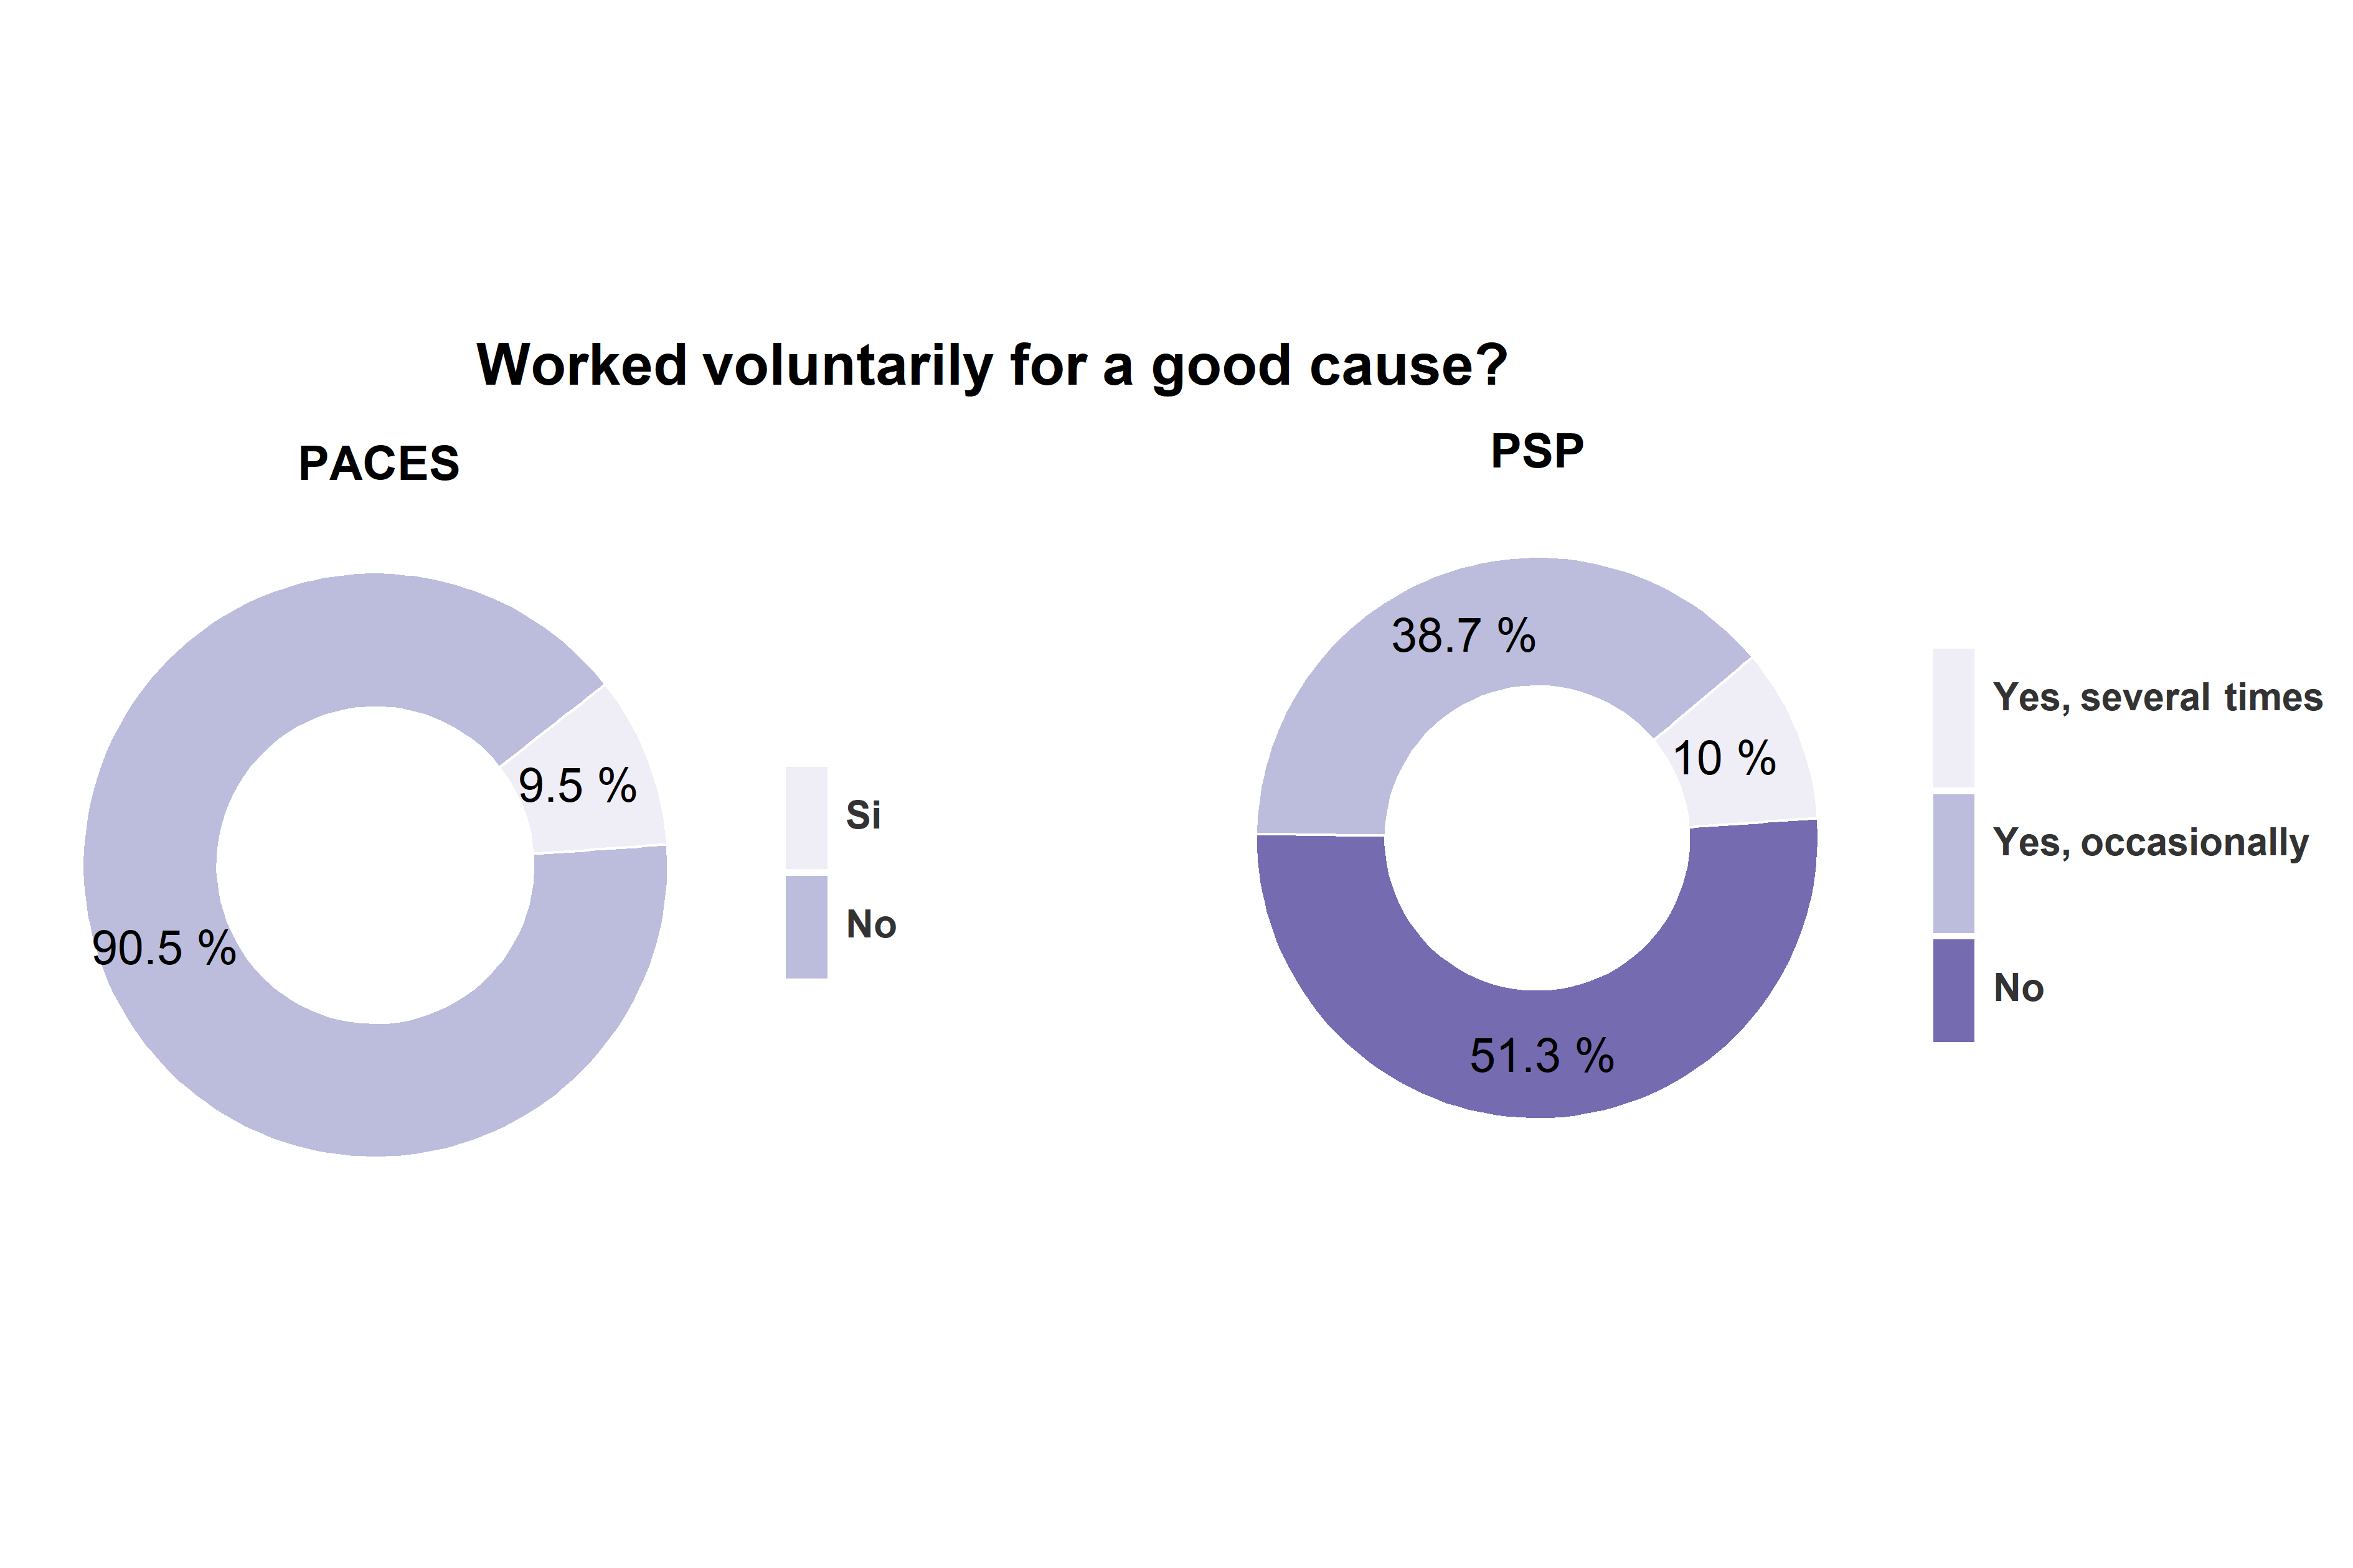
\includegraphics{output/plotyp2.png}

\textbf{Taken part in a legal demonstration or strike?}

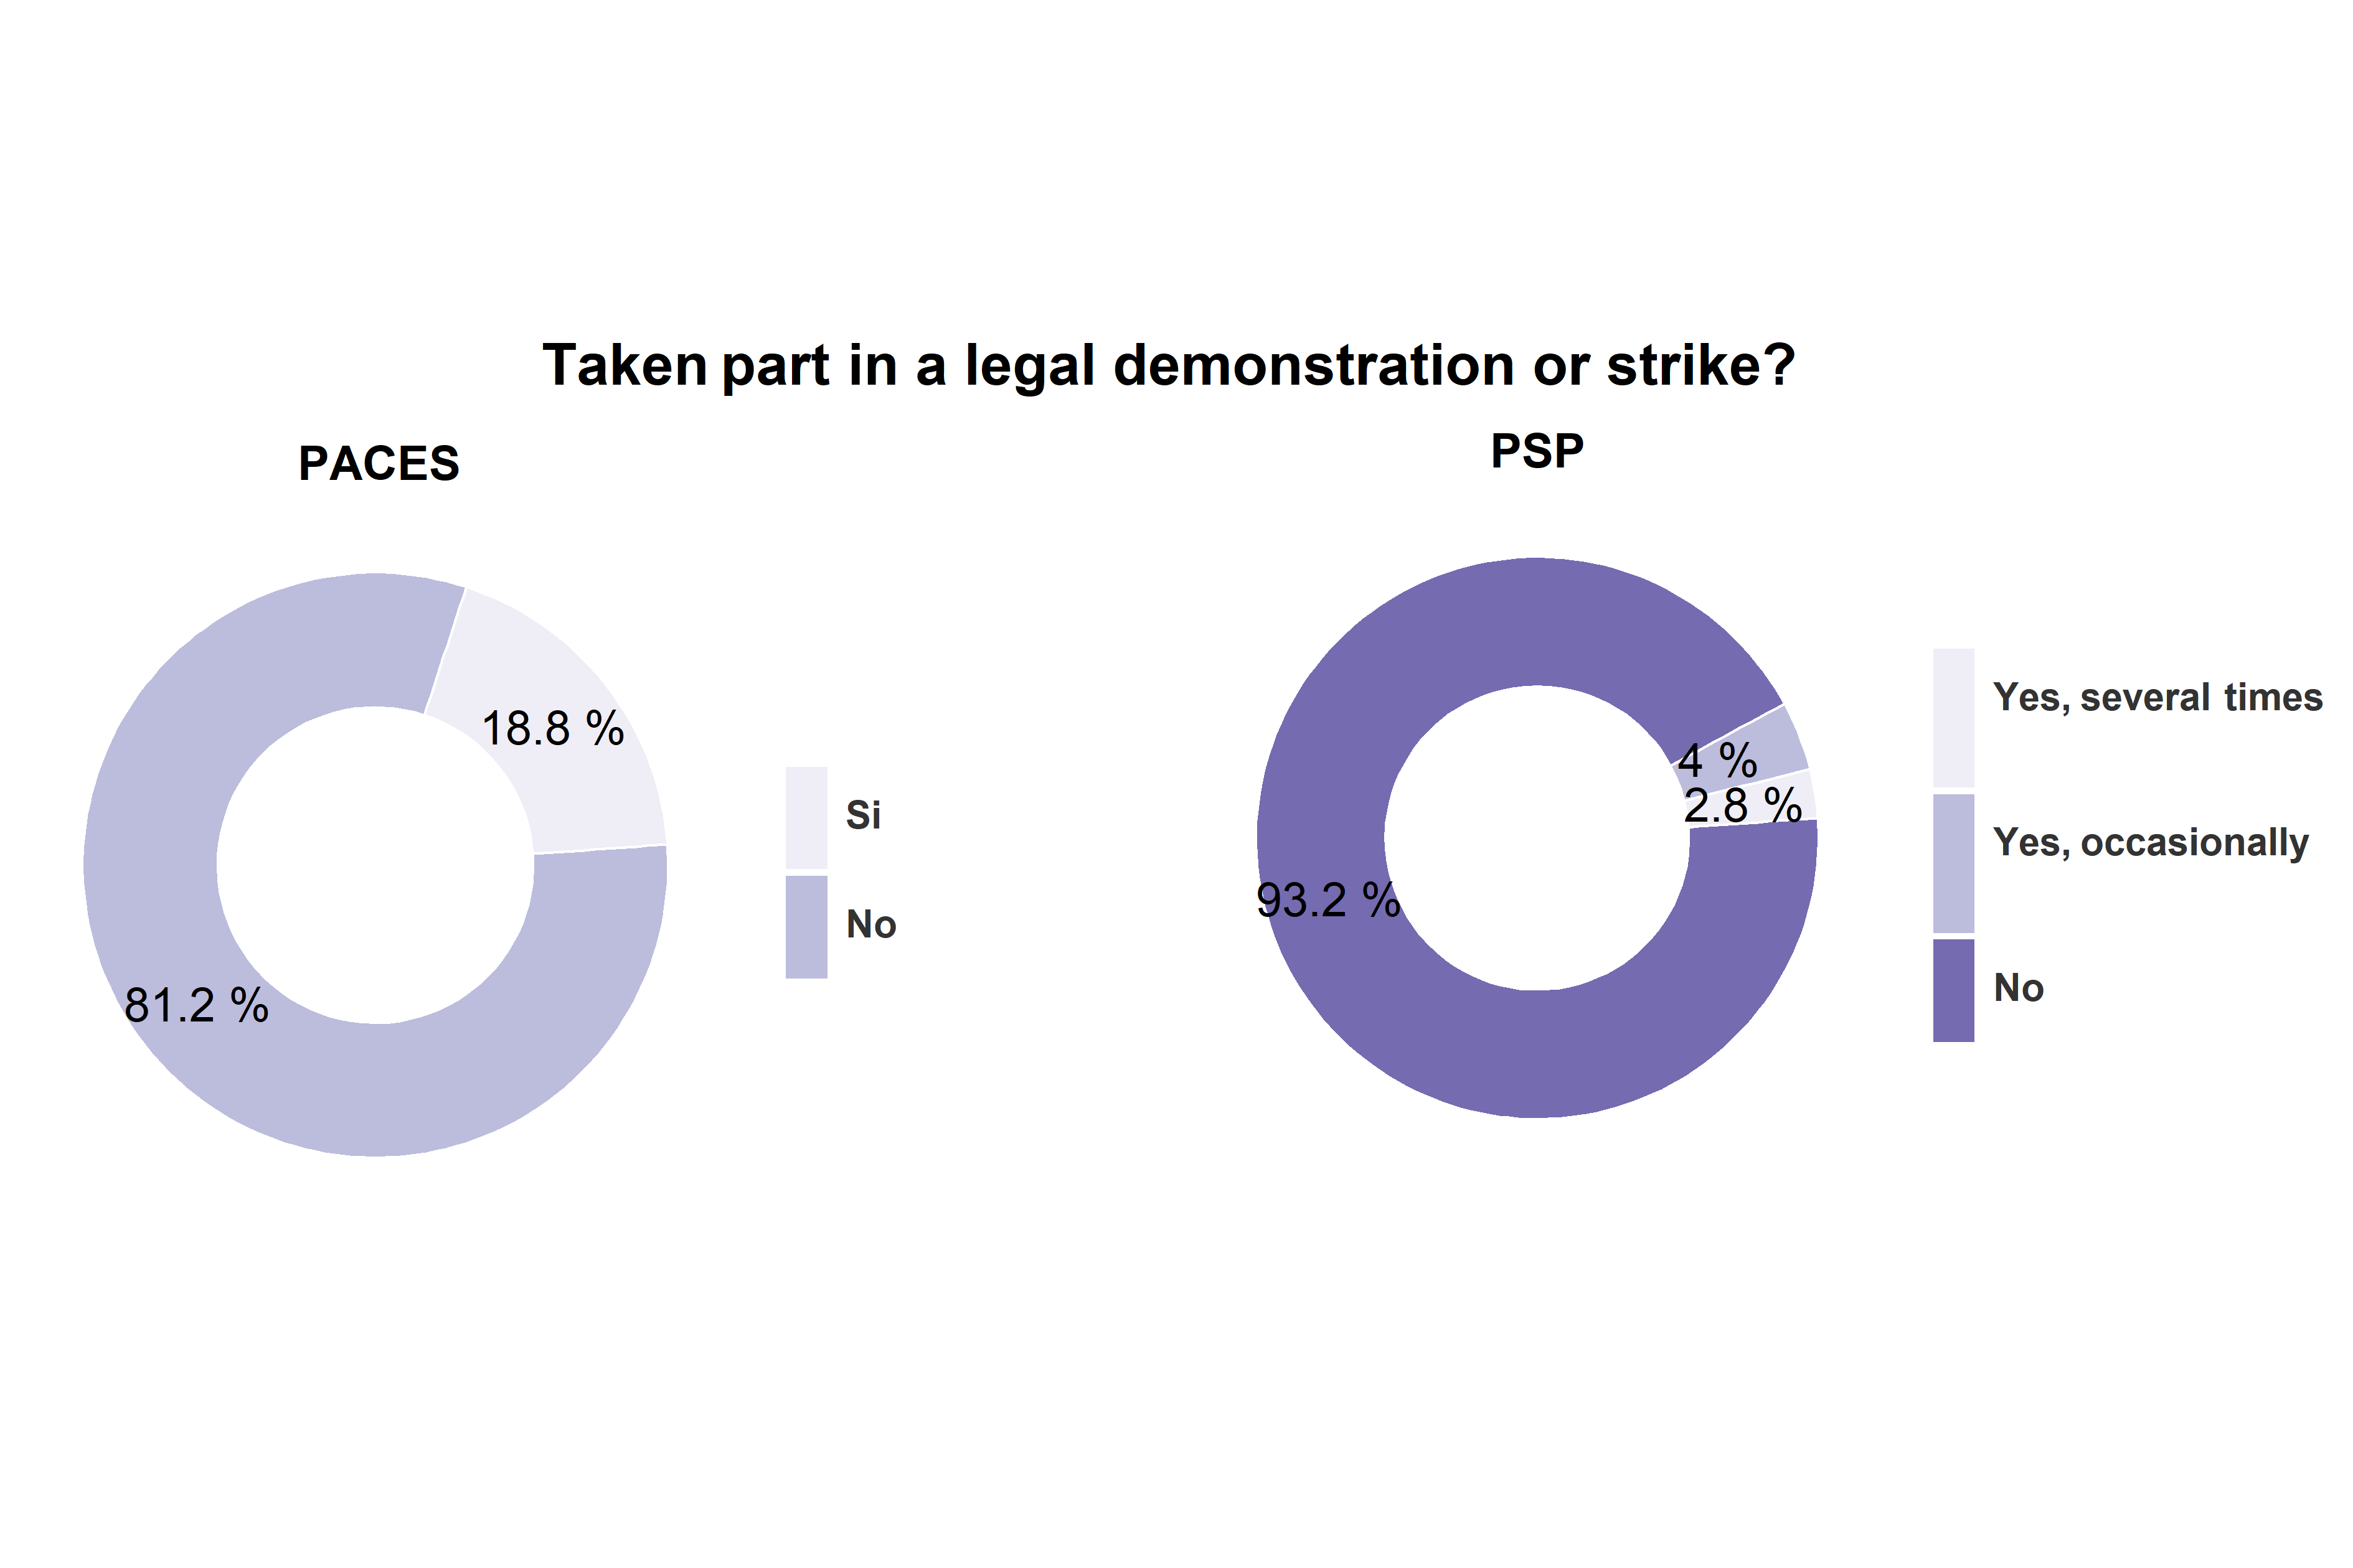
\includegraphics{output/plotyp3.png}

\textbf{Occupation}

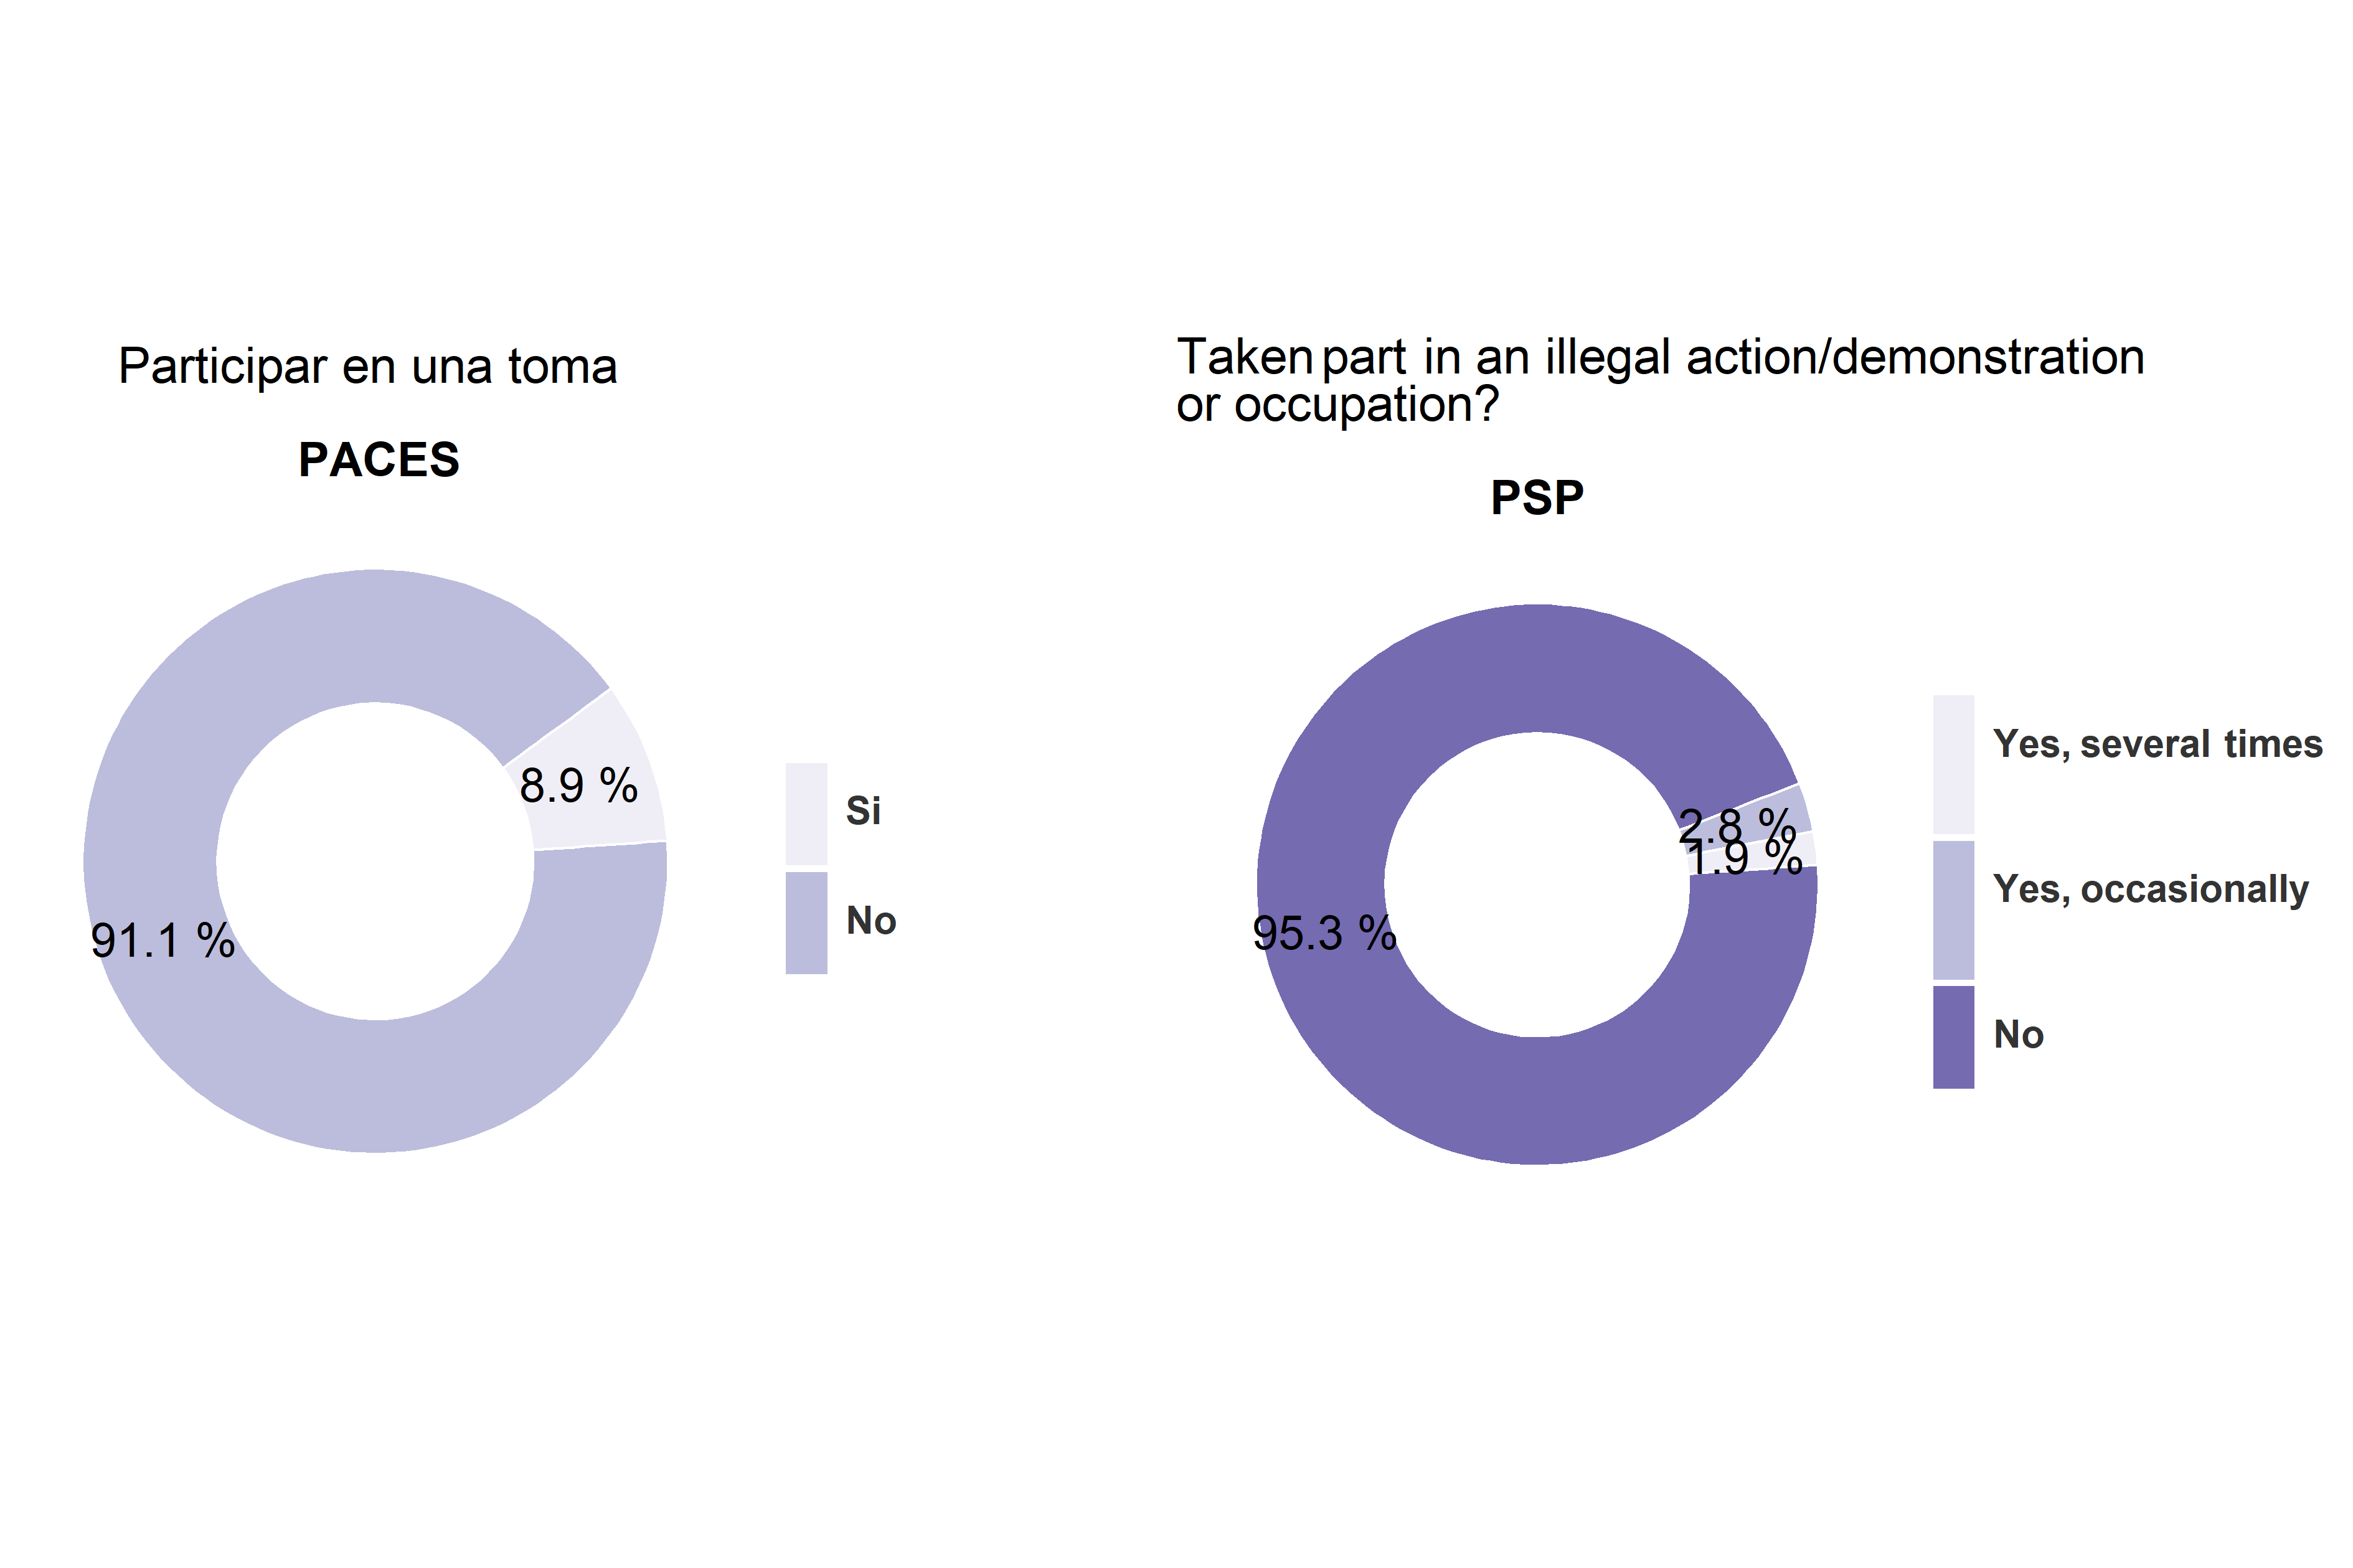
\includegraphics{output/plotyp4.png}

\textbf{Ilegal strike}

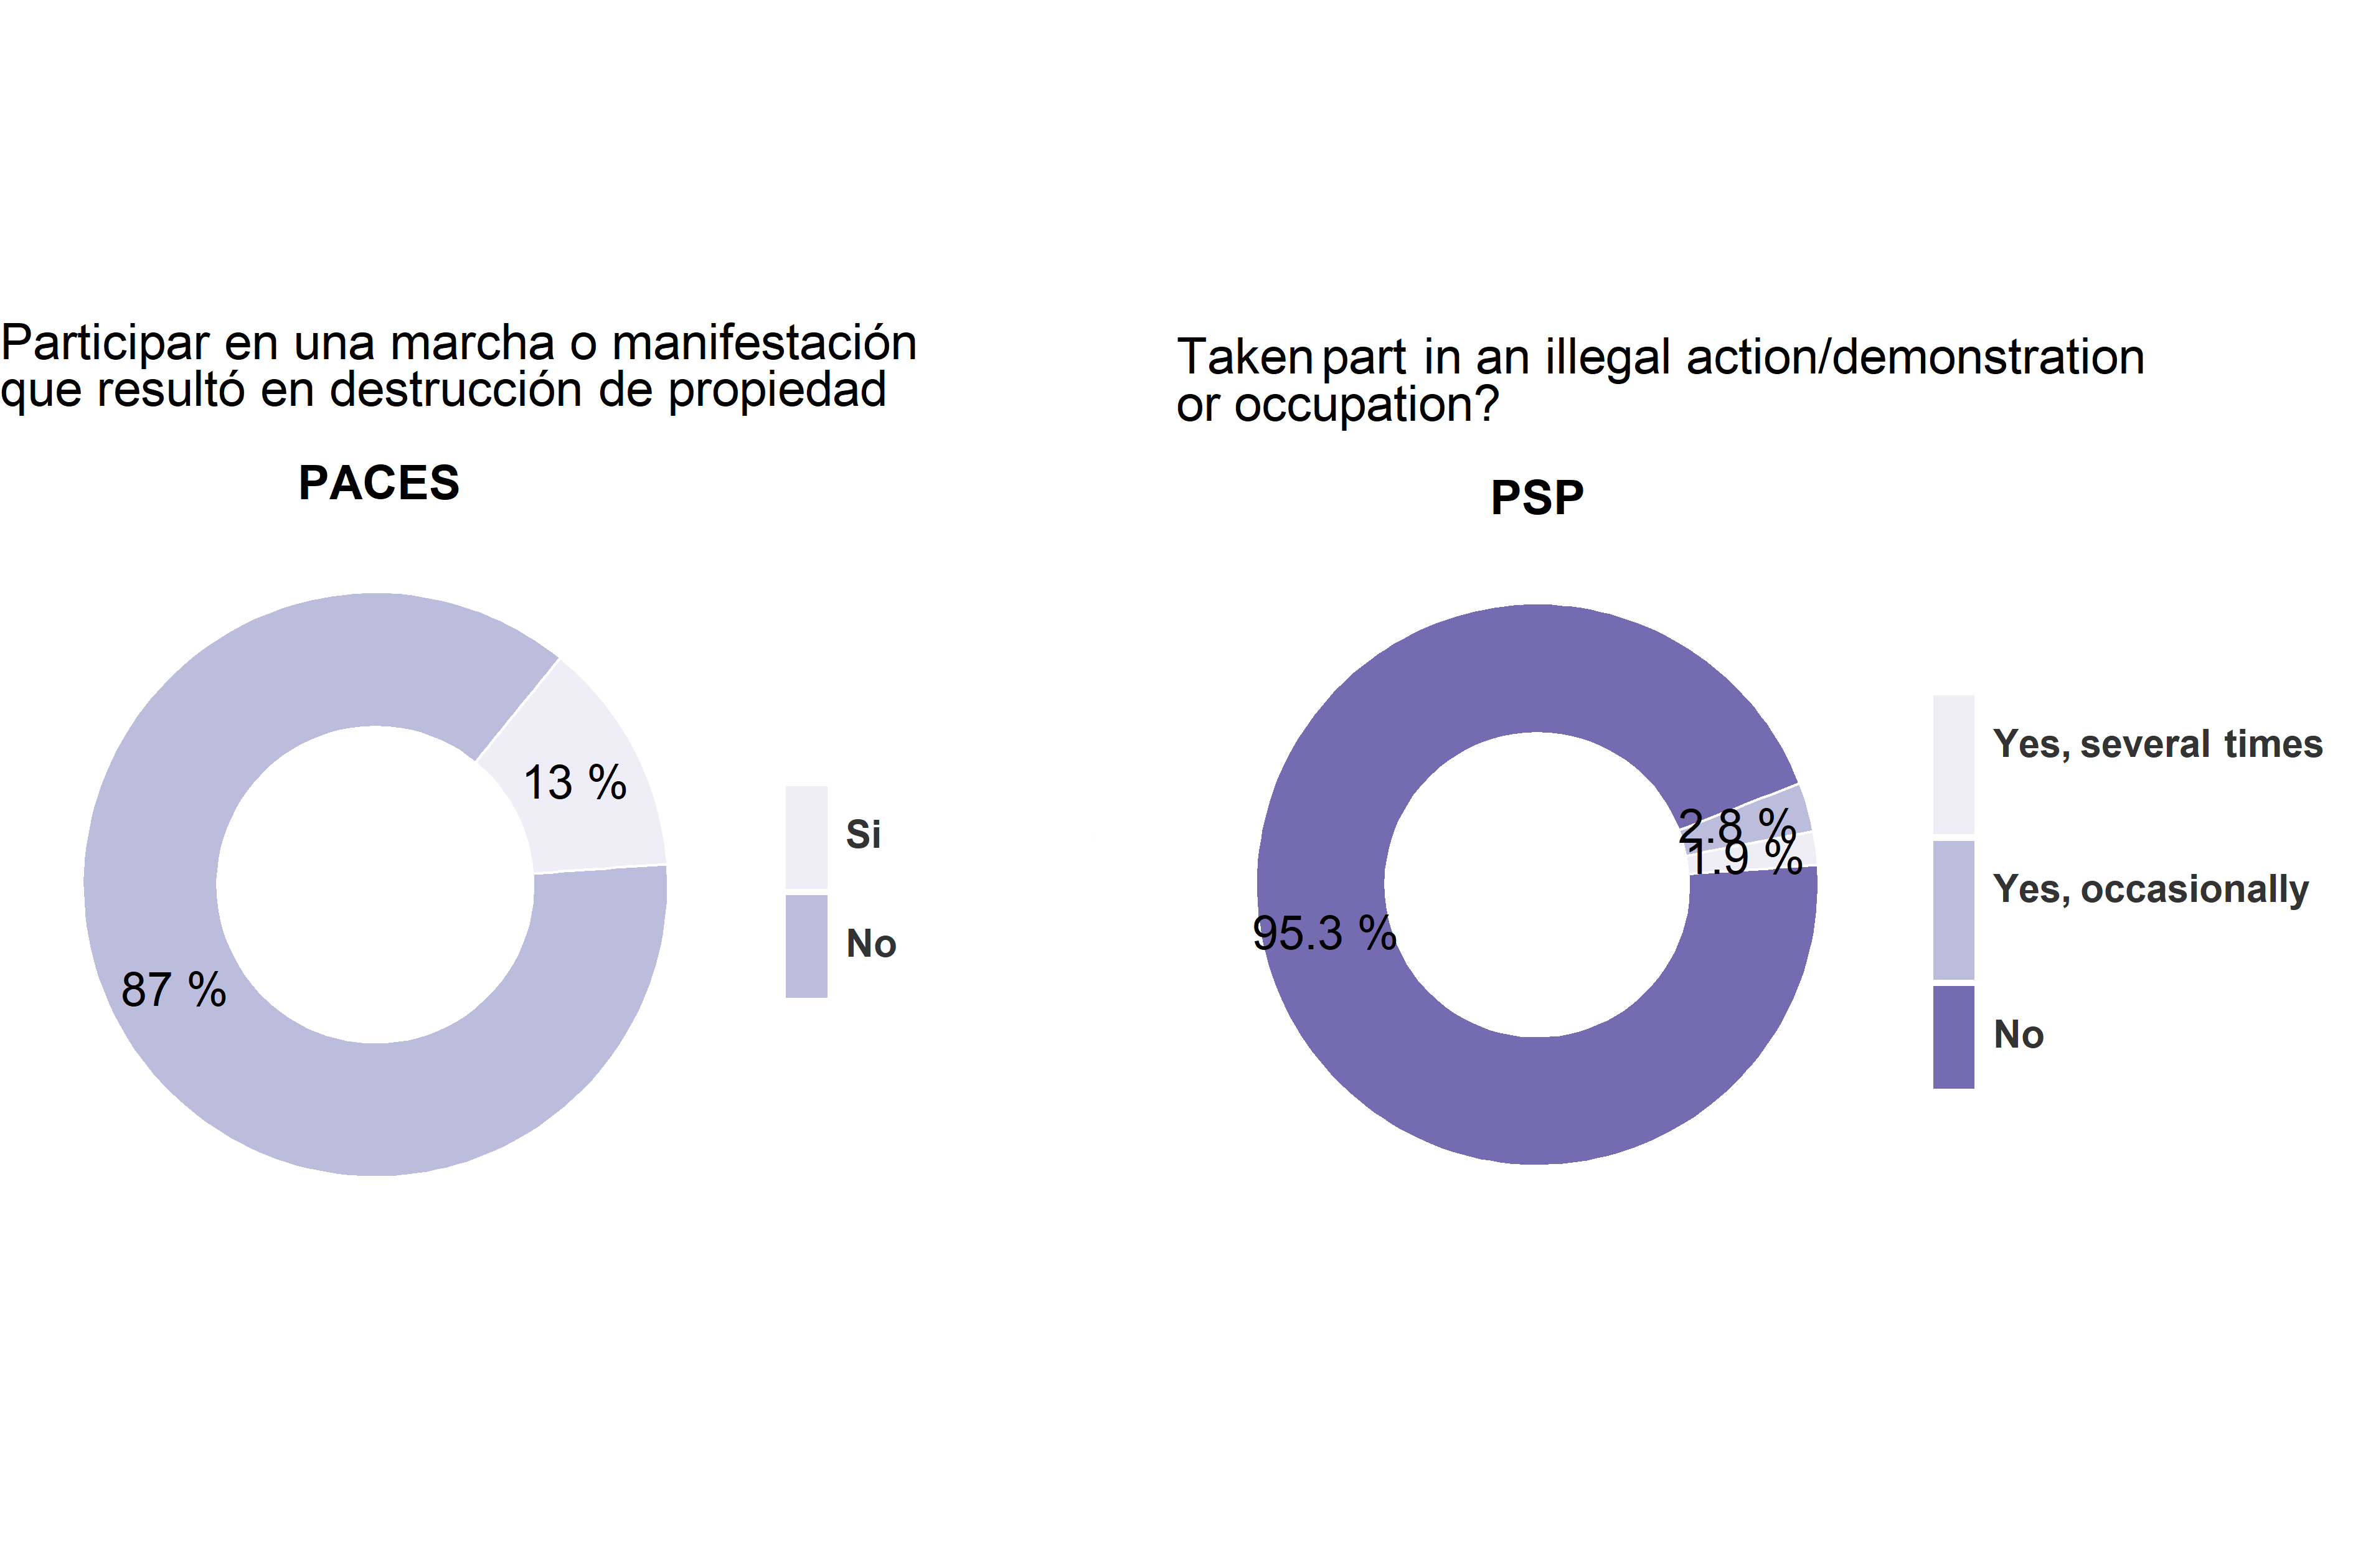
\includegraphics{output/plotyp5.png}

\hypertarget{socializaciuxf3n-politica-y-discuciuxf3n-ciudadana}{%
\subsubsection{Socialización politica y discución ciudadana}\label{socializaciuxf3n-politica-y-discuciuxf3n-ciudadana}}

\textbf{Environmental issues}

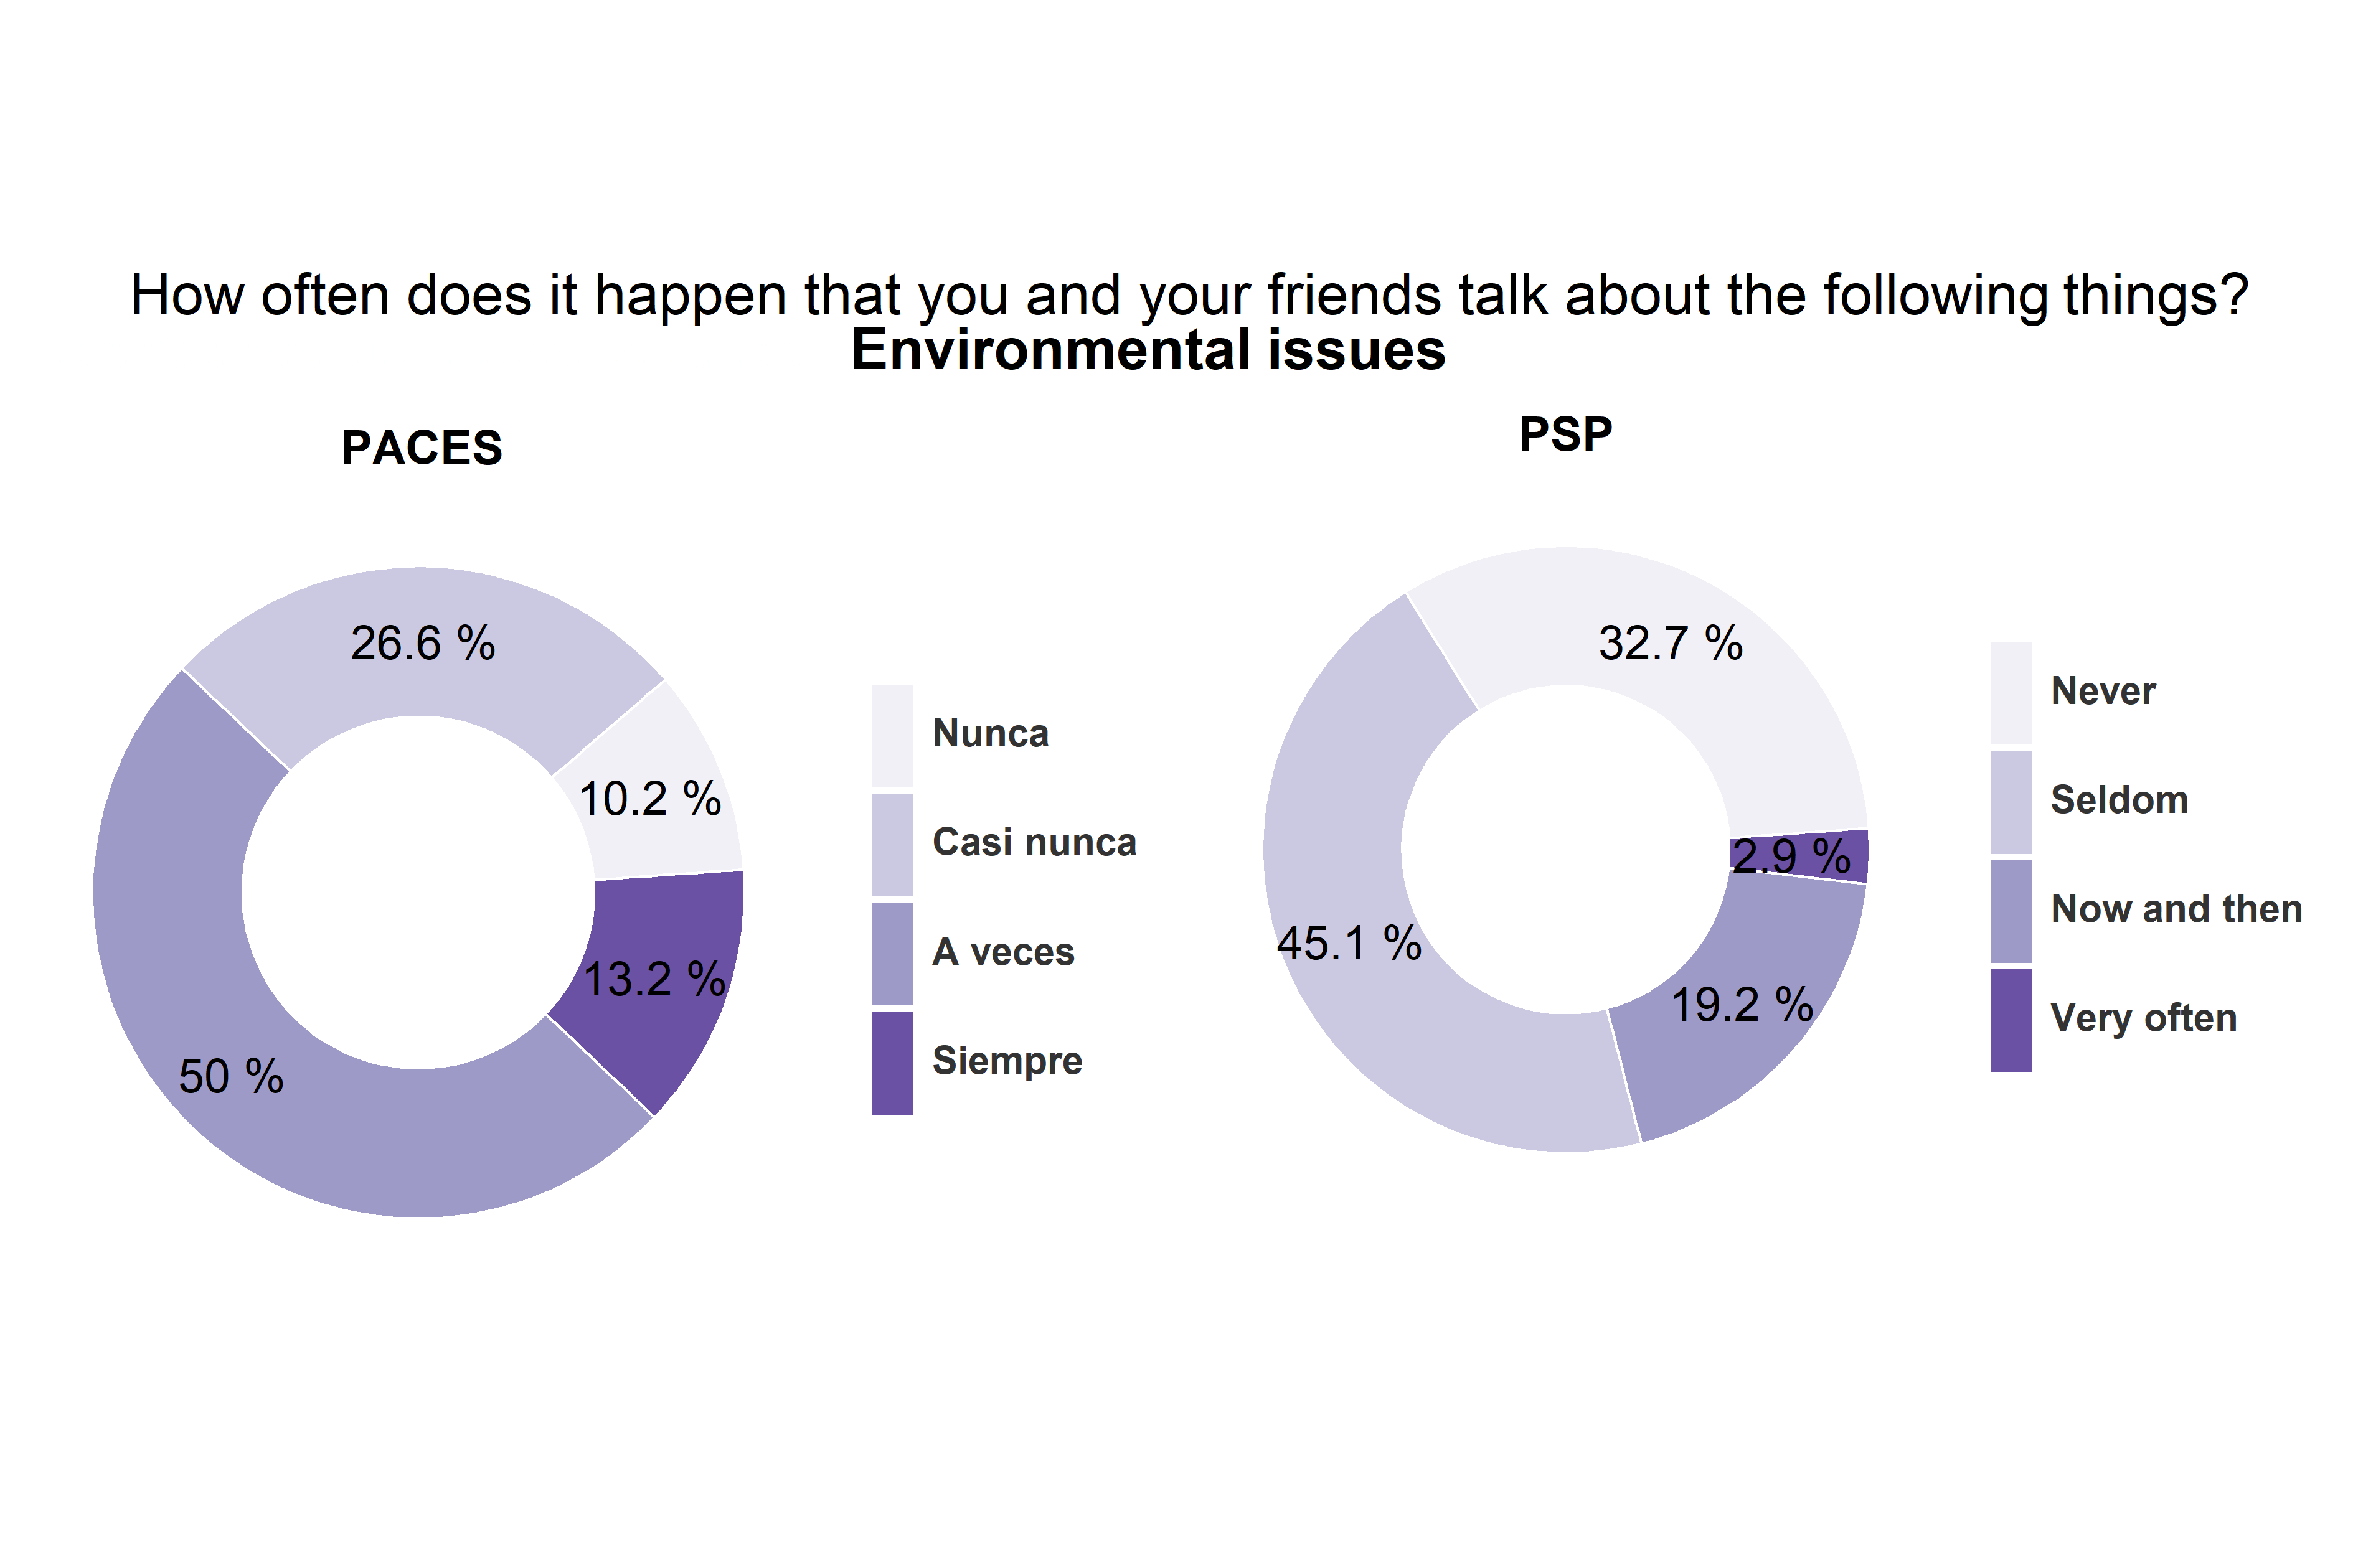
\includegraphics{output/plotdiscper1.png}

\textbf{Facebook and contacts with others on the Internet}

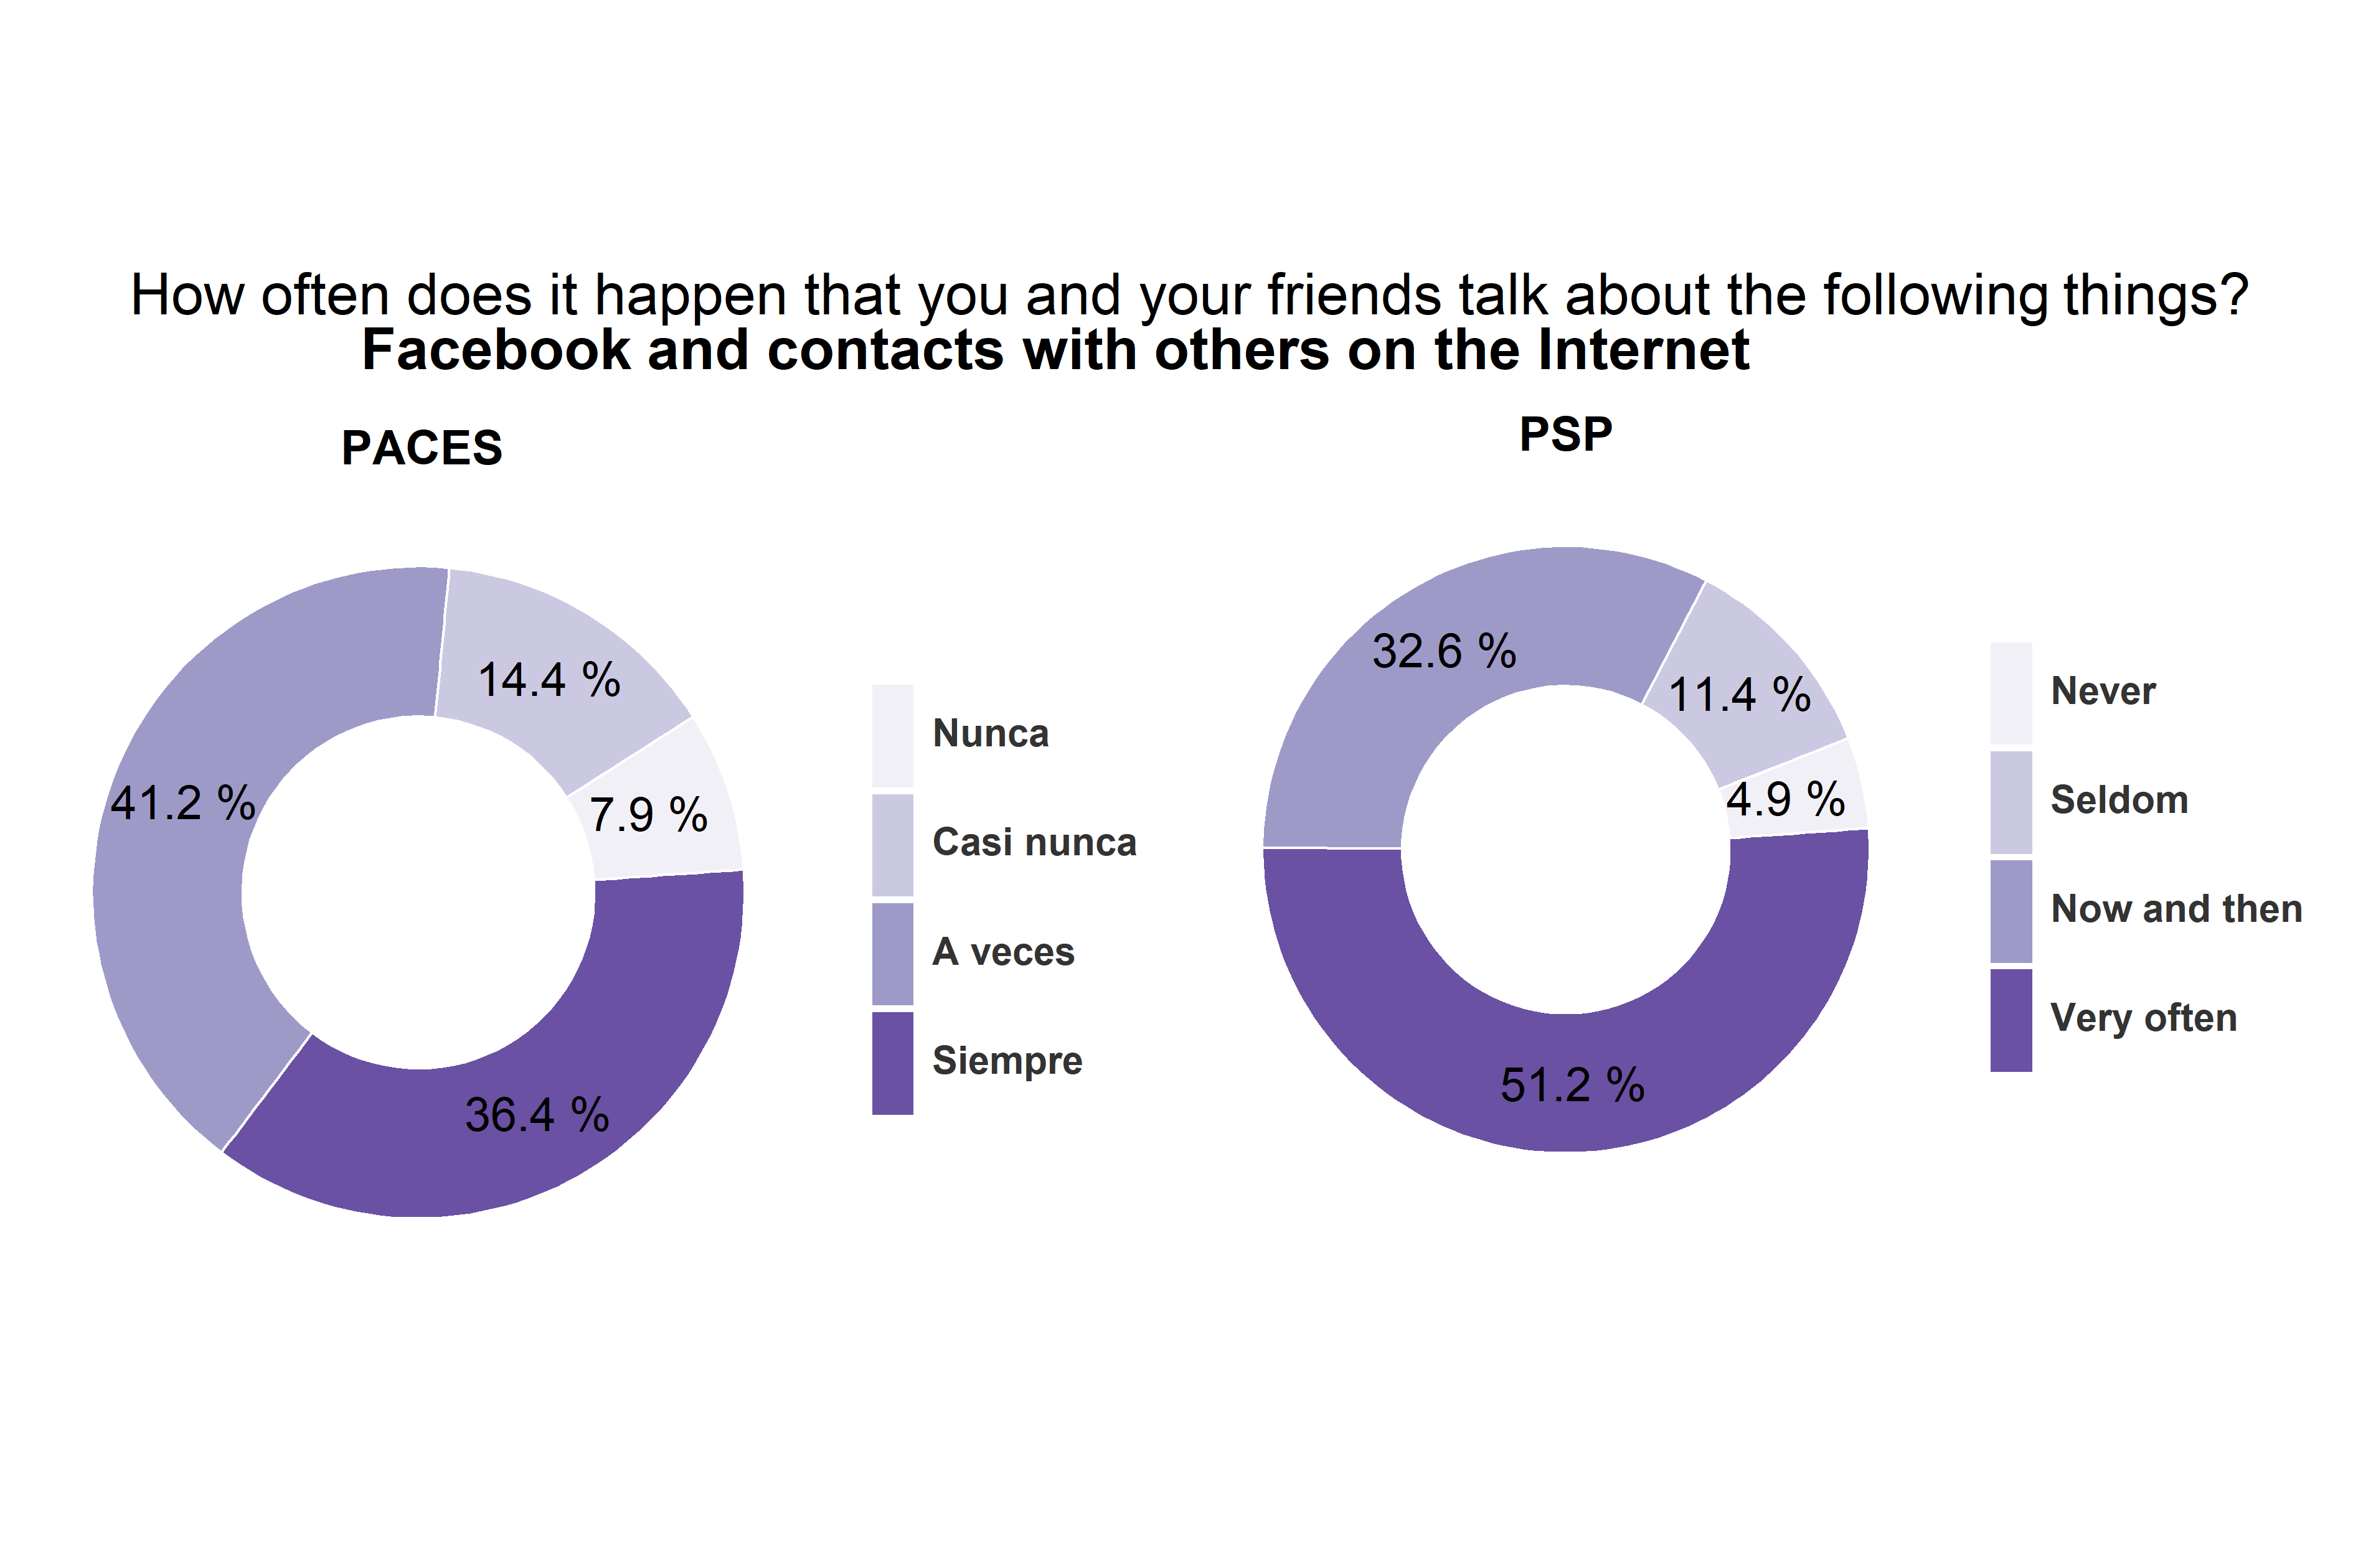
\includegraphics{output/plotdiscper2.png}

\textbf{Politics or societal issues}

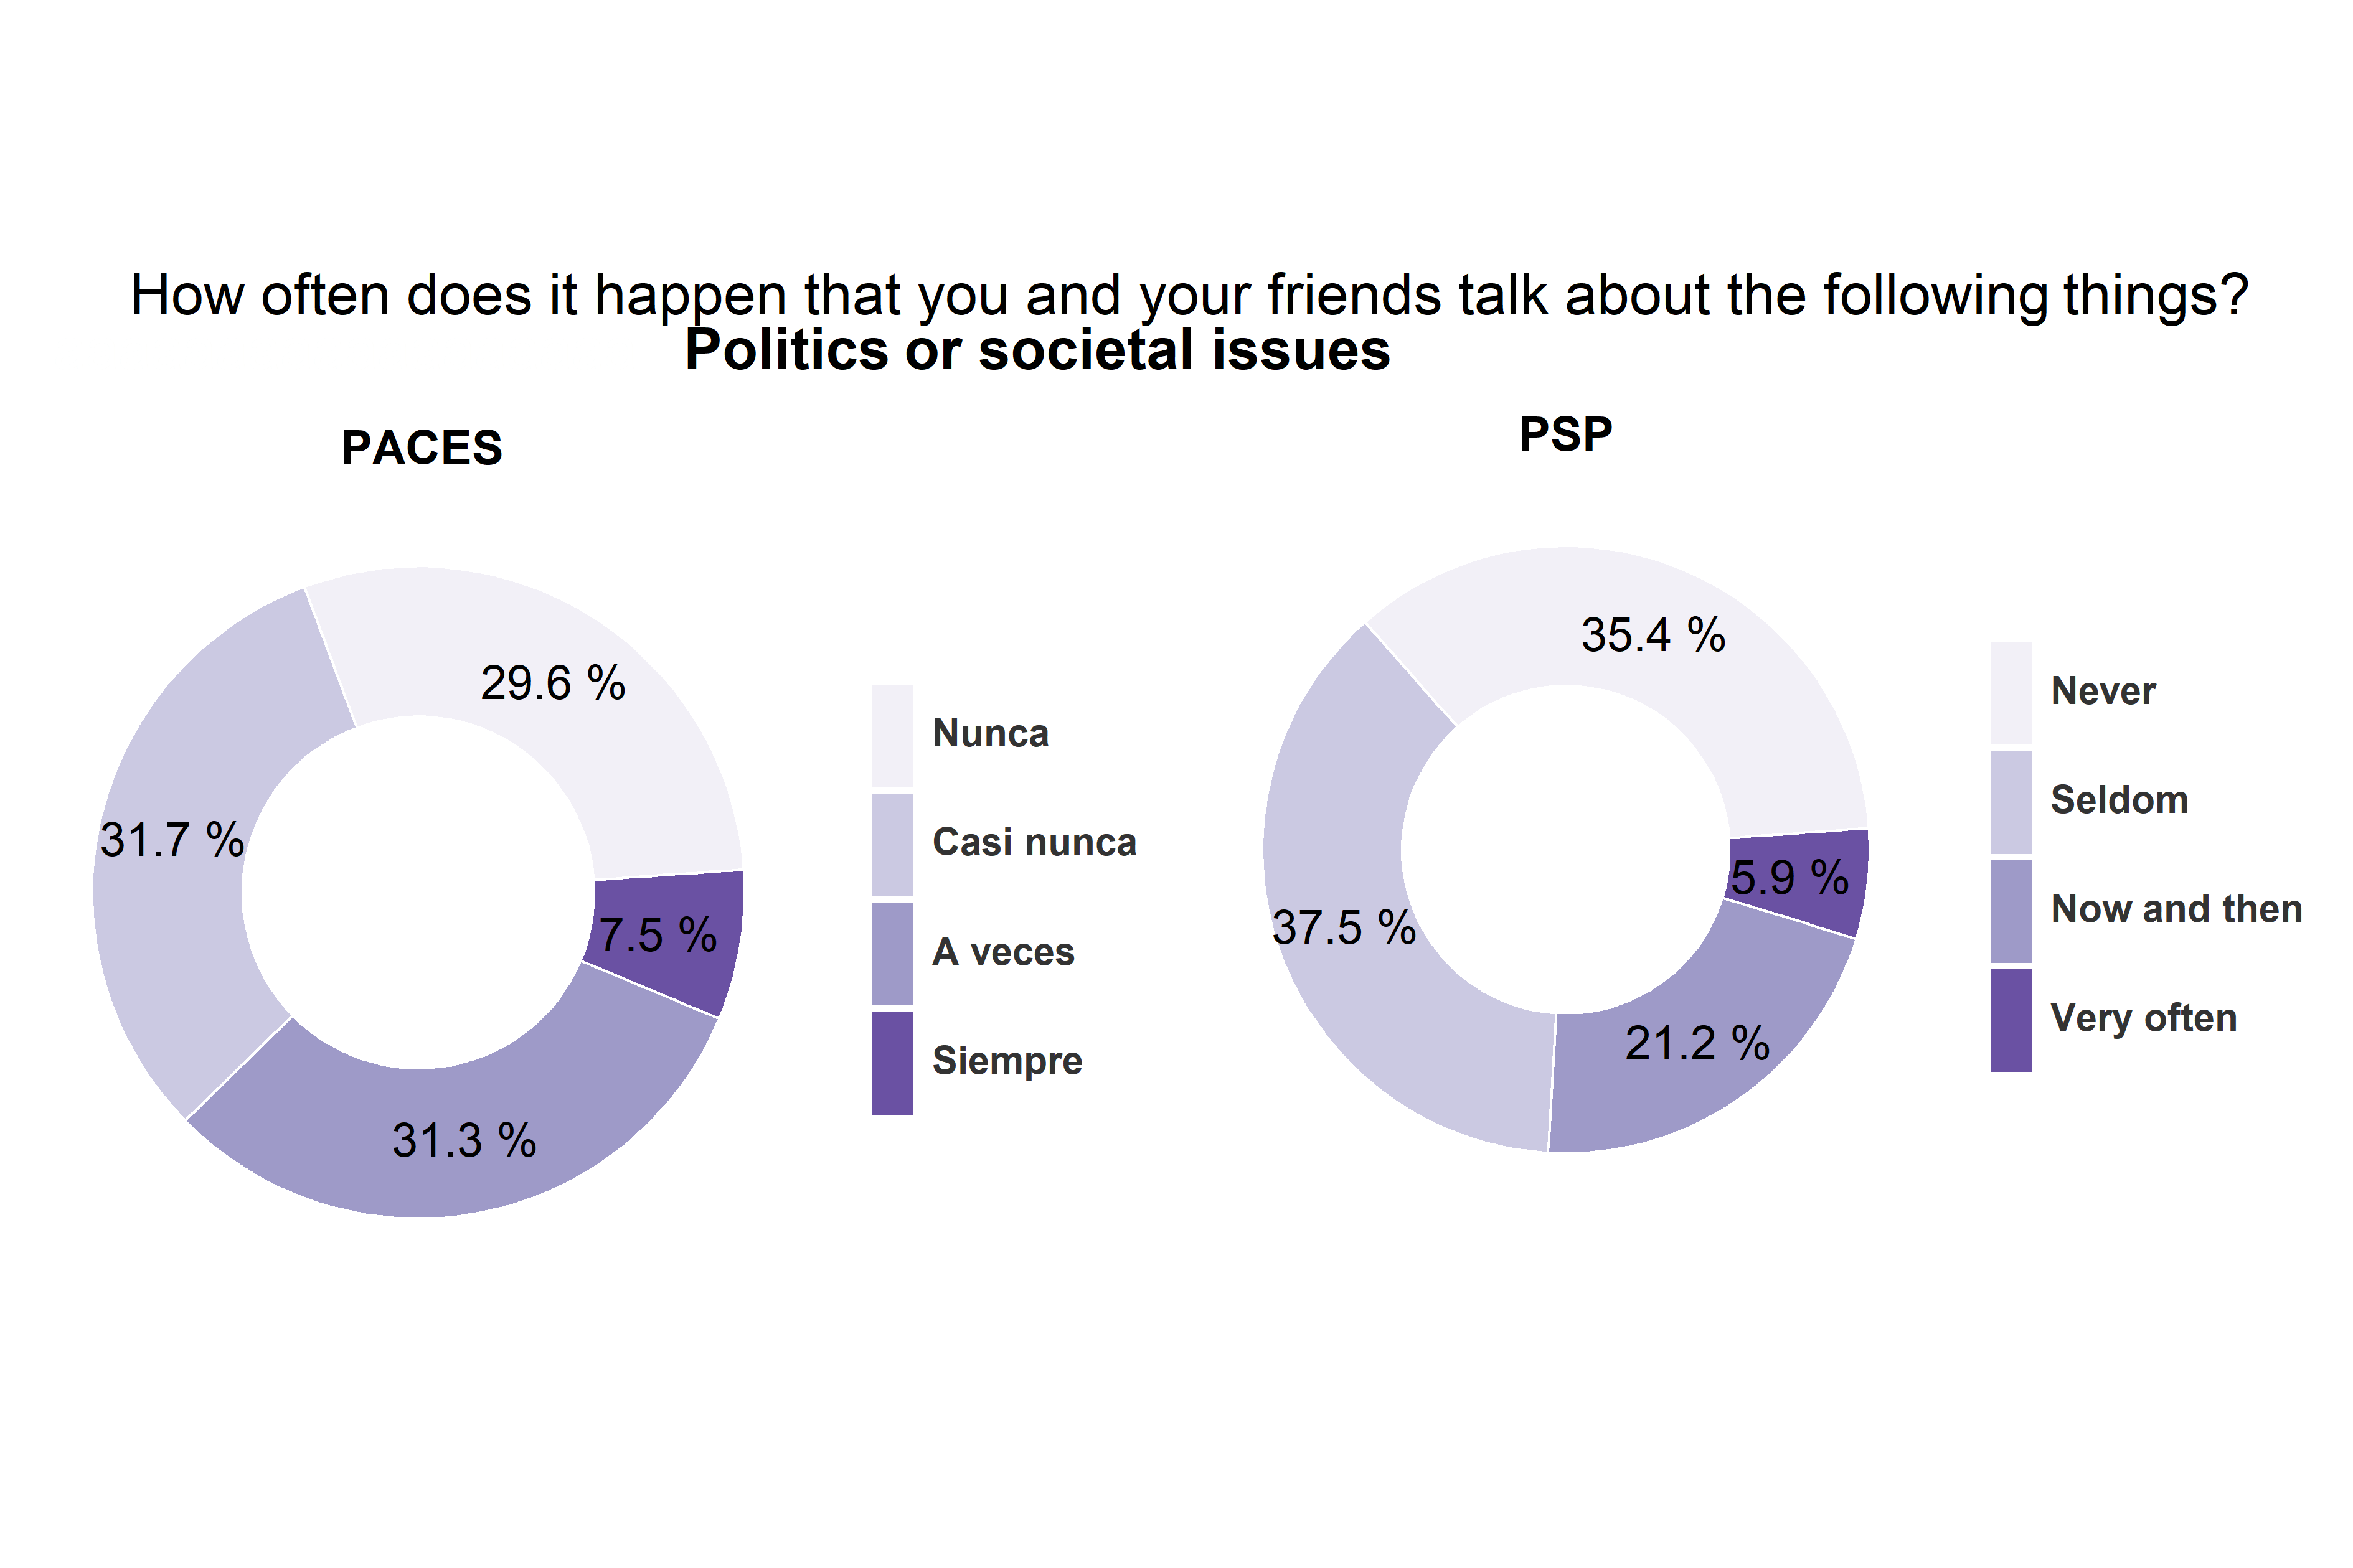
\includegraphics{output/plotdiscper3.png}

\textbf{What you have heard on the news about what is going on in ´country´ and around the world}

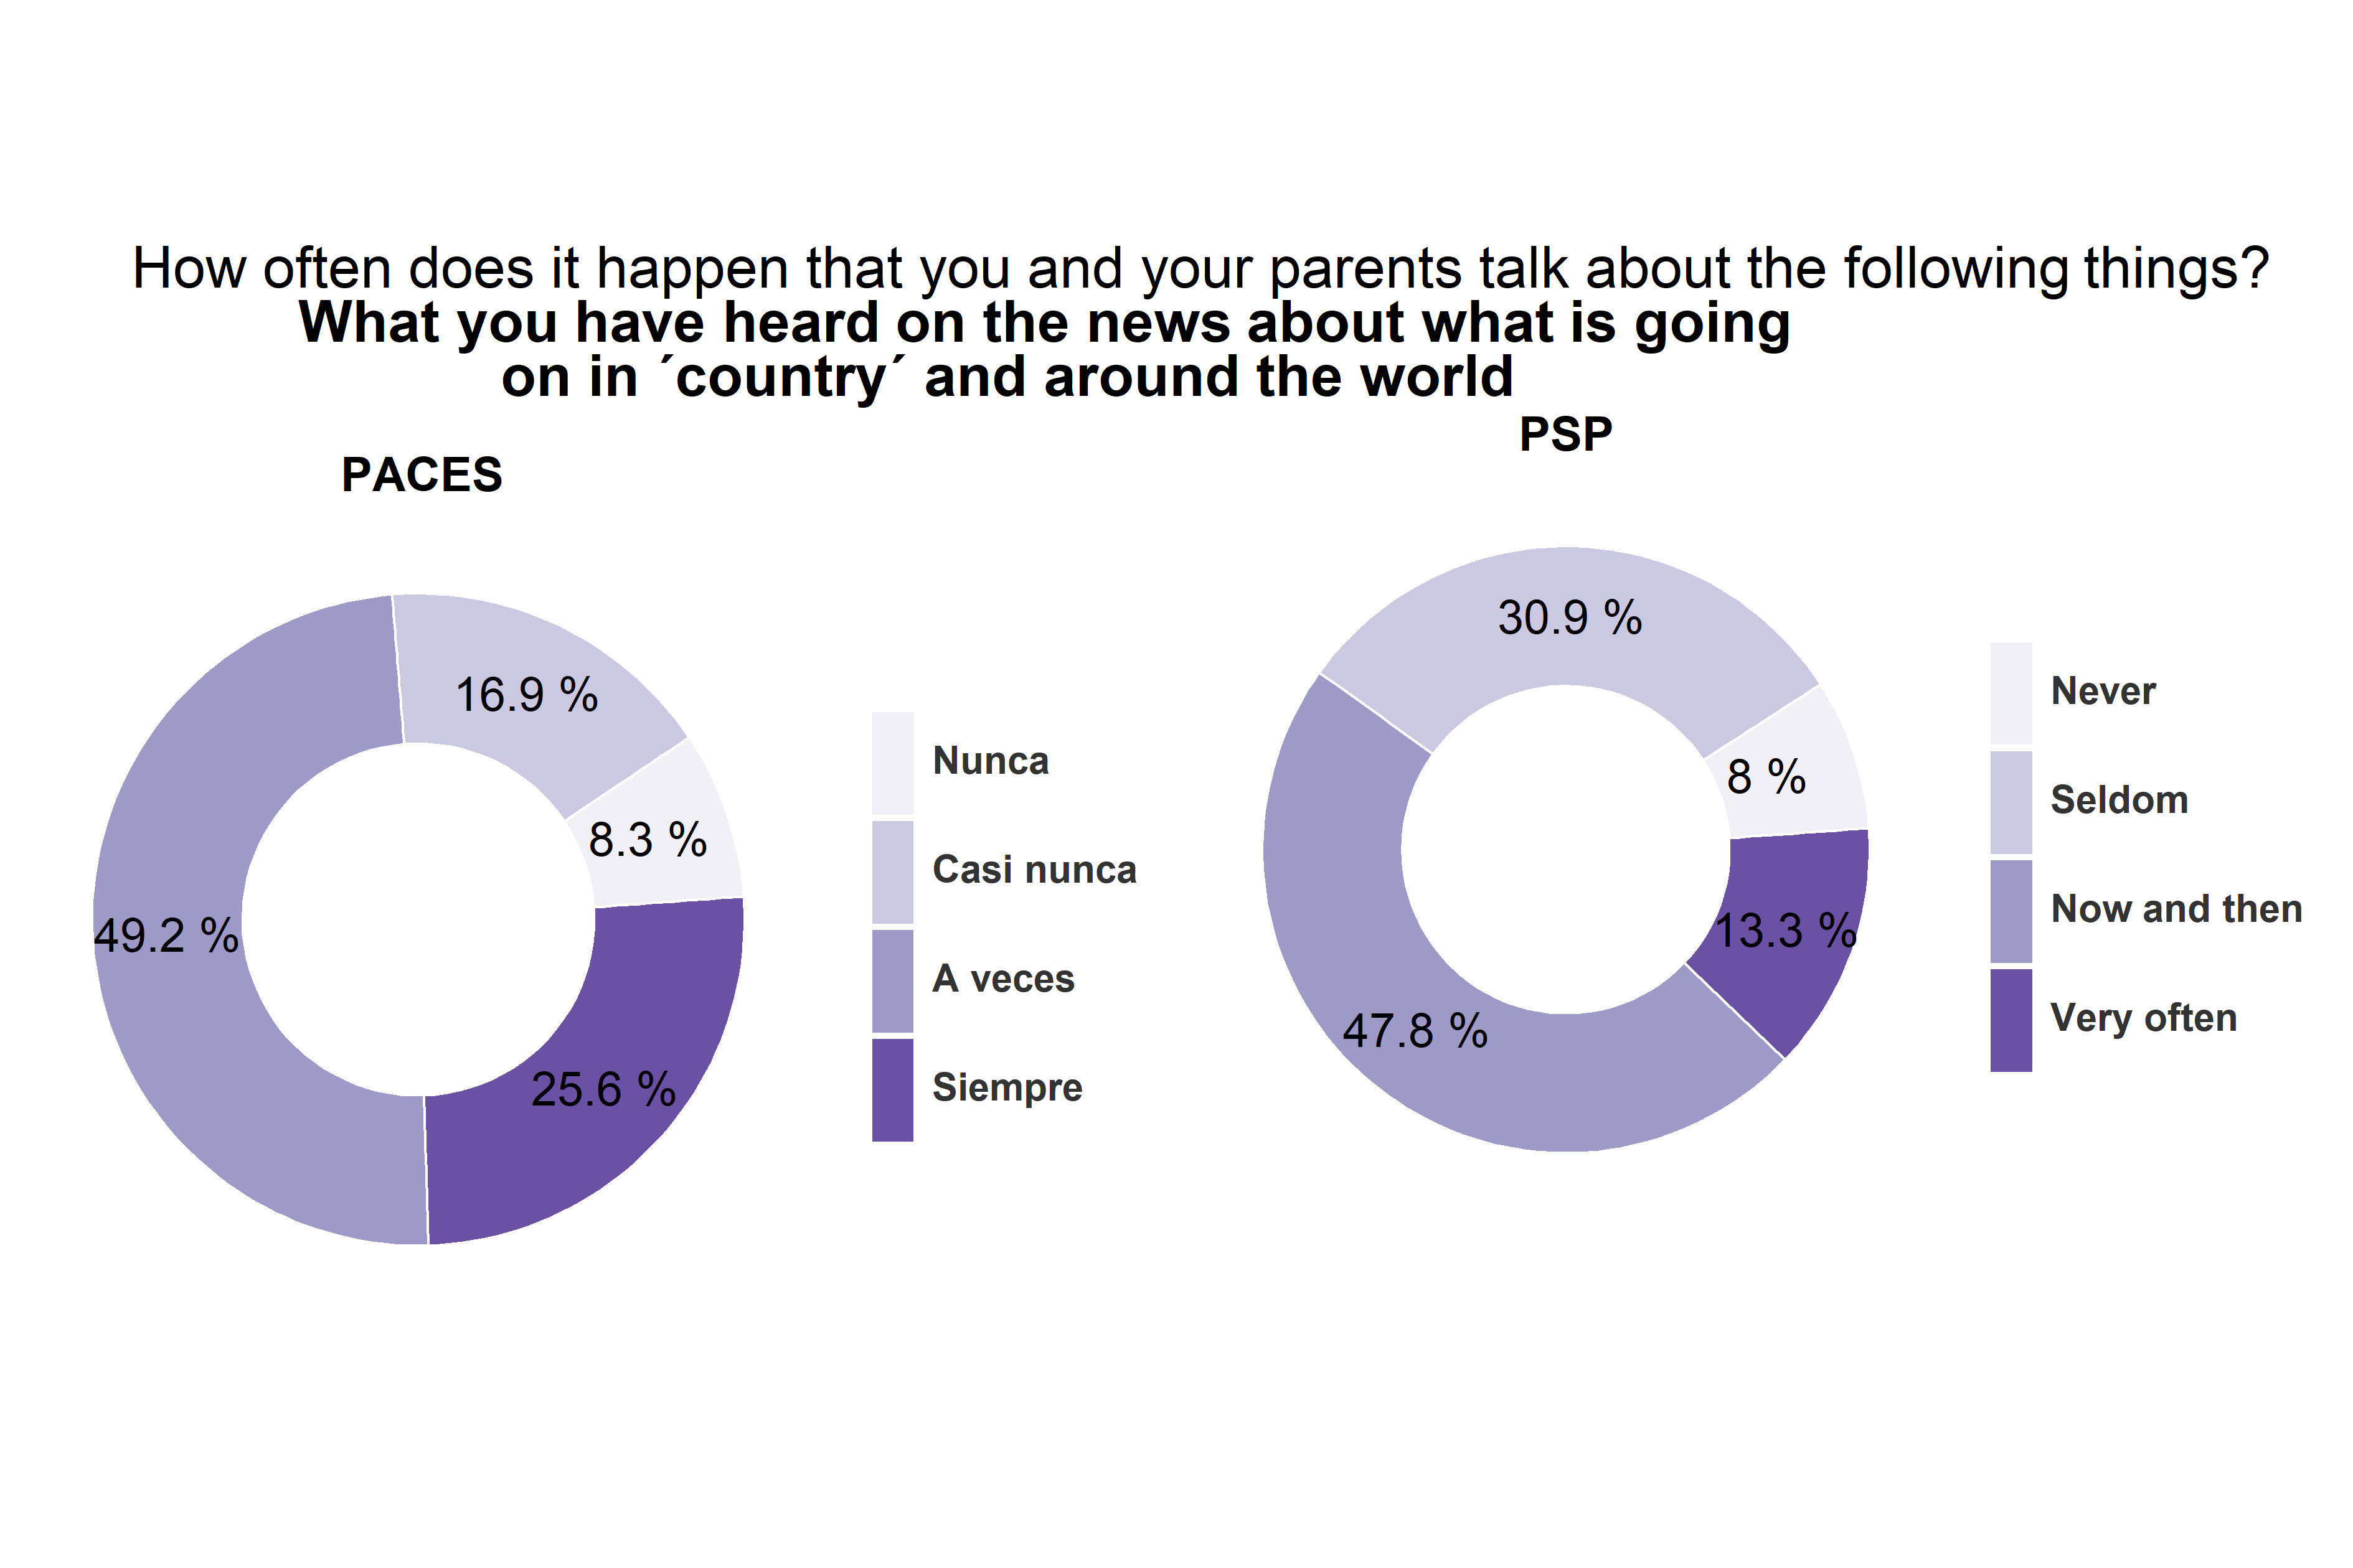
\includegraphics{output/plotdiscpar1.png}

\textbf{Environmental issues}

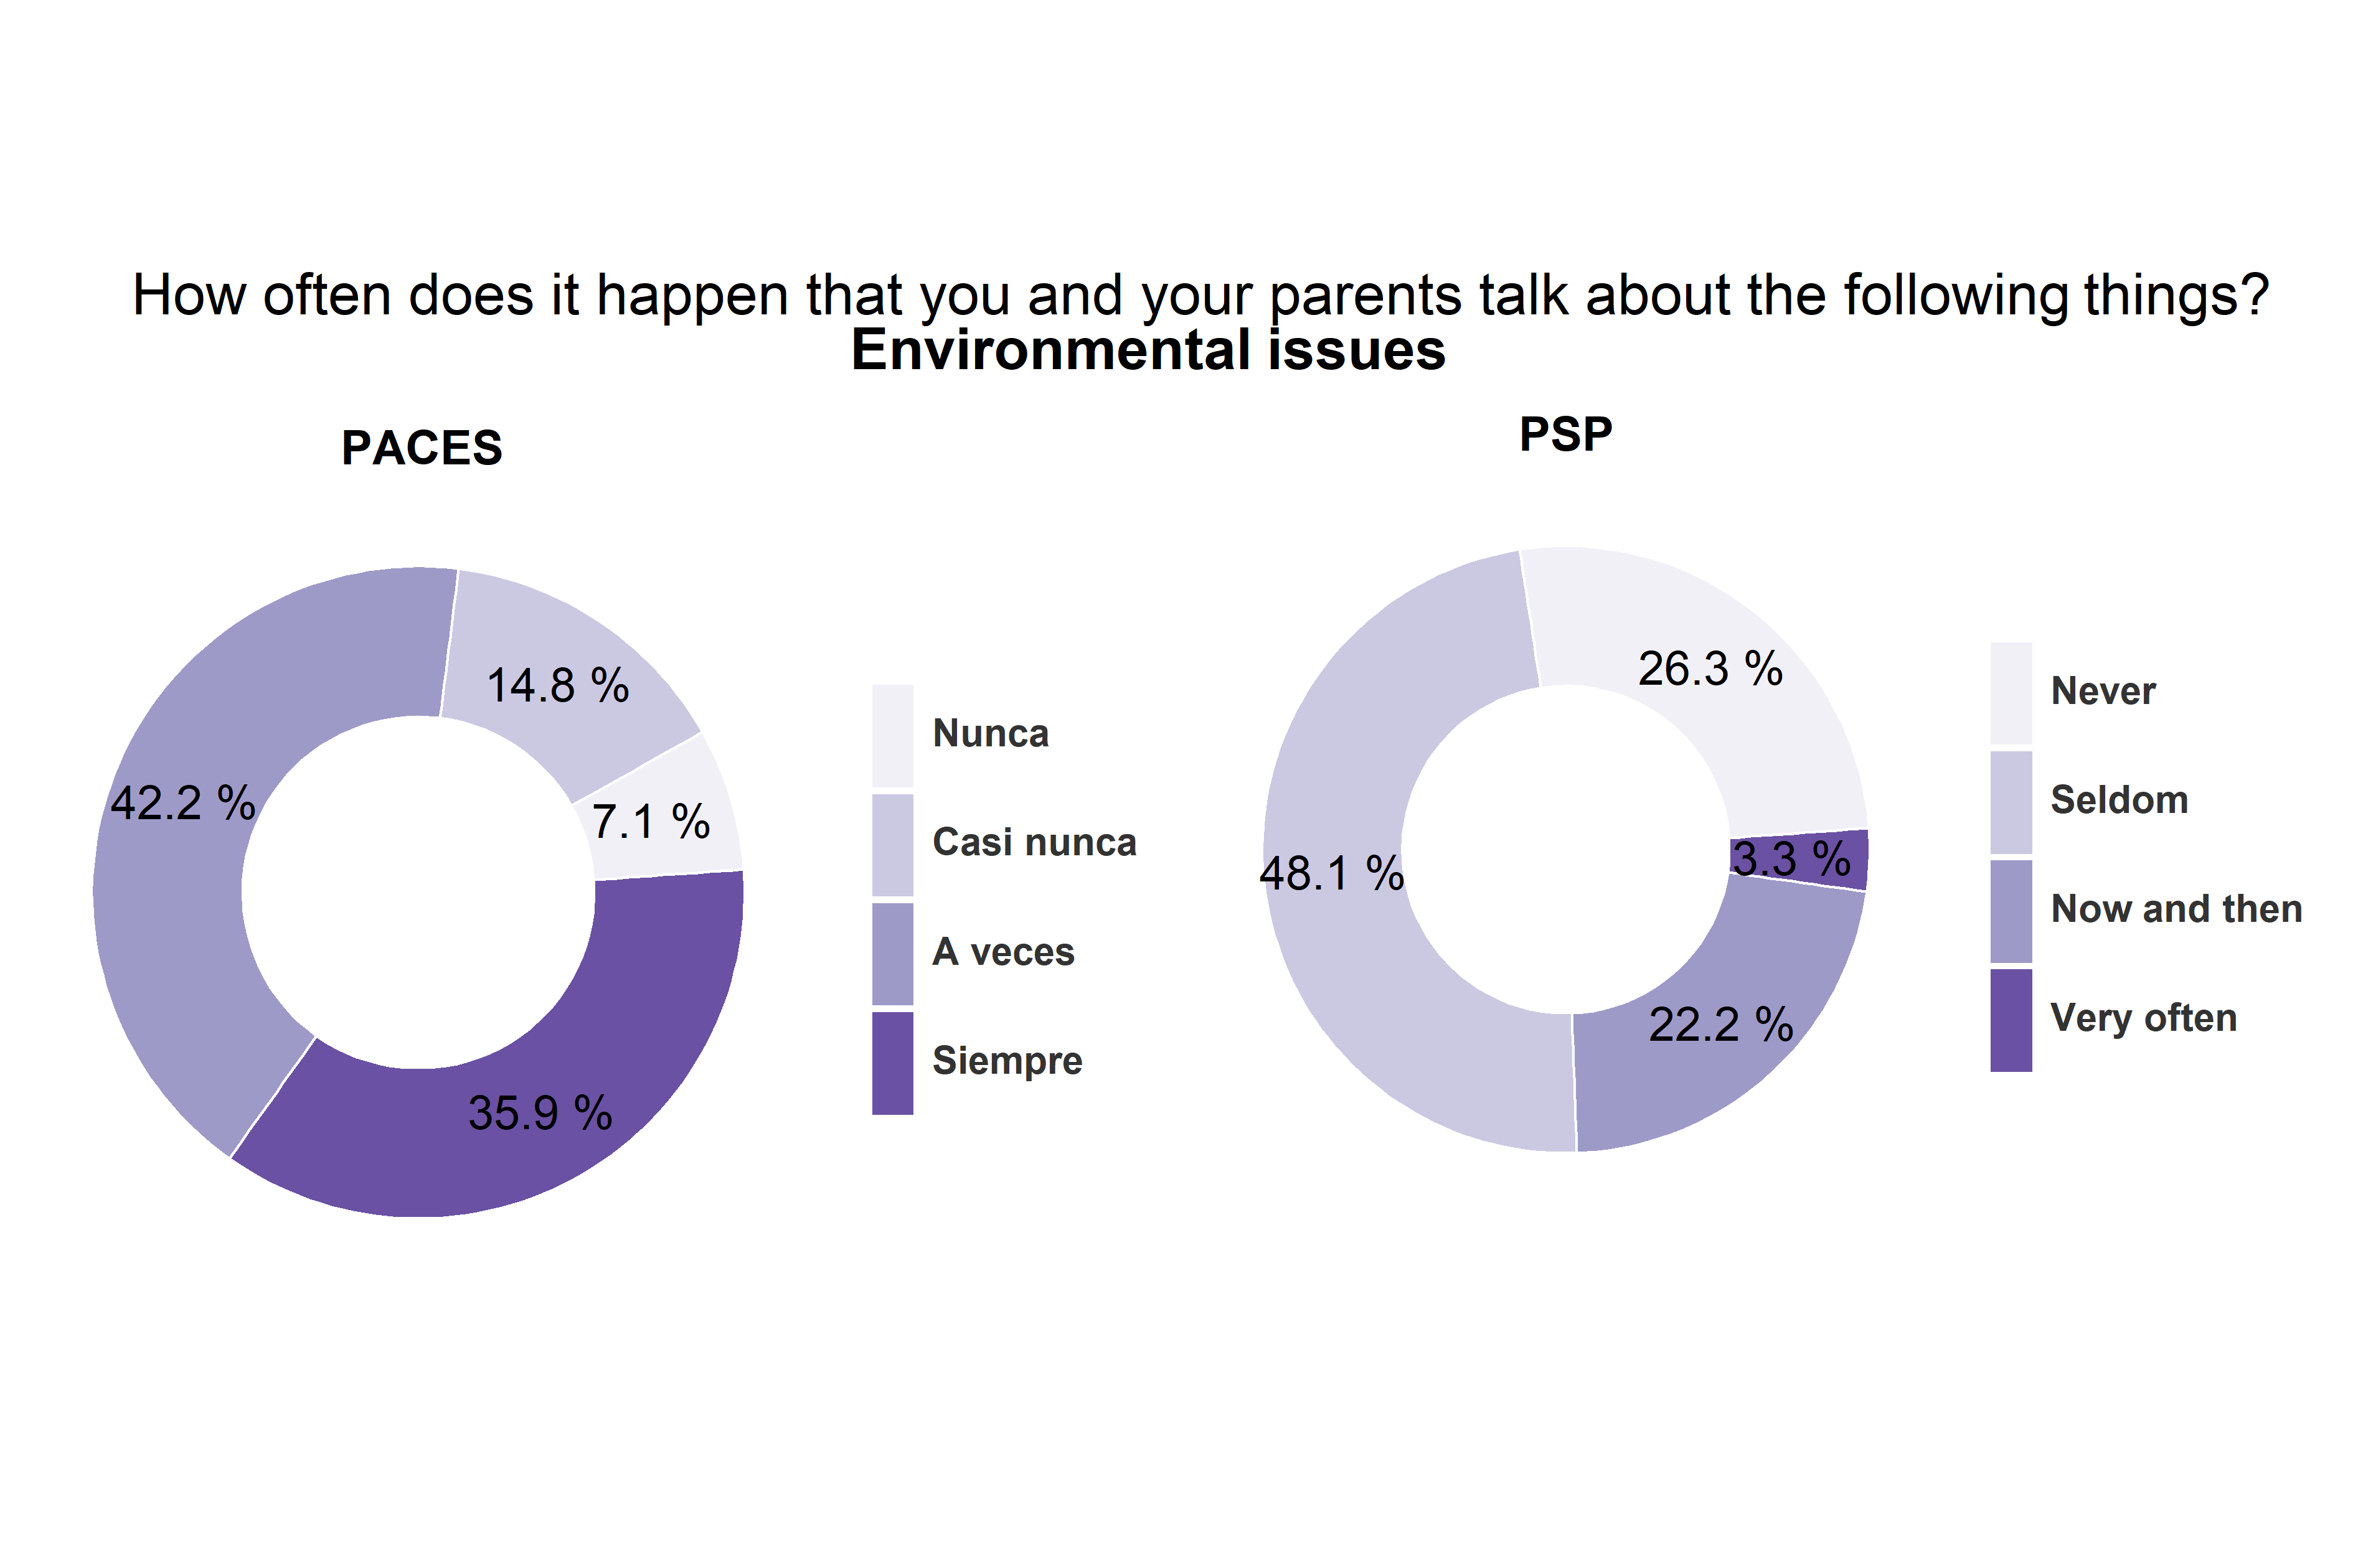
\includegraphics{output/plotdiscpar2.png}

\textbf{Politics or societal issues}

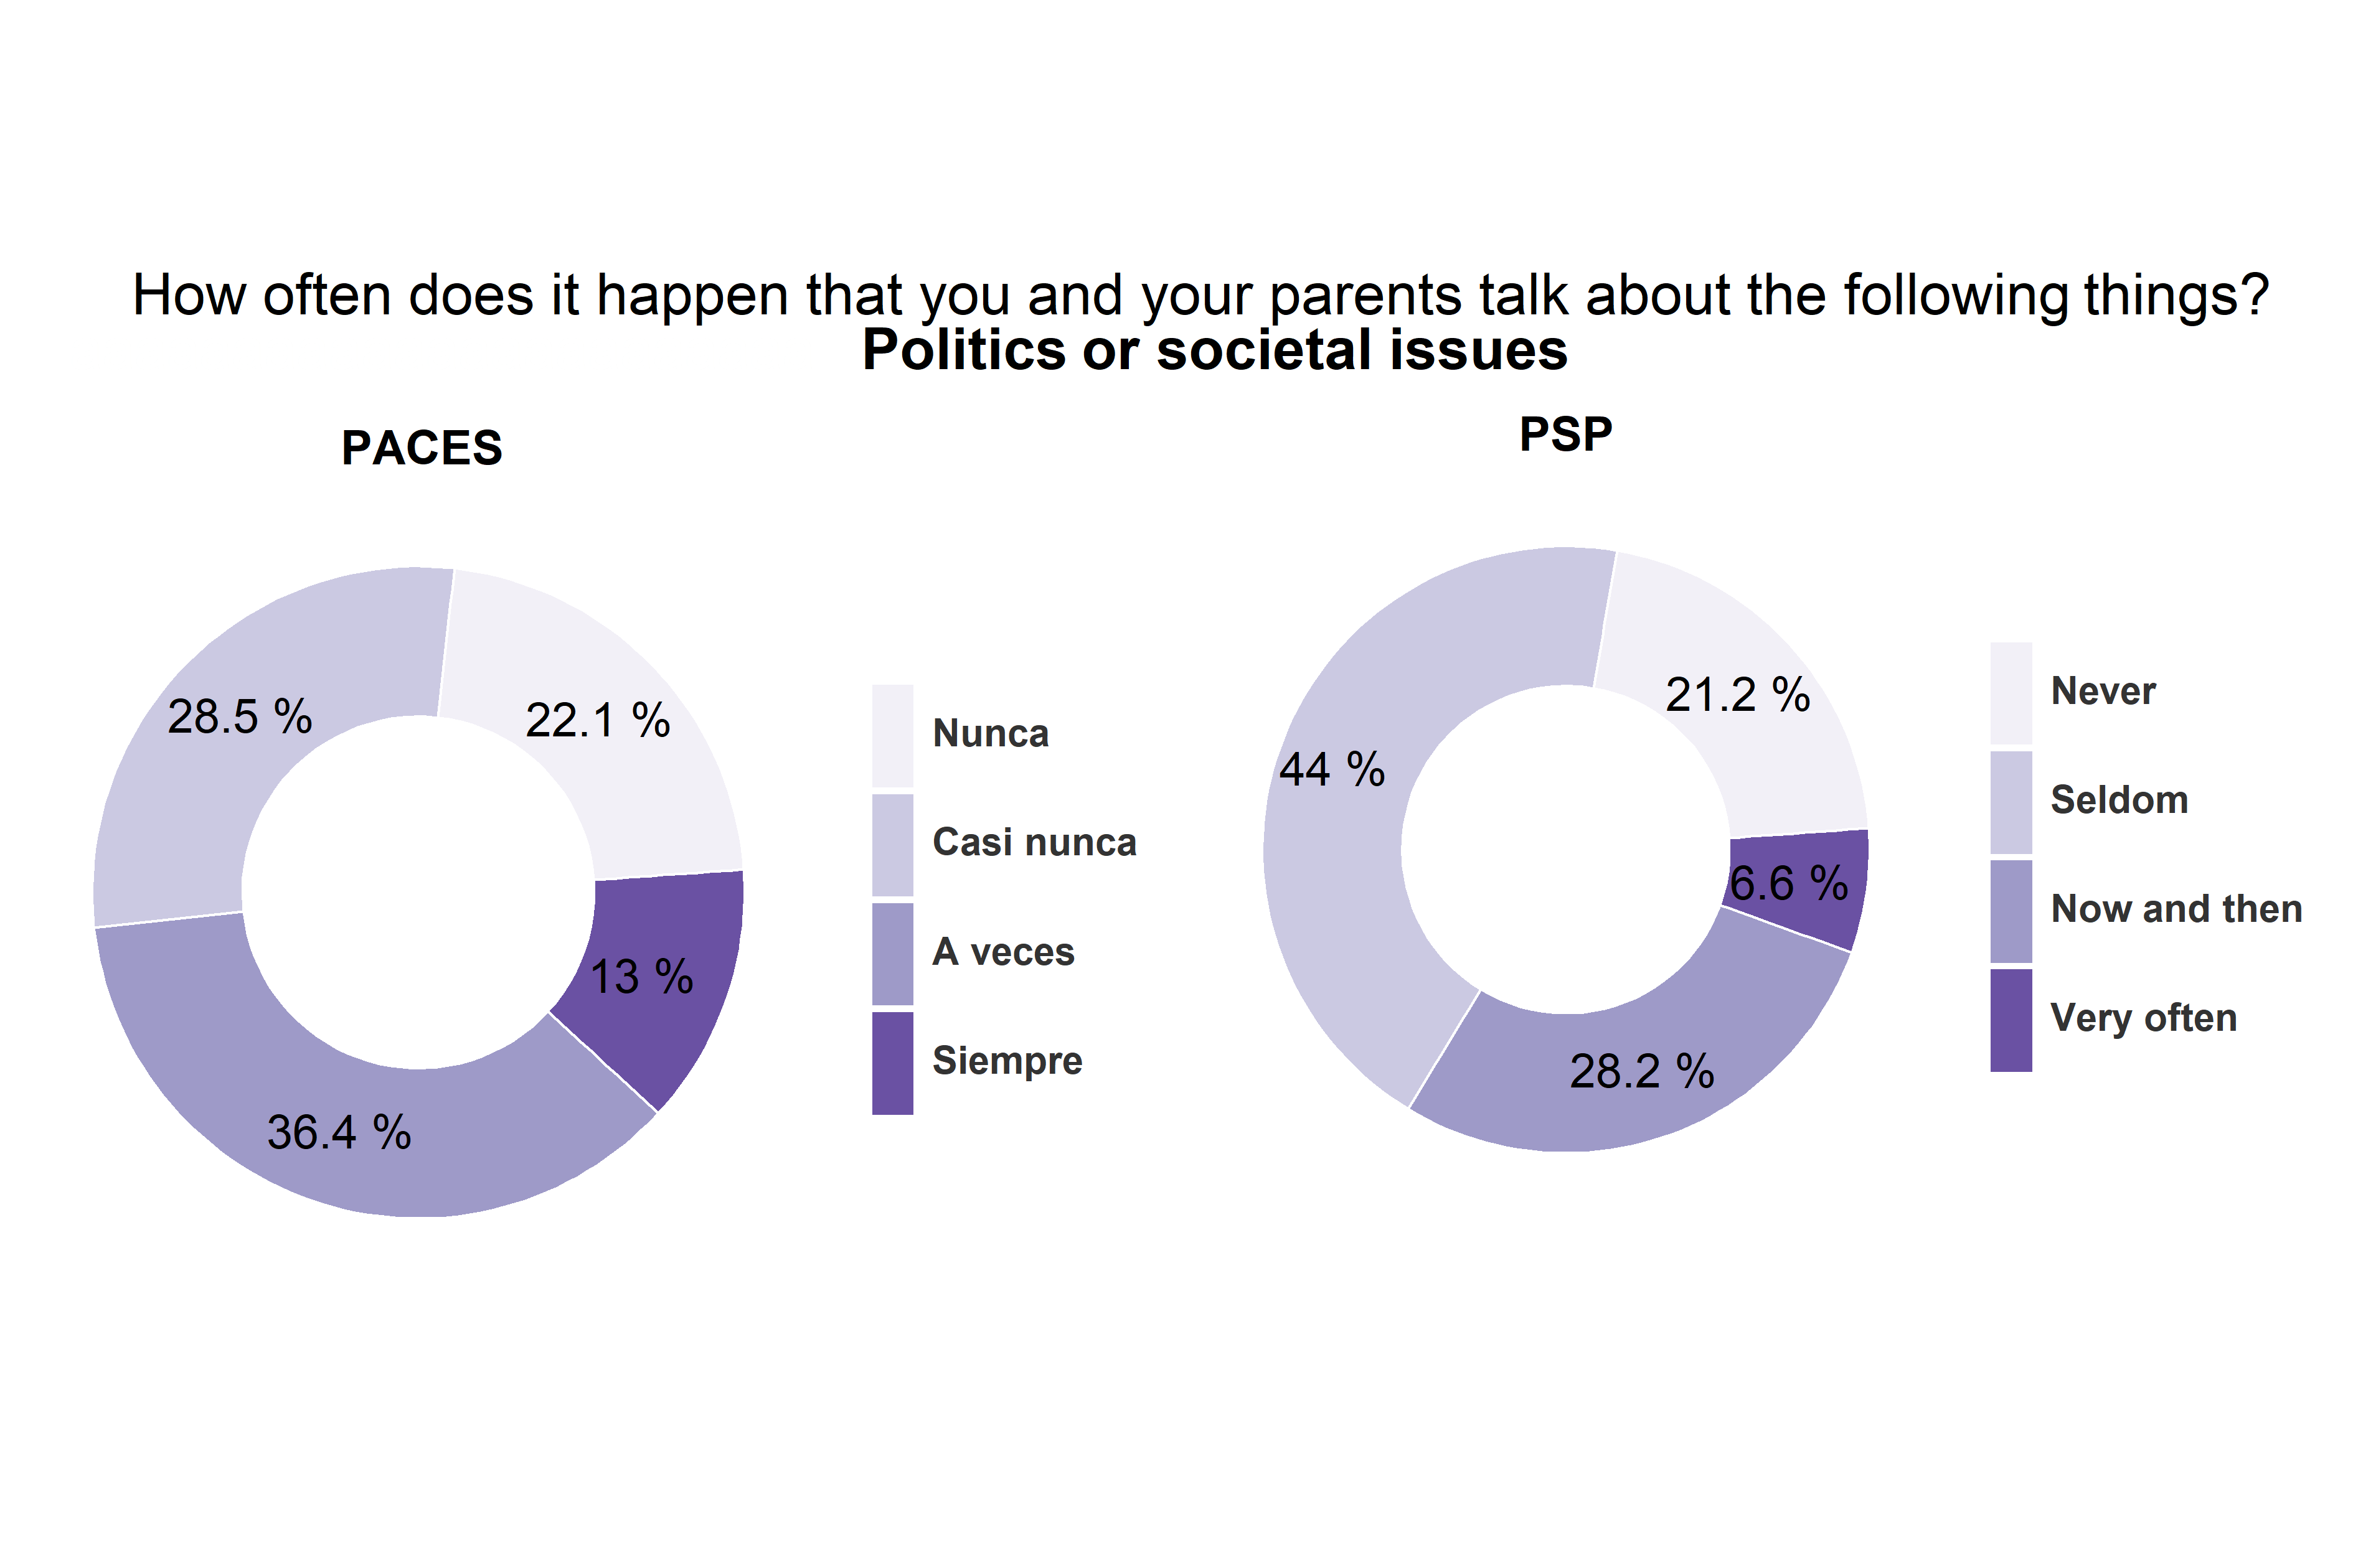
\includegraphics{output/plotdiscpar3.png}

\begin{quote}
ICCS
\end{quote}

\begin{verbatim}
## Error in na.omit(.): objeto 'iccs_chsw' no encontrado
\end{verbatim}

\begin{verbatim}
## Error in na.omit(.): objeto 'iccs_chsw' no encontrado
\end{verbatim}

\begin{verbatim}
## Error in na.omit(.): objeto 'iccs_chsw' no encontrado
\end{verbatim}

\hypertarget{reflexiones-finales}{%
\chapter{Reflexiones finales}\label{reflexiones-finales}}

La comparación entre las democracias Chilena y Sueca nos indica que, aunque ambas son democracias efectivas poseen algunas diferencias de la primera respecto a la segunda. Por un lado, la democracia de Chile se ve afectada por su incapacidad de garantizar algunos derechos propios de los ciudadanos como el acceso a la justicia o algunos derechos sociales. Por otro lado, la democracia Chilena posee una menor estabilidad histórica, siendo esta más bien reciente y estando garantizada solo hace 30 años en este país.

La diferencia de la calidad de la democracia de ambos países posee cierto correlato en la opinión pública de ambos países.

En este contexto institucional y de opinión publica resultan interesantes las diferencias en la vivencia democrática de los jóvenes de ambos países.

Aunque la diferencia de la calidad de la democracia parece expresarse en diferencias en la satisfacción de la misma por parte de los jóvenes de ambos países, no parece tener un correlato con posibles diferencias en los valores democráticos de estos jóvenes ni en su participación. Más bien, se observa que los jóvenes de ambos países poseen una valoración similar de la democracia y de sus valores, a la vez que poseen distintos patrones de participación.

\hypertarget{bibliografuxeda}{%
\chapter*{Bibliografía}\label{bibliografuxeda}}
\addcontentsline{toc}{chapter}{Bibliografía}

% %%%%%%%%%%%%%%%%%%%%%%%%%%%%%%%%%%%%%%%%%%%%%%%%%
% %%% Bibliography                              %%%
% %%%%%%%%%%%%%%%%%%%%%%%%%%%%%%%%%%%%%%%%%%%%%%%%%
% \addtocontents{toc}{\vspace{.5\baselineskip}}
% \cleardoublepage
% \phantomsection
% \addcontentsline{toc}{chapter}{\protect\numberline{}{Bibliography}}
\bibliography{tesis}

%% All books from our library (SfS) are already in a BiBTeX file
%% (Assbib). You can use Assbib combined with your personal BiBTeX file:
%% \bibliography{Myreferences,Assbib}. Of course, this will only work on
%% the computers at SfS, unless you copy the Assbib file
%%  --> /u/sfs/bib/Assbib.bib



\end{document}
